\documentclass{ctexbeamer}
\usepackage{verbatim}
\usepackage{graphicx}
\usepackage{amsmath}
\usepackage{extarrows}
\usepackage{mathtools}
\usepackage{multirow,booktabs}
\usepackage{tikz}
\usepackage{multimedia}
\usepackage{hyperref}
\usepackage{luatex85}
\usepackage{xmpmulti}
%\addtobeamertemplate{block begin}{%
%\setlength{\textwidth}{0.9\textwidth}%
%}{}
\usetikzlibrary{calc,positioning,shapes.misc}
\usetikzlibrary{arrows.meta,graphs,graphdrawing}
\usegdlibrary{layered}
\usepackage{tcolorbox}
\usepackage{empheq}
\usepackage{multirow}
\newcommand*\widefbox[1]{\fbox{\hspace{1em}#1\hspace{1em}}}
%\usetheme{PaloAlto}
%\usetheme{CambridgeUS}
\usetheme[hideallsubsections]{Berkeley}
%\setbeamersize{sidebar width left=0pt}
\logo{
\includegraphics[width=1.55cm,height=1.55cm]{logo.jpg}}
\newcounter{savedenum}
\newcommand*{\saveenum}{\setcounter{savedenum}{\theenumi}}
\newcommand*{\resume}{\setcounter{enumi}{\thesavedenum}}
\AtBeginSection[]{%
\begin{frame}[shrink]
  \frametitle{目录}
  \tableofcontents[currentsection,hideallsubsections]
\end{frame}
}
\AtBeginSubsection[]
{
\begin{frame}[shrink]
  \tableofcontents[sectionstyle=show/shaded,subsectionstyle=show/shaded/hide]
\end{frame}
}


\title[微波技术基础]{《微波技术基础》}
\subtitle{Fundamentals of Microwave Technology}

\author{Yang Jing\inst{1}}
\institute[Sch.EIE HFNU]
{
      \inst{1} %
      School of Electronic Information and Electrical Engineering \\
      Hefei Normal University\\
}

%\includeonly{Chapter5.tex} % 每次编译一章,减少编译量

\begin{document}
\frame{\titlepage}

\begin{frame}{教材}
      《微波技术基础(第2版)》,李秀萍编,电子工业出版社,2017.7.
      \begin{figure}
            \centering
            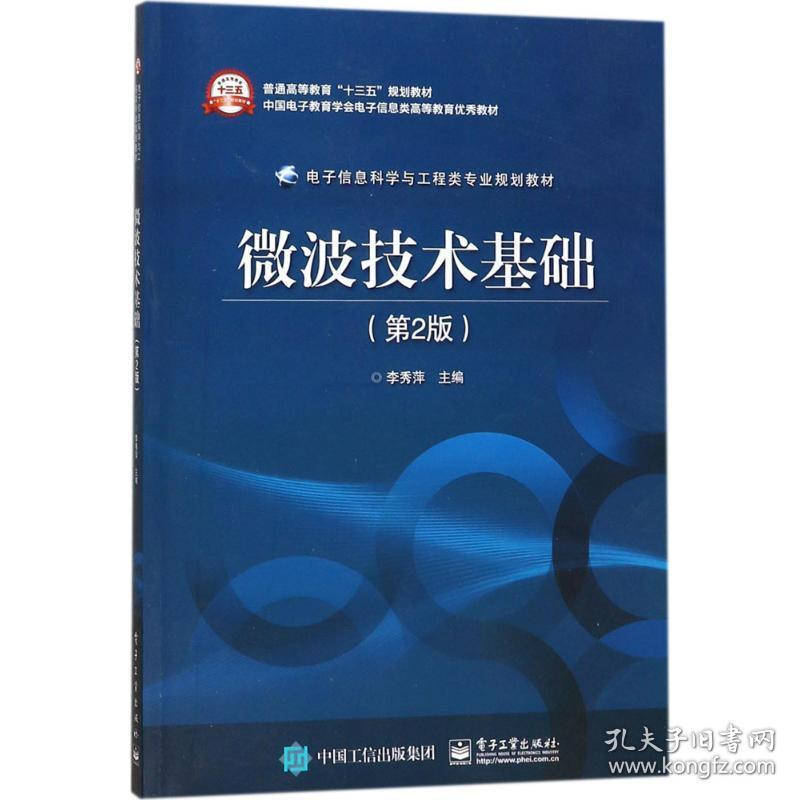
\includegraphics[height=6cm]{jiaocaibeiyou}
      \end{figure}
\end{frame}

\begin{frame}{参考书目}
      \bibliographystyle{apalike}
      \nocite{Zhao}
      \nocite{Wu}
      \nocite{Colin}
      \nocite{Liang}
      \nocite{Liao}
      \bibliography{math}
\end{frame}

\begin{frame}{考核模式}
      \begin{enumerate}
            \item 平时成绩$100$分,占总成绩$50\%$
                  \begin{enumerate}
                        \item 学习态度:$100$分,占$20\%$(考勤 $100$分,占$100\%$)
                        \item 课堂参与:$100$分,占$30\%$(课堂表现,课堂回答问题积极性,$100$分,占$100\%$)
                        \item 平时作业:$100$分,占$50\%$(书面作业$100$分,占$100\%$)
                  \end{enumerate}
            \item 期末考核$100$分,占总成绩$50\%$(期末笔试$100$分,占$100\%$)
      \end{enumerate}
\end{frame}

\documentclass{ctexbeamer}
\usepackage{verbatim}
\usepackage{graphicx}
\usepackage{amsmath}
\usepackage{mathtools}
\usepackage{multirow,booktabs}
\usepackage{tikz}
%\addtobeamertemplate{block begin}{%
%\setlength{\textwidth}{0.9\textwidth}%
%}{}
\usetikzlibrary{positioning}
\usetikzlibrary{calc}
\usepackage{tcolorbox}
\usepackage{empheq}
\newcommand*\widefbox[1]{\fbox{\hspace{1em}#1\hspace{1em}}}
%\usetheme{PaloAlto}
%\usetheme{CambridgeUS}
\usetheme{Berkeley}
\logo{
\includegraphics[width=1.55cm,height=1.55cm]{logo.jpg}}
\newcounter{savedenum}
\newcommand*{\saveenum}{\setcounter{savedenum}{\theenumi}}
\newcommand*{\resume}{\setcounter{enumi}{\thesavedenum}}

\begin{document}
\begin{frame}
  \title{《微波技术基础》}
  \institute{Sch.EIEE Hefei Normal University}
  \author{杨晶}
  \date{\today}
  \titlepage
\end{frame}

\begin{frame}{目录}
  \tableofcontents
\end{frame}

\begin{frame}{教材}
  《微波技术基础》,廖承恩编,西安电子科技大学出版社,2011.5.
  \begin{figure}
    \centering
    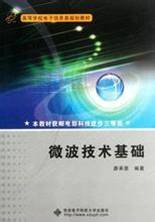
\includegraphics[height=6cm]{jiaocai}
  \end{figure}
\end{frame}

\begin{frame}{参考文献}
  \bibliographystyle{apalike}
  \nocite{Zhao}
  \nocite{Wu}
  \nocite{Colin}
  \nocite{Liang}
  \bibliography{math}
\end{frame}

\begin{frame}{考核模式}
  \begin{enumerate}
    \item 平时成绩$100$分,占总成绩$50\%$
    \begin{enumerate}
    \item 学习态度:$100$分,占$20\%$(考勤 $100$分,占$100\%$)
    \item 课堂参与:$100$分,占$30\%$(课堂表现,课堂回答问题积极性,$100$分,占$100\%$)
    \item 平时作业:$100$分,占$50\%$(书面作业$100$分,占$100\%$)
    \end{enumerate}
    \item 期末考核$100$分,占总成绩$50\%$(期末笔试$100$分,占$100\%$)
  \end{enumerate}
\end{frame}

\begin{frame}{微波技术基础}
  \begin{description}
    \item[第一章] \textcolor{red}{引论}
    \item[第二章] \textcolor{red}{传输线理论}
    \item[第三章] \textcolor{red}{规则金属波导}
    \item[第四章] \textcolor{red}{微波集成传输线}
    \item[第五章] 毫米波介质波导与光波导
    \item[第六章] \textcolor{red}{微波网络基础}
    \item[第七章] \textcolor{red}{微波谐振器}
    \item[第八章] \textcolor{red}{常用微波元件}
    \item[第九章] 微波铁氧体元件
  \end{description}
\end{frame}

\section{第一章\quad 引论}
\begin{frame}{第一章\quad 引论}
  \begin{enumerate}
    \item 微波及其特点
    \item 微波的应用
    \item 本书的内容框图
    \item 导行波及其一般的传输特性
  \end{enumerate}
\end{frame}

\begin{frame}{近代通信技术的发展}
  \begin{columns}
    \begin{column}{0.35\linewidth}
      \centering
      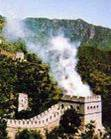
\includegraphics[height=5cm]{fenghuotai}
    \end{column}
    \begin{column}{0.65\linewidth}
      \centering
      \begin{itemize}
        \item 人类历史上最早的通信手段和现在一样是“无线”的。
        \item 人类通信史上革命性变化,是从把电作为信息载体后发生的。
      \end{itemize}
    \end{column}
  \end{columns}
\end{frame}

\begin{frame}{电报的发明}
  \begin{columns}
    \begin{column}{0.5\linewidth}
      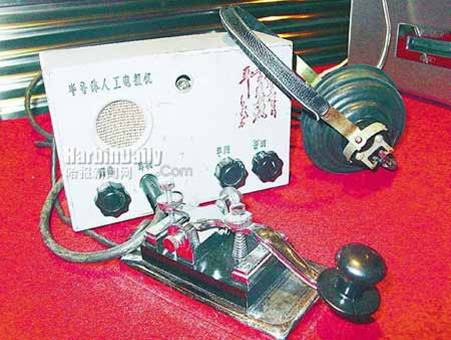
\includegraphics[height=4cm]{dianbao}
    \end{column}
    \begin{column}{0.5\linewidth}
      \begin{itemize}
        \item 电报的发明,拉开了电信时代的序幕,开创了人类利用电来传递信息的历史。
      \end{itemize}
    \end{column}
  \end{columns}
\end{frame}

\begin{frame}{电报的发明}
  \begin{columns}
    \begin{column}{0.5\linewidth}
    \begin{figure}
      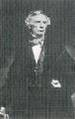
\includegraphics[width=3.5cm]{Morse.jpg}
      \caption{莫尔斯 Morse.Samrel Finley.Breese (1791-1872)}\label{Morse}
    \end{figure}
    \end{column}
    \begin{column}{0.5\linewidth}
      \begin{itemize}
        \item 美国画家莫尔斯
        \item 在1835年,第一台电报机问世
      \end{itemize}
    \end{column}
  \end{columns}
\end{frame}

\begin{frame}{电报的发明}
  \begin{itemize}
    \item 莫尔斯成功地利用电流的“通”、“断”和“长断”来代替了人类的文字进行传送,这就是鼎鼎大名的莫尔斯电码。
  \end{itemize}
  \centering
  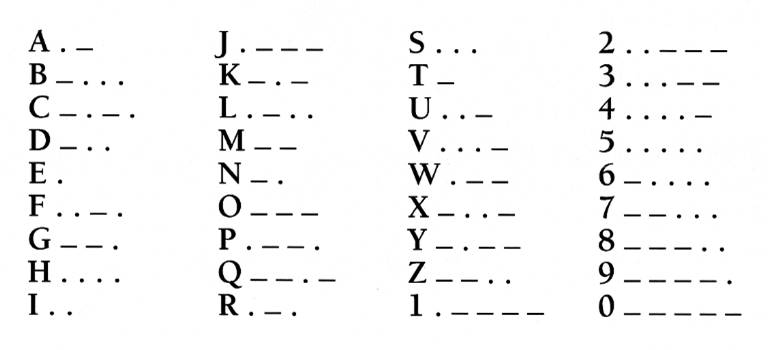
\includegraphics[width=8cm]{morsecode}
\end{frame}

\begin{frame}{电话的发明}
  \begin{columns}
    \begin{column}{0.35\linewidth}
      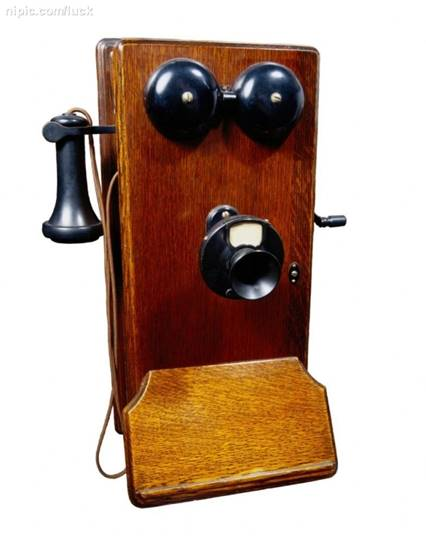
\includegraphics[height=6.5cm]{dianhua}
    \end{column}
    \begin{column}{0.65\linewidth}
      \begin{itemize}
        \item 1875年6月2日,被人们作为发明电话的伟大日子而加以纪念,而美国波士顿法院路109号也因此载入史册,至今它的门口仍钉着块铜牌,上面镌有:“1875年6月2日电话诞生在此。”
      \end{itemize}
    \end{column}
  \end{columns}
\end{frame}

\begin{frame}{电话的发明}
  \begin{columns}
    \begin{column}{0.4\linewidth}
    \begin{figure}
      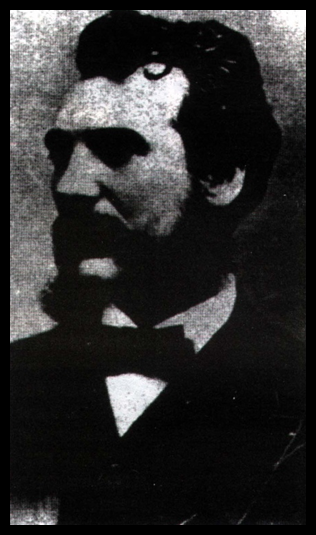
\includegraphics[width=3.2cm]{Bell.png}
      \caption{亚历山大·格拉汉姆·贝尔Alexander Graham Bell (1847 - 1922)}
    \end{figure}
    \end{column}
    \begin{column}{0.6\linewidth}
      \begin{itemize}
        \item 美国发明家和企业家。他获得了世界上第一台可用的电话机的专利权(发明者为意大利人安东尼奥·梅乌奇),创建了贝尔电话公司(AT\&T公司的前身)。其被世界誉为“电话之父”。
      \end{itemize}
    \end{column}
  \end{columns}
\end{frame}

\begin{frame}{电话的发明}
  \begin{columns}
    \begin{column}{0.5\linewidth}
      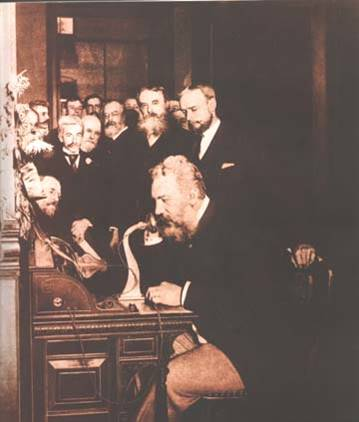
\includegraphics[width=5.5cm]{Bell2}
    \end{column}
    \begin{column}{0.5\linewidth}
      \begin{itemize}
        \item 贝尔在1892年启用第一条长途电话线——从纽约至芝加哥,长约900里。
      \end{itemize}
    \end{column}
  \end{columns}
\end{frame}

\begin{frame}{电话的发明}
  \begin{columns}
    \begin{column}{0.35\linewidth}
      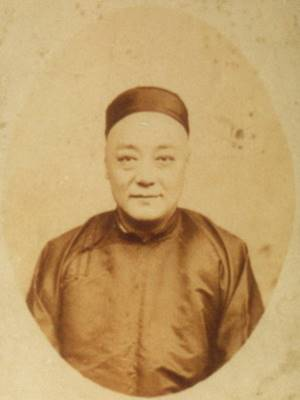
\includegraphics[width=3.5cm]{pengmingbao}
    \end{column}
    \begin{column}{0.65\linewidth}
      \begin{itemize}
        \item 电话传入我国,是在1881年,英籍电气技师皮晓浦在上海十六铺沿街架起一对露天电话,付36文制钱可通话一次,这是中国的第一部电话。1882年2月,丹麦大北电报公司在上海外滩扬于天路办起我国第一个电话局,用户25家。
        \item 1889年,安徽省安庆州候补知州\textbf{彭名保},自行设计了一部电话,包括自制的五六十种大小零件,称为我国第一部自行设计制造的电话。
      \end{itemize}
    \end{column}
  \end{columns}
\end{frame}

\begin{frame}{电磁波的发现}
  % Electromagnetic wave - black
\begin{tikzpicture}[x=(-15:0.9), y=(90:1.0), z=(-150:1.0),
                    line cap=round, line join=round,
                    axis/.style={black, thick,->},
                    vector/.style={>=stealth,->}]
  \large
  \def\A{1}
  \def\nNodes{5} % use even number
  \def\nVectorsPerNode{8}
  \def\N{\nNodes*40}
  \def\xmax{\nNodes*pi/2*1.01}
  \pgfmathsetmacro\nVectors{(\nVectorsPerNode+1)*\nNodes}

  \def\vE{{\color{blue}\mathbf{E}}}
  \def\vB{{\color{red}\mathbf{B}}}
  \def\vk{\mathbf{\hat{k}}}

  % main axes
  \draw[axis] (0,0,0) -- ++(\xmax*1.1,0,0) node[right] {$x$};
  \draw[axis] (0,-\A*1.4,0) -- (0,\A*1.4,0) node[right] {$y$};
  \draw[axis] (0,0,-\A*1.4) -- (0,0,\A*1.4) node[above left] {$z$};

  % small axes
  \def\xOffset{{(\nNodes-2)*pi/2}}
  \def\yOffset{\A*1.2}
  \def\zOffset{\A*1.2}
  \draw[axis] (\xOffset,\yOffset,-\zOffset) -- ++(\A*0.6,0,0) node[right] {$\vk$};
  \draw[axis] (\xOffset,\yOffset,-\zOffset) -- ++(0,\A*0.6,0) node[right] {$\vE$};
  \draw[axis] (\xOffset,\yOffset,-\zOffset) -- ++(0,0,\A*0.6) node[above left] {$\vB$};

  % equation
  %\node[above right] at (\xOffset,-0.5*\yOffset,4*\zOffset)
  %  {$\begin{aligned}
  %    \vE &= \mathbf{E_0}\sin(\vk\cdot\mathbf{x}-c_0t)\\
  %    \vB &= \mathbf{B_0}\sin(\vk\cdot\mathbf{x}-c_0t)\\
  %    \end{aligned}$};
  %\node[below right] at (\xOffset,-0.5*\yOffset,4*\zOffset)
  %  {$\vE\cdot\vk = 0,\;\; \vB\cdot\vk = 0,\;\; \vB = \frac{1}{c_0}\vk\times\vE$};

  % waves
  \draw[blue,very thick,variable=\t,domain=0:\nNodes*pi/2*1.01,samples=\N]
    plot (\t,{\A*sin(\t*360/pi)},0);
  \draw[red,very thick,variable=\t,domain=0:\nNodes*pi/2*1.01,samples=\N]
    plot (\t,0,{\A*sin(\t*360/pi)});

  % draw vectors
  \foreach \k [evaluate={\t=\k*pi/2/(\nVectorsPerNode+1);
                         \angle=\k*90/(\nVectorsPerNode+1);
                         \c=(mod(\angle,90)!=0);}]
              in {1,...,\nVectors}{
    \if\c1
      \draw[vector,blue!50] (\t,0,0) -- ++(0,{\A*sin(2*\angle)},0);
      \draw[vector,red!50] (\t,0,0) -- ++(0,0,{\A*sin(2*\angle)});
    \fi
  }
\end{tikzpicture}
\begin{itemize}
  \item 自从贝尔发明了电话机,这样人人都能手拿一个“话柄”,和远方的亲朋好友谈天说地了。电报和电话的相继发明,使人类获得了远距离传送信息的重要手段。但是,电信号都是通过金属线传送信息的重要手段。但是,电信号都是通过金属线传送的。线路架设到的地方,信息才能传到,这就大大限制了信息的传播范围,特别是在大海、高山,有没有能让信息\textbf{无线}传播的方法?
\end{itemize}
\end{frame}

\begin{frame}{电磁波的发现}
  \begin{columns}
    \begin{column}{0.35\linewidth}
    \begin{figure}
      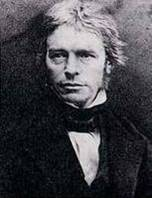
\includegraphics[width=3.5cm]{faraday.jpg}
      \caption{迈克尔·法拉第Michael Faraday(1791-1867)}
    \end{figure}
    \end{column}
    \hfill
    \begin{column}{0.65\linewidth}
      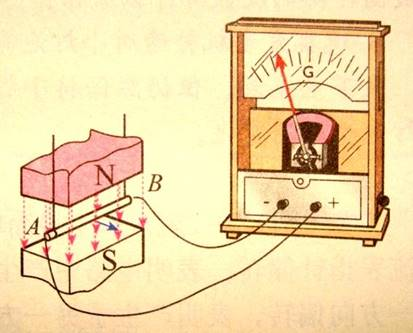
\includegraphics[width=5cm]{faradayexperiment.jpg}
      \begin{itemize}
        \item 英国物理学家、化学家
        \item 1831年发现电磁感应
      \end{itemize}
    \end{column}
  \end{columns}
\end{frame}

\begin{frame}{电磁波的发现}
  \begin{columns}
    \begin{column}{0.35\linewidth}
      \begin{figure}
        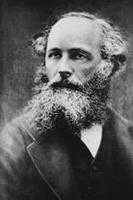
\includegraphics[width=3.5cm]{maxwell.jpg}
        \caption{詹姆斯·克拉克·麦克斯韦James Clerk Maxwell (1831-1879)}
      \end{figure}
    \end{column}
    \begin{column}{0.65\linewidth}
      Maxwell Equations:
      %\begin{equation}
        \begin{align*}
          &\nabla\times\vec E=-\frac{\partial \vec B}{\partial t}\\
          &\nabla\times\vec H=\vec{J} +\frac{\partial \vec D}{\partial t}\\
          &\nabla\cdot\vec{D}=\rho\\
          &\nabla\cdot\vec{B}=0
        \end{align*}
      %\end{equation}
      \begin{itemize}
        \item 英国物理学家。1864年,麦氏发表了电磁场理论,成为人类历史上预言电磁波存在的\textbf{第一人}
      \end{itemize}
    \end{column}
  \end{columns}
\end{frame}

\begin{frame}{电磁波的发现}
  \begin{columns}
    \begin{column}{0.35\linewidth}
      \begin{figure}
        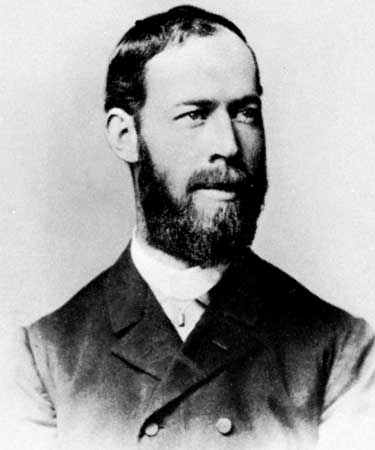
\includegraphics[width=3cm]{hertz.jpg}
        \caption{亨利希·鲁道夫·赫兹(1857 - 1894)}
      \end{figure}
    \end{column}
    \begin{column}{0.65\linewidth}
      \begin{figure}
        \flushright
        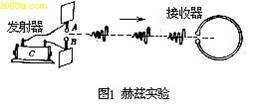
\includegraphics[width=2.5cm]{hertzexperiment.jpg}
      \end{figure}
      \begin{itemize}
        \item 德国物理学家,1887年,实验证实了电磁波的存在和传播。成为了近代科学技术史的一座里程碑,为了纪念这位杰出的科学家,电磁波的单位便命名为“赫兹($Hz$)”
        \item 证明了麦克斯韦理论的正确,导致了无线电的诞生,开辟了电子技术的新纪元,标志着从“有线电通信”向“无线电通信”的转折点。也是整个移动通信的发源点,应该说,从这时开始,人类开始进入了无线通信的新领域。
      \end{itemize}
    \end{column}
  \end{columns}
\end{frame}

\subsection{1\quad 微波及其特点}
\begin{frame}{微波及其特点}
  电磁波按波长(或频率)划分,则大致可以把$300MHz - 3000GHz$,(对应空气中波长$\lambda$是$1m - 0.1mm$)这一频段的电磁波称之为微波。它处于超短波和红外光波之间。
\end{frame}

\begin{frame}{微波波段的划分}
  \begin{tabular}{cccc}
    \toprule
    波段代号 & 标称波长/cm & 频率范围/GHz & 波长范围/cm \\
    \midrule
     L & 22 & 1-2 & 30-15 \\
     S & 10 & 2-4 & 15-7.5 \\
     C & 5 & 4-8 & 7.5-3.5 \\
     X & 3 & 8-12 & 3.75-2.5 \\
     Ku & 2 & 12-18 & 2.5-1.67 \\
     K & 1.25 & 18-27 & 1.67-1.11 \\
     Ka & 0.8 & 27-40 & 1.11-0.75 \\
     U & 0.6 & 40-60 & 0.75-0.5 \\
     V & 0.4 & 60-80 & 0.5-0.375 \\
     W & 0.3 & 80-100 & 0.375-0.3 \\
     \bottomrule
  \end{tabular}
\end{frame}

\begin{frame}{Maxwell方程组的物理意义}
  \begin{columns}
    \begin{column}{0.4\linewidth}
      \begin{align*}
        & \nabla\times\vec{E} = -\frac{\partial \vec{B}}{\partial t}\\
        & \nabla\times\vec{H} = \vec{J}+\frac{\partial \vec{D}}{\partial t}
      \end{align*}
    \end{column}
    \begin{column}{0.6\linewidth}
      \begin{itemize}
        \item 这两个方程左边物理量为磁(或电),而右边物理量则为电(或磁)。这中间的等号深刻揭示了电与磁的相互转化,相互依赖,相互对立,共存于统一的电磁波中。正是由于电不断转换为磁,而磁又不断转换成为电,才会发生能量交换和贮存。
      \end{itemize}
    \end{column}
  \end{columns}
\end{frame}

\begin{frame}{电与磁的转换}
  \begin{itemize}
    \item Oersted和Faraday的实验证实了电磁转换,而且还知道了只有动磁才能转化为电。
    \item 还需提到:电磁转换为电磁波的出现提供了可能,但不一定是现实。例如电磁振荡也是典型的电磁转换,但没有引起\textbf{波(Wave)}。
    \item 作为力学类比,电磁转换犹如单摆问题中的动能与势能的转化。
  \end{itemize}
\end{frame}

\begin{frame}{Maxwell方程组的物理意义}
  \begin{itemize}
    \item 进一步研究Maxwell方程两边的运算,从物理上看,运算反映一种作用(Action)。方程左边是空间运算(\textbf{旋度});方程右边是时间运算(\textbf{导数}),中间用等号连接。它深刻揭示了电(或磁)场任一地点的变化会转化为磁(或电)场时间的变化;反过来,场的时间变化也会转化成地点的变化。正是这种空间和时间的相互变化构成了波动的外在形式。用通俗的一句话说:即\textbf{一个地点出现过的事物,过了一段时间又在另一地点出现了}。
  \end{itemize}
\end{frame}

\begin{frame}{Maxwell方程组的物理意义}
  \begin{columns}
    \begin{column}{0.4\linewidth}
      \begin{align*}
        & \nabla\times\vec{H} = j\omega\epsilon\vec{E}+\vec{J}\\
        & \nabla\times\vec{E} = -j\omega\mu\vec{H}
      \end{align*}
    \end{column}
    \begin{column}{0.6\linewidth}
      \textbf{单色波}频域的$Maxwell$方程
    \end{column}
  \end{columns}
\begin{itemize}
  \item $Maxwell$方程还指出:电磁转化有一个重要条件,即频率$\omega$。只有较高的$\omega$才能确保电磁的有效转换,直流情况没有转换。可以这样说,在高频封闭电路才有可能变成开放电路。不过很有意思的是频率越高,越难输出功率,这也是一个有趣的矛盾。
\end{itemize}
\end{frame}

\begin{frame}{Maxwell方程组的物理意义}
  \begin{columns}
    \begin{column}{0.4\linewidth}
      \begin{align*}
        &\nabla\times\vec E=-\frac{\partial \vec B}{\partial t}\\
        &\nabla\times\vec H=\vec{J} +\frac{\partial \vec D}{\partial t}\\
        &\nabla\cdot\vec{D}=\rho\\
        &\nabla\cdot\vec{B}=0
      \end{align*}
    \end{column}
    \begin{column}{0.65\linewidth}
      \begin{itemize}
        \item 在Maxwell方程中还存在另一对矛盾对抗,这就构成了Maxwell方程本质的不对称性。尽管为了找其对称性而一直在探索磁流$\vec{M}$的存在,但到目前为止始终未果。
      \end{itemize}
    \end{column}
  \end{columns}
\end{frame}

\begin{frame}{微波的特点}
  \begin{enumerate}
    \item 微波的两重性\\ 微波的两重性指的是对于尺寸大的物体,如大型建筑物、山谷等它显示出粒子的特点——即似光性或直线性,而对于相对尺寸小的物体,又显示出——波动性或似声性。
    \item 微波与“左邻右舍”的比较\\ 微波的“左邻”是超短波和短波,而它的“右舍”又是红外光波。
    \saveenum
  \end{enumerate}
  \begin{columns}
    \begin{column}{0.44\linewidth}
      \begin{tcolorbox}[colback=blue!5,colframe=blue!40!black,title=微波与超短波、短波比较]
        微波与超短波、短波相比较大大扩展了通讯通道,开辟了微波通讯和卫星通讯。
      \end{tcolorbox}
    \end{column}
    \begin{column}{0.55\linewidth}
      \begin{tcolorbox}[colback=blue!5,colframe=blue!40!black,title=微波与光波比较]
        微波与光波比较,光通过雨雾衰减很大,特别是雾天,蓝光、紫光几乎看不见,这正是采用红光作警戒的原因。而微波波段穿透力强。
      \end{tcolorbox}
    \end{column}
  \end{columns}
\end{frame}

\begin{frame}{微波的特点}
  \begin{enumerate}
    \resume
    \item 宇宙“窗口”\\地球的外层空间由于日光等繁复的原因形成独特的电离层,它对于短波几乎全反射,这就是短波的天波通讯方式。因而在微波波段则有若干个可以通过电离层的“宇宙窗口”。因而微波是独特的宇宙通讯手段。
    \saveenum
  \end{enumerate}
  \centering
  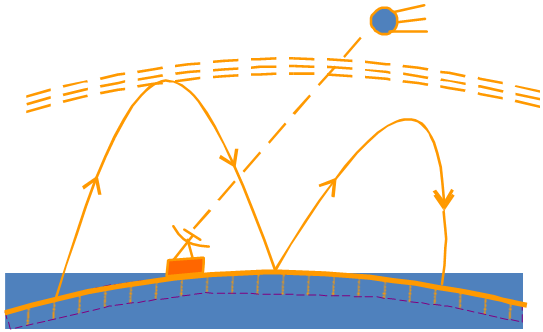
\includegraphics[width=6.5cm]{cosmicwindow.png}
\end{frame}

\begin{frame}{微波的特点}
  \begin{enumerate}
    \resume
    \item 计算机的运算次数进入十亿次,其频率也是微波频率。超高速集成电路的互耦也是微波互耦问题,因此,微波的研究已进入集成电路和计算机。
    \item 微波研究方法主要有两种:场论的研究方法和网络的研究方法。这也是本门课程要学习的重要方法。其中场论方法的基础是本征模理论。网络方法的基础是广义传输线理论。
  \end{enumerate}
\end{frame}

\subsection{2\quad 微波的应用}
\begin{frame}{微波技术的应用}
  \begin{tikzpicture}
    \node[draw,
    %fill=blue,
    minimum width=2cm,
    minimum height=1.2cm]
    (sum) at (0,0){微波应用};
  \end{tikzpicture}
\end{frame}

\begin{frame}{微波技术的发展}

\end{frame}

\subsection{3\quad 本课程内容}
\begin{frame}{本课程内容}
  \begin{columns}
    \begin{column}{0.15\linewidth}
      \begin{enumerate}
        \item 引论
        \saveenum
      \end{enumerate}
    \end{column}
    \begin{column}{0.35\linewidth}
      \textcolor{blue}{均匀传输线和波导理论基础}\\
      \textcolor{blue}{微波电路元件}
    \end{column}
    \begin{column}{0.5\linewidth}
      \begin{enumerate}
        \resume
        \item \textbf{传输线理论}
        \item \textbf{规则金属波导}
        \item \textbf{微波集成电路}
        \item 毫米波介质波导与光波导
        \item \textbf{微波网络基础}
        \item \textbf{微波谐振器}
        \item \textbf{常用微波器件}
        \item 微波铁氧体元件
      \end{enumerate}
    \end{column}
  \end{columns}
\end{frame}

\begin{frame}{微波技术的研究方法}

\end{frame}

\subsection{4\quad 导行波及其传输特性}
\begin{frame}{基本概念}
  \begin{enumerate}
    \item \textbf{导行系统(Guided system)}
    \saveenum
    \\约束或导引电磁能量定向传播\\
    作用:\\
    \begin{itemize}
      \item 无辐射损耗的将电磁波从一处传到另一处
      \item 设计成微波元件:滤波器、阻抗变换器、定向耦合器等。
    \end{itemize}
    微波电路是一种由各种导行系统构成的导行电磁波电路
  \end{enumerate}

\end{frame}

\begin{frame}{导行系统结构}
  %\begin{figure}
    \centering
    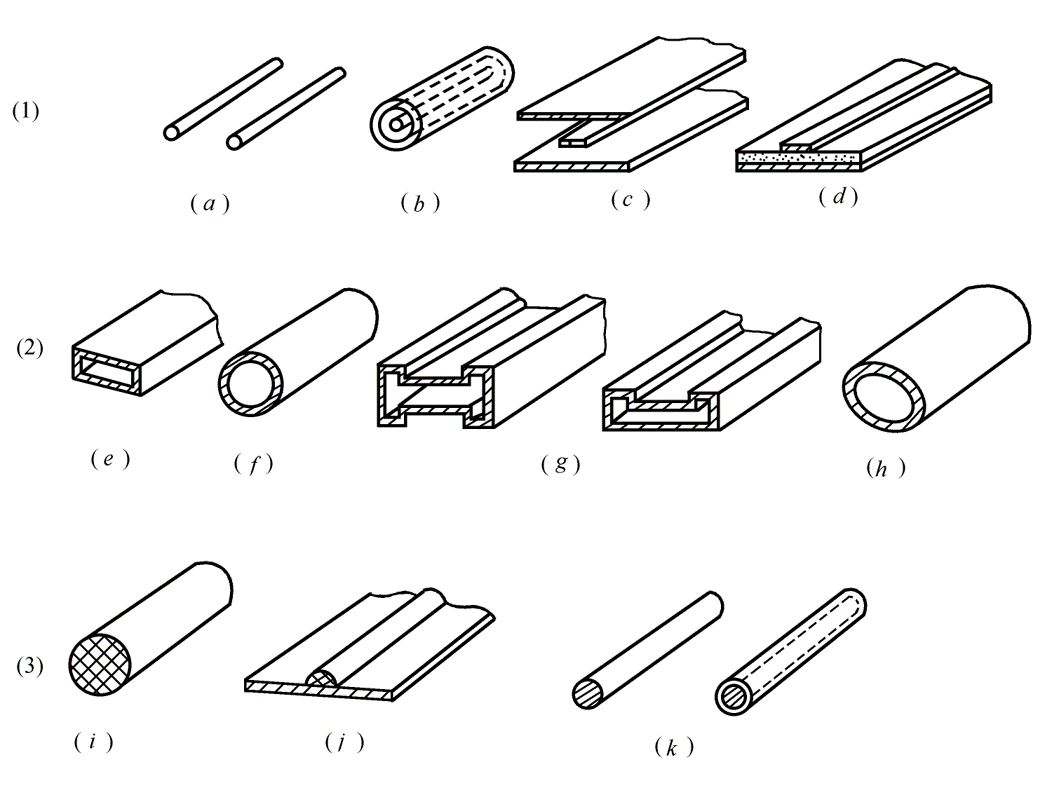
\includegraphics[width=9cm]{guidesystem.png}
  %\end{figure}
\end{frame}

\begin{frame}{基本概念}
  \begin{enumerate}
    \resume
    \item \textbf{导行波(Guided Wave)}
    \\沿导行系统定向传播的电磁波(导波)
    \\\textbf{TEM波}\quad 横电磁波 —— 各种传输线 电磁能量约束或限制在导体之间的空间内沿其轴向传播
    \\\textbf{TE/TM波}\quad 横电/横磁波 —— 封闭金属波导 电磁能量完全限制在金属管内沿轴向传播
    \\\textbf{表面波} —— 开波导 电磁能量约束在波导结构的周围(波导内和波导表面附近)沿轴向传播
    \saveenum
  \end{enumerate}
\end{frame}

\begin{frame}{基本概念}
  \begin{enumerate}
    \resume
    \item \textbf{导模(Guided mode)}
    \\导行波的模式(传输模)
    \\ *在导行系统横截面上的电磁场呈驻波分布,且完全确定的,与位置和频率无关
    \\ *导模是离散的,当频率一定时,每个导模具有唯一的传播常数
    \\ *导模之间相互正交,彼此独立,互不耦合
    \\ *具有截止特性,截止条件和截止波长因导行系统和模式而异
    \item \textbf{规则导行系统(Regular guided system)}
    \\无限长笔直导行系统,其横截面尺寸、媒质分布、结构材料、边界条件沿轴向均不变化
  \end{enumerate}
\end{frame}

\begin{frame}{导波场的分析}
  在\textbf{均匀}、\textbf{无耗}、\textbf{各向同性}、\textbf{无源}导行系统中
  \begin{columns}
    \begin{column}{0.5\linewidth}
      \begin{empheq}[box=\widefbox]{align*}
        &\nabla\times\vec E=-\frac{\partial \vec B}{\partial t}\\
        &\nabla\times\vec H=\vec{J} +\frac{\partial \vec D}{\partial t}\\
        &\nabla\cdot\vec{D}=\rho\\
        &\nabla\cdot\vec{B}=0
      \end{empheq}
      设导波沿$z$向传播,坐标$z$与横向坐标无关
    \end{column}
    \begin{column}{0.5\linewidth}
      \flushright
      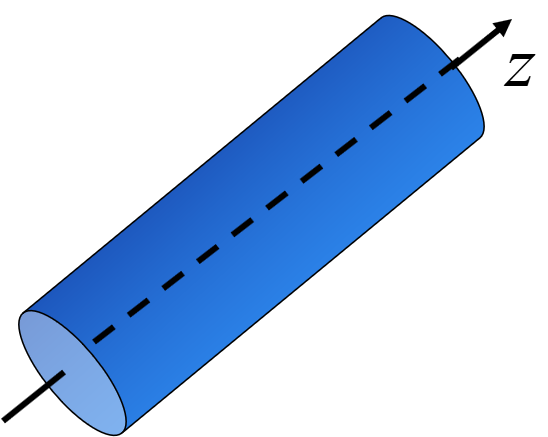
\includegraphics[width=4cm]{zuobiao.png}
      \begin{align*}
        & \nabla=\nabla_{t}+\hat z \partial / \partial z\\
        & \vec E=\vec E_{t}+\hat z E_{z}\\
        & \vec H=\vec H_{t}+\hat z H_{z}
      \end{align*}
    \end{column}
  \end{columns}
\end{frame}

\newcommand{\mtikzmark}[1]{\tikz[overlay,remember picture]\node(#1){};}
\tikzset{mylabel/.style={align=center,fill=blue!10,font=\footnotesize}}
%\mytlabel[options]{start.mark}{end.mark}{text}
\newcommand\mytlabel[4][]{%
\tikz[overlay,remember picture]
{\draw[->]([yshift=-10pt]#2.north) -- node[mylabel,#1]{#4}([yshift=6pt]#3.north);}
}
\begin{frame}{导波场的分析}
  \begin{columns}
    \begin{column}{0.45\linewidth}
      \begin{empheq}[box=\widefbox]{align*}
        %\tikzmarkin{c}(0.05,-0.6)(-0.05,0.65)
        & \nabla_t\times\vec{H_{t}}=j\omega\epsilon\hat{z}E_{z} \\
        & \nabla_t\times\hat{z}H_{z}+\hat{z}\times\frac{\partial\vec{H_{t}}}{\partial z}
        = \mtikzmark{a}j\omega\epsilon\vec{E_{t}}
      \end{empheq}
      %$$\times j\omega\mu$$
    \end{column}
    \begin{column}{0.5\linewidth}
      \begin{empheq}[box=\widefbox]{align*}
        & \nabla_t\times\vec E_{t}=-j\omega\mu\hat{z} H_{z} \\
        & \nabla_t\times \hat z E_{z}+\hat{z}\times\mtikzmark{c}\frac{\partial\vec{E_{t}}}{\partial z}
        = -j\omega\mu\vec{H_t}
      \end{empheq}
    \end{column}
  \end{columns}
  \begin{flalign*}
      & j\omega\mu\hat{z}\times\frac{\partial \vec{H_{t}}}{\partial z}=\mtikzmark{b}-j\omega\mu\nabla_{t}\times\hat{z}H_{z}-\omega^{2}\mu\epsilon\vec{E_{t}} &
  \end{flalign*}
  \begin{flalign*}
    && -j\omega\mu\hat{z}\times\frac{\partial \vec{H_{t}}}{\partial z}=\hat{z}\times\frac{\partial}{\partial z} \left(\nabla_{t}\times\hat{z}E_{z}\right)+\hat{z}\times\mtikzmark{d}\frac{\partial}{\partial z} \left(\hat{z} \times \frac{\partial \vec{E_{t}}}{\partial z} \right)
  \end{flalign*}
  % draw arrow with text from specified position to another
  \mytlabel{a}{b}{$\times j\omega\mu$}
  \mytlabel{c}{d}{$\hat{z}\times\frac{\partial}{\partial z}$}
\end{frame}

\begin{frame}{导波场的分析}
  \begin{empheq}[box=\widefbox]{align*}
    \left( k^{2}+\frac{\partial^{2}}{\partial z^{2}} \right)\vec{E_{t}}=\frac{\partial}{\partial z}\nabla_{t}E_{z}-j\omega\mu\nabla_{t}\times\hat{z}H_{z}
  \end{empheq}
  \begin{empheq}[box=\widefbox]{align*}
    \left( k^{2}+\frac{\partial^{2}}{\partial z^{2}} \right)\vec{H_{t}}=\frac{\partial}{\partial z}\nabla_{t}H_{z}-j\omega\epsilon\nabla_{t}\times\hat{z}E_{z}
  \end{empheq}
  在规则导行系统中,导波场的\textbf{横向分量}可用\textbf{纵向分量}完全确定。\\上面公式中$k^{2}=\omega^{2}\mu\epsilon$
\end{frame}

\begin{frame}{导波场的分析}
  \begin{empheq}[box=\widefbox]{align*}
    & \nabla^{2}\vec{E}+k^{2}\vec{E}=0\\
    & \nabla^{2}\vec{H}+\mtikzmark{a}k^{2}\vec{H}=0
  \end{empheq}
  \begin{columns}
    \begin{column}{0.45\linewidth}
      \begin{empheq}[box=\widefbox]{align*}
        & \nabla^{2}E_{z}+\mtikzmark{b}k^{2}E_{z}=0\\
        & \nabla^{2}H_{z}+\mtikzmark{d}k^{2}H_{z}=0
      \end{empheq}
    \end{column}
    \begin{column}{0.45\linewidth}
      \begin{empheq}[box=\widefbox]{align*}
        & \nabla^{2}\vec{E}_{t}+\mtikzmark{c}k^{2}\vec{E}_{t}=0\\
        & \nabla^{2}\vec{H}_{t}+k^{2}\vec{H}_{t}=0
      \end{empheq}
    \end{column}
  \end{columns}
  \flushright
  \begin{empheq}[box=\widefbox]{align*}
    \left( \nabla^{2}_{t}+\frac{\partial^{2}}{\partial z^{2}}\right)
    \left\{\begin{aligned}
      \mtikzmark{e}E_{z}(z,t)\\H_{z}(z,t)
    \end{aligned}\right\}
    +k^{2}
    \left\{\begin{aligned}
      E_{z}(z,t)\\H_{z}(z,t)
    \end{aligned}\right\}
    =0
  \end{empheq}
  \mytlabel{a}{b}{纵向场}
  \mytlabel{a}{c}{横向场}
  \mytlabel{d}{e}{Helmholtz Equation}
\end{frame}

\begin{frame}{导波场的分析}
  \begin{empheq}[box=\widefbox]{align*}
    \left( \nabla^{2}_{t}+\frac{\partial^{2}}{\partial z^{2}}\right)
    \left\{\begin{aligned}
      \mtikzmark{e}E_{z}(z,t)\\H_{z}(z,t)
    \end{aligned}\right\}
    +k^{2}
    \left\{\begin{aligned}
      E_{z}(z,t)\\H_{z}(z,t)
    \end{aligned}\right\}
    =0
  \end{empheq}
  \begin{enumerate}
    \item \textbf{分离变量法}\\
    令$E_{z}(z,t)=Z(z)E_{0z}(t)$ \\
    \begin{align*}
      \frac{\nabla_{t}^{2}E_{0z}(t)}{E_{0z}(t)}+\frac{d^{2}Z(z)/dz^{2}}{Z(z)}=-k^{2}
    \end{align*}
    \begin{columns}
      \begin{column}{0.3\linewidth}
        分离变量常数: $k_{c}$和$\beta$
      \end{column}
      \begin{column}{0.6\linewidth}
        \begin{empheq}[box=\widefbox]{align*}
          & d^{2}Z(z)/dz^{2}+\beta^{2}Z(z)=0 \\
          & \nabla_{t}^{2}E_{0z}(t)+k_{c}^{2}E_{0z}(t)=0
        \end{empheq}
        \flushright————本征值方程
      \end{column}
    \end{columns}
    \saveenum
  \end{enumerate}
\end{frame}

\begin{frame}{导波场的分析}
  \begin{enumerate}
    \resume
    \item \textbf{色散关系}
    \begin{columns}
      \begin{column}{0.55\linewidth}
        \begin{empheq}[box=\widefbox]{align*}
          & k^{2}=k_{c}^{2}+\beta^{2}\\
          & \beta=\sqrt{k^{2}-k_{c}^{2}}=k\sqrt{1-(k_{c}/k)^{2}}
        \end{empheq}
      \end{column}
      \begin{column}{0.4\linewidth}
        \raggedright
        $k^{2}=\omega^{2}\mu\epsilon$\\  $\beta$:导波的传播常数或相移常数
      \end{column}
    \end{columns}
    $$d^{2}Z(z)/dz^{2}+\beta^{2}Z(z)=0$$
    %\flushleft
    解:
    \begin{empheq}[box=\widefbox]{align*}
      Z(z)=A_{1}exp(-j\beta z)+A_{2}exp(j\beta z)
    \end{empheq}
    \textbf{规则导行系统中沿正$z$方向传播的导波纵向场分量}\\
    \begin{align*}
      E_{z}(t,z)=E_{0z}(t)exp(-j\beta z)\\
      H_{z}(t,z)=H_{0z}(t)exp(-j\beta z)
    \end{align*}
    \saveenum
  \end{enumerate}
\end{frame}

\begin{frame}{导波场的分析}
  \begin{enumerate}
    \resume
    \item 本征值方程
    \begin{empheq}[box=\widefbox]{align*}
      \nabla_{t}^{2}E_{0z}(t)+k_{c}^{2}E_{0z}(t)=0
    \end{empheq}
    $k_{c}$:在特定边界条件下的本征值,称为导波的横向截止波数\\
    $k_{c}\neq 0$
    \saveenum
  \end{enumerate}
\end{frame}

\begin{frame}{导波场的分析}
  \begin{enumerate}
    \resume
    \item 横-纵向场的关系
    \begin{empheq}[box=\widefbox]{align*}
      \left( k^{2}+\frac{\partial_{2}}{\partial z^{2}}\right)\vec{E}_{t}=\frac{\partial}{\partial z}\nabla_{t}E_{z}-j\omega\mu\nabla_{t}\times\hat{z}H_{z}\\
      \left( k^{2}+\frac{\partial_{2}}{\partial z^{2}}\right)\vec{H}_{t}=\frac{\partial}{\partial z}\nabla_{t}H_{z}-j\omega\epsilon\nabla_{t}\times\hat{z}E_{z}
    \end{empheq}
    \begin{columns}
      \begin{column}{0.6\linewidth}
        \begin{empheq}[box=\widefbox]{align*}
          \vec{E}_{t}=\frac{-j\beta}{k_{c}^{2}}\left[\nabla_{t}E_{z}+Z_{h}\nabla_{t}H_{z}\times\hat{z}\right]\\
          \vec{H}_{t}=\frac{-j\beta}{k_{c}^{2}}\left[\nabla_{t}H_{z}+Y_{e}\hat{z}\times\nabla_{t}E_{z}\right]
        \end{empheq}
      \end{column}
      \begin{column}{0.4\linewidth}
        \begin{align*}
          Z_{h}=\sqrt{\frac{\mu}{\epsilon}}\frac{k}{\beta}\\
          Y_{e}=\sqrt{\frac{\epsilon}{\mu}}\frac{k}{\beta}
        \end{align*}
      \end{column}
    \end{columns}
    \saveenum
  \end{enumerate}
\end{frame}

\begin{frame}{导波场的分析}
  \begin{enumerate}
    \resume
    \item 导波的种类\\
    \begin{block}{横磁波(TM)或电(E)波——$H_{z}=0$}
      \begin{empheq}[box=\widefbox]{align*}
        \vec{E}_{t}^{e}=\frac{-j\beta}{k_{c}^{2}}\nabla_{t}E_{z}\qquad
        \vec{H}_{t}^{e}=\frac{-j\beta}{k_{c}^{2}}Y_{e}\hat{z}\times\nabla_{t}E_{z}
      \end{empheq}
    \end{block}
    \begin{block}{横电波(TE)或磁(H)波——$E_{z}=0$}
      \begin{empheq}[box=\widefbox]{align*}
        \vec{E}_{t}^{h}=\frac{-j\beta}{k_{c}^{2}}Z_{h}\nabla_{t}H_{z}\times\hat{z}\qquad
        \vec{H}_{t}^{h}=\frac{-j\beta}{k_{c}^{2}}\nabla_{t}H_{z}
      \end{empheq}
    \end{block}
    导行系统横向为调谐(振动)解形式$k_{c}^{2}>0$,$k^{2}>\beta^{2}$;$\beta=k\cdot\sqrt{1-\left(\frac{k_{c}}{k}\right)^{2}}$ 相速$v_{p}>c/\sqrt{\epsilon_{r}}$快波,有色散性,且需满足$k_{c}<k$才能传播。
  \end{enumerate}
\end{frame}

\begin{frame}{导波场的分析}
  \begin{block}{横电磁波(TEM)——$E_{z}=H_{z}=0$}
    %\begin{flalign*}
      $$ \because E_{t}\neq 0,H_{t}\neq 0 $$
    %\end{flalign*}
    以及
    \begin{align*}
      & \vec{E}_{t}=\frac{-j\beta}{k_{c}^{2}}[\nabla_{t}E_{z}+Z_{h}\nabla_{t}H_{z}\times\hat{z}]\\
      & \vec{H}_{t}=\frac{-j\beta}{k_{c}^{2}}[\nabla_{t}H_{z}+Y_{e}\hat{z}\times\nabla_{t}E_{z}]
    \end{align*}
    $$\left(\frac{0}{0}\right)形式\Longrightarrow k_{c}=0 \qquad k^{2}=k_{c}^{2}+\beta^{2}\Longrightarrow \beta=k $$
  \end{block}
\end{frame}

\begin{frame}{导波场的分析}
  又由$\nabla_{t}\times\vec{E}_{t}=-j\omega\mu\hat{z}H_{z}$\qquad$\nabla_{t}\times\vec{H}_{t}=j\omega\epsilon\hat{z}E_{z}$
\end{frame}

\begin{frame}{导波场的分析}

\end{frame}

\begin{frame}{导行波的一般传输特性}

\end{frame}

\begin{frame}{导行波的一般传输特性}

\end{frame}

\begin{frame}{导行波的一般传输特性}

\end{frame}

\begin{frame}{导行波的一般传输特性}

\end{frame}

\end{document}

%\section{第二章\quad 传输线理论}

\begin{frame}{传输线理论}
 \begin{itemize}
  \item \textbf{传输线理论,一维分布参数电路理论,微波电路设计和计算的理论基础。}
  \item \textbf{传输线理论,电路理论与场的理论之间起着桥梁的作用。}
 \end{itemize}
\end{frame}

\subsection{传输线方程}
\begin{frame}{传输线方程}
 \begin{enumerate}
  \item 传输线的电路模型
 \end{enumerate}
 \centering
 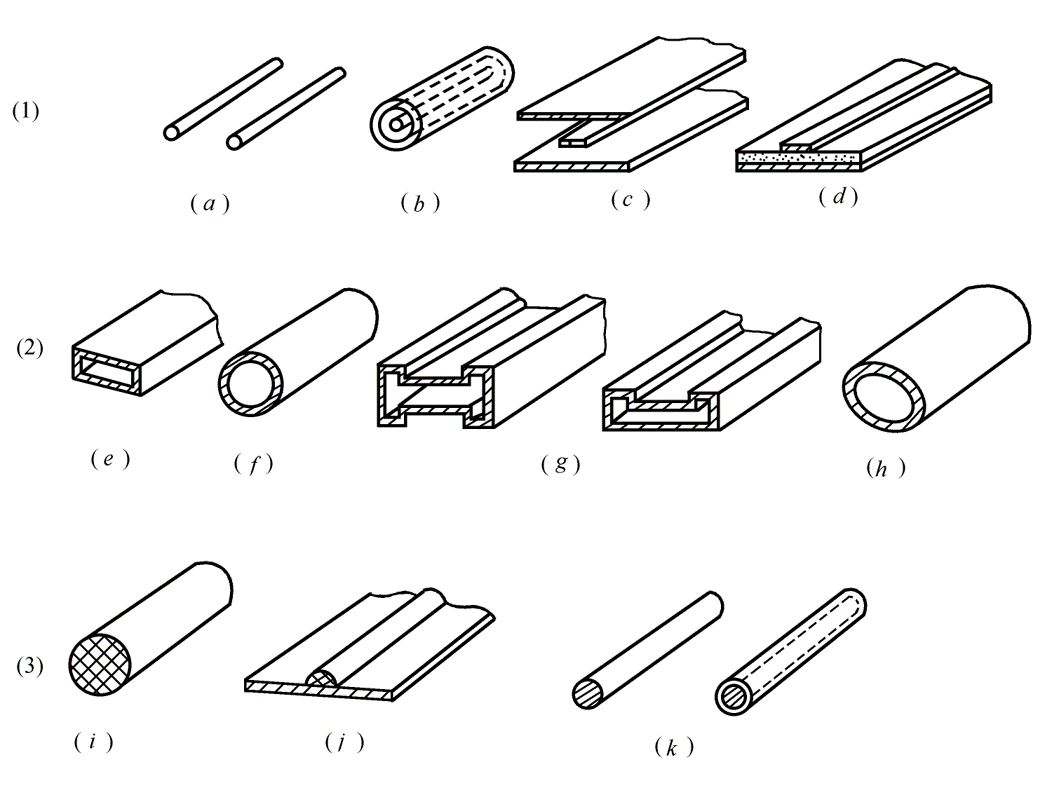
\includegraphics[width=9cm]{guidesystem.png}
 \saveenum
\end{frame}

\begin{frame}{传输线方程}
 \textbf{传输线}是以TEM导模的方式传送电磁波能量或信号的导行系统,其横向尺寸远小于其上工作波长。\\
 \textbf{传输线}有\textbf{长线}和\textbf{短线}之分。所谓长线是指传输线的几何长度与线上传输电磁波的波长比值(电长度)可相比拟,反之称为短线。\\
 \begin{align*}
  \text{长线}\Longrightarrow\text{分布参数电路} \\
  \text{短线}\Longrightarrow\text{集中参数电路} \\
  \text{分界线:}\widefbox{$l/\lambda\geq 0.05$}
 \end{align*}
 当频率提高到微波波段时,这些分布效应不可忽略,所以微波传输线是一种\textbf{分布参数电路}。这导致传输线上的电压和电流是随时间和空间位置而变化的二元函数。
\end{frame}

\begin{frame}{传输线方程}
 根据传输线上的分布参数是否均匀分布,可将其分为均匀传输线和不均匀传输线。我们可以把均匀传输线分割成许多小的微元段$dz(dz<<\lambda)$,这样每个微元段可以看作集中参数电路,用一个$\Gamma$型网络来等效。于是整个传输线可等效成无穷多个$\Gamma$型网络的级联。\\
 \centering
 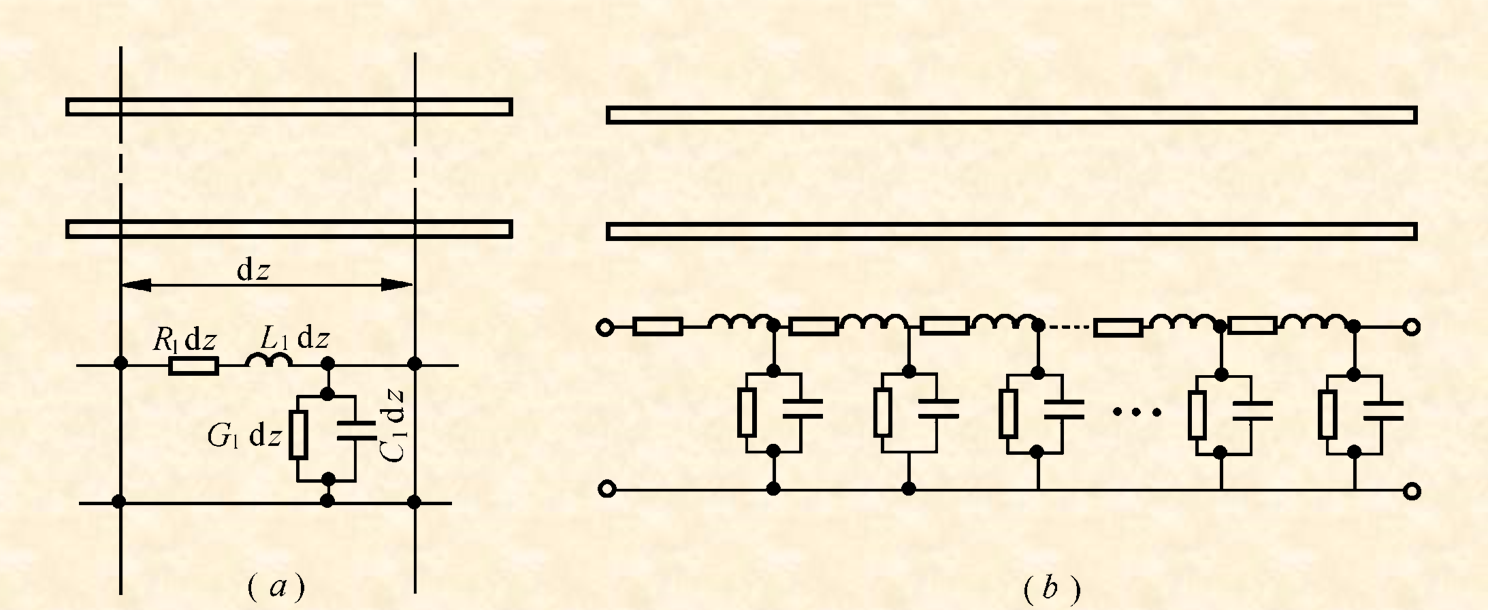
\includegraphics[width=9cm]{transmissionline1.png}
\end{frame}

\begin{frame}{传输线方程}
 双导线、同轴线和平行线传输线的分布参数\\
 \centering
 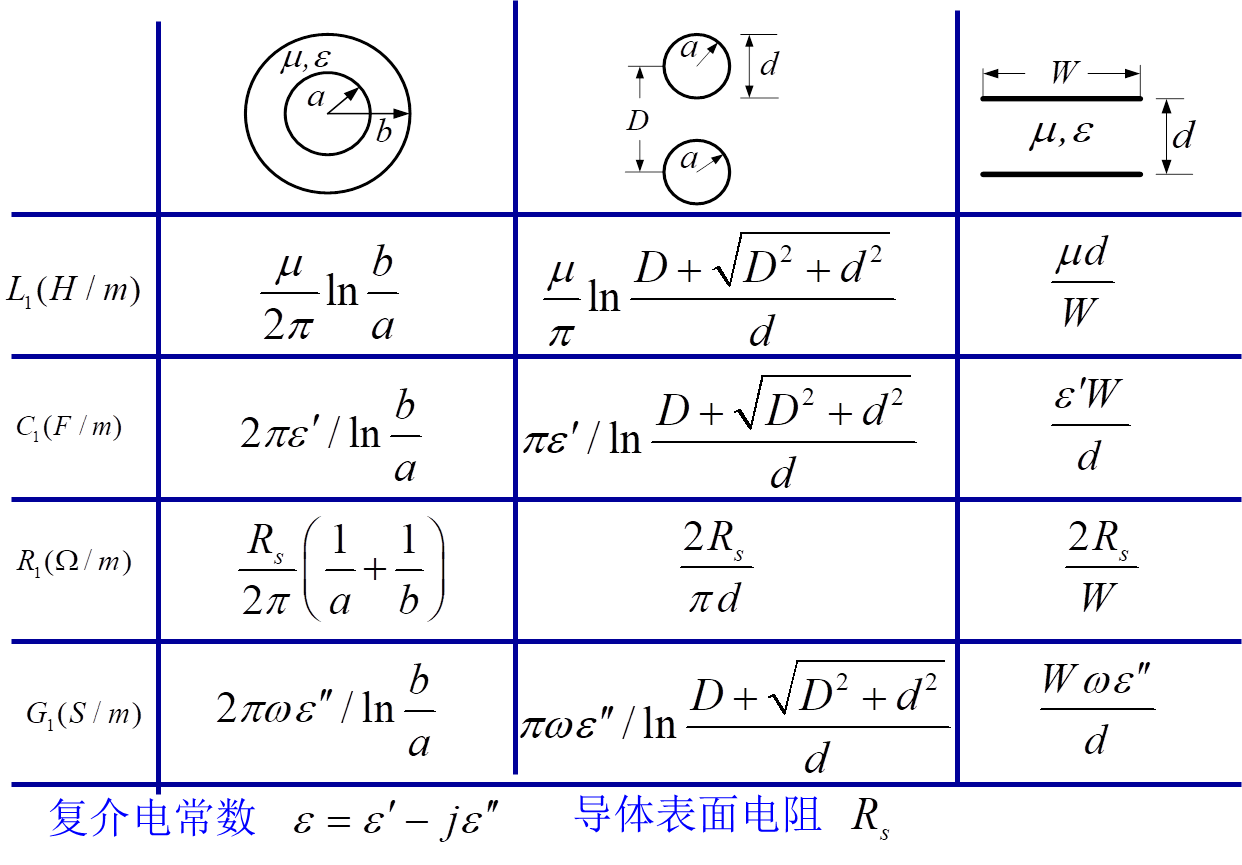
\includegraphics[width=9cm]{tmlineparas.png}
\end{frame}

\begin{frame}{传输线方程}
 \begin{enumerate}
  \resume
  \item 传输线方程\\
        \begin{itemize}
         \item 一般传输线方程或电报方程\\
               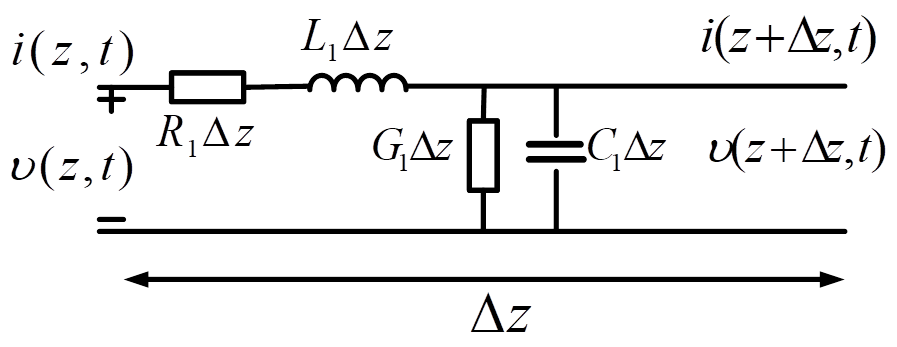
\includegraphics[width=6cm]{transmissionline2.png}
        \end{itemize}
        \saveenum
 \end{enumerate}
 \flushleft
 \fbox{$ v(z+\Delta z,t)=v(z,t)+\frac{\partial v(z,t)}{\partial z}\Delta z $}
 \flushright
 \fbox{$ i(z+\Delta z,t)=i(z,t)+\frac{\partial i(z,t)}{\partial z}\Delta z $}\\
 \begin{align*}
  f(x)=f(x_{0})+f^{'}(x_{0})(x-x_{0})  +\frac{f^{''}(x_{0})}{2!}(x-x_{0})^{2}+\ldots \\
  +\frac{f^{n}(x_{0})}{n!}(x-x_{0})^{n}+R_{n}(x)
 \end{align*}
\end{frame}

\begin{frame}{传输线方程}
 \centering
 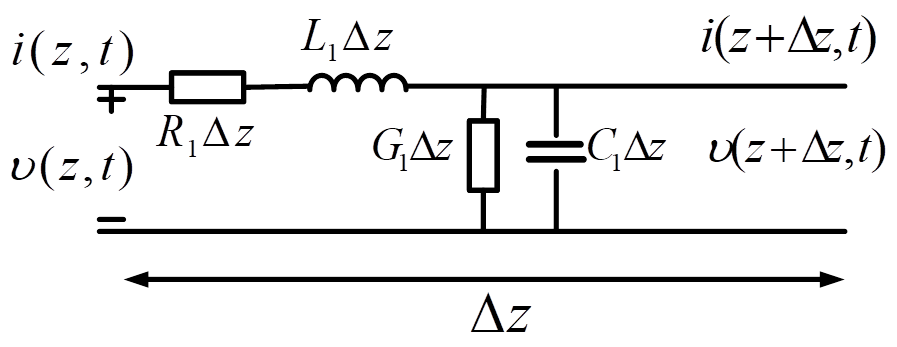
\includegraphics[width=7cm]{transmissionline2.png}
 \flushleft
 线元$\Delta z$上的电压、电流的变化为:
 \begin{empheq}[box=\widefbox]{align*}
  v(z,t)-v(z+\Delta z,t)=-\frac{\partial v(z,t)}{\partial z}\Delta z\\
  i(z,t)-i(z+\Delta z,t)=-\frac{\partial i(z,t)}{\partial z}\Delta z
 \end{empheq}
\end{frame}

\begin{frame}{传输线方程}
 \centering
 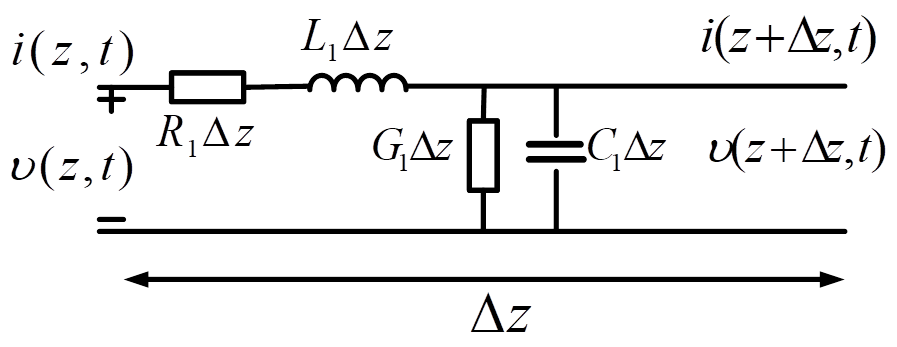
\includegraphics[width=7cm]{transmissionline2.png}
 \flushleft
 线元$\Delta z$上应用基尔霍夫定律,可得:
 \begin{empheq}[box=\widefbox]{align*}
  -\frac{\partial v(z,t)}{\partial z}\Delta z=R_{1}\Delta z\cdot i(z,t)+L_{1}\Delta z\cdot\frac{\partial i(z,t)}{\partial t}\\
  -\frac{\partial i(z,t)}{\partial z}\Delta z=G_{1}\Delta z\cdot v(z,t)+C_{1}\Delta z\cdot\frac{\partial v(z,t)}{\partial t}
 \end{empheq}
\end{frame}

\begin{frame}{传输线方程}
 \begin{empheq}[box=\widefbox]{align*}
  -\frac{\partial v(z,t)}{\partial z}\Delta z=R_{1}\Delta z\cdot i(z,t)+L_{1}\Delta z\cdot\frac{\partial i(z,t)}{\partial t}\\
  -\frac{\partial i(z,t)}{\partial z}\Delta z=G_{1}\Delta z\cdot v(z,t)+C_{1}\Delta z\cdot\frac{\partial v(z,t)}{\partial t}
 \end{empheq}
 \flushleft
 令$\Delta z \rightarrow 0$
 \begin{empheq}[box=\widefbox]{align*}
  \frac{\partial v(z,t)}{\partial z}=-R_{1}\cdot i(z,t)-L_{1}\cdot\frac{\partial i(z,t)}{\partial t}\\
  \frac{\partial i(z,t)}{\partial z}=-G_{1}\cdot v(z,t)-C_{1}\cdot\frac{\partial v(z,t)}{\partial t}
 \end{empheq}
 \centering
 \textbf{一般传输线方程、电报方程}
\end{frame}

\begin{comment}
\newcommand{\mtikzmark}[1]{\tikz[overlay,remember picture]\node(#1){};}
\tikzset{mylabel/.style={align=center,fill=blue!10,font=\footnotesize}}
%\mytlabel[options]{start.mark}{end.mark}{text}
\newcommand\mytlabel[4][]{%
 \tikz[overlay,remember picture]
 {\draw[->]([yshift=-10pt]#2.north) -- node[mylabel,#1]{#4}([yshift=6pt]#3.north);}
}
\end{comment}

\begin{frame}{传输线方程}
 \begin{itemize}
  \item 时谐均匀传输线方程
 \end{itemize}
 \begin{empheq}[box=\widefbox]{align*}
  \frac{\partial v(z,t)}{\partial z}=-R_{1}\cdot i(z,t)-L_{1}\cdot\frac{\partial i(z,t)}{\partial t}\\
  \frac{\partial i(z,t)}{\partial z}=-G_{1}\cdot v(z,t)-C_{1}\cdot\frac{\partial v(z,t)}{\partial t}
 \end{empheq}
 \begin{columns}
  \begin{column}{0.5\linewidth}
   \begin{empheq}[box=\widefbox]{align*}
    v(z,t)=Re\left[V(z)e^{j\omega t}\right]\\
    i(z,t)=Re\left[I(z)e^{j\omega t}\right]
   \end{empheq}
  \end{column}
  \begin{column}{0.5\linewidth}
   分布参数:$R_{1}$,$L_{1}$,$C_{1}$,$G_{1}$不随位置变化
  \end{column}
 \end{columns}
\end{frame}

\begin{frame}{传输线方程}
 \begin{empheq}[box=\widefbox]{align*}
  \frac{dV(z)}{dz}=-(R_{1}+j\omega L_{1})I(z)=-Z_{1}I(z)\\
  Z_{1}=R_{1}+j\omega L_{1} \text{:单位长度串联阻抗}
 \end{empheq}
 \begin{empheq}[box=\widefbox]{align*}
  \frac{dI(z)}{dz}=-(G_{1}+j\omega C_{1})V(z)=-Y_{1}V(z)\\
  Y_{1}=G_{1}+j\omega C_{1} \text{:单位长度并联导纳}
 \end{empheq}
 对$z$再微商
 \begin{align*}
  \frac{d^2}{dz^2}\left\{
  \begin{aligned}
   V(z) \\I(z)
  \end{aligned}
  \right\}-\gamma^2
  \left\{\begin{aligned}
          V(z) \\I(z)
         \end{aligned}\right\}=0
 \end{align*}
 \textbf{电压传播常数}:\fbox{$\gamma=\sqrt{Z_{1}Y_{1}}=\sqrt{(R_{1}+j\omega L_{1})(G_{1}+j\omega C_{1})}$}
\end{frame}

\begin{frame}{传输线方程}
 \begin{itemize}
  \item 时谐传输线方程电压、电流通解
 \end{itemize}
 电压:
 \begin{empheq}[box=\widefbox]{align*}
  V(z)=A_{1}e^{-\gamma z}+A_{2}e^{\gamma z}
 \end{empheq}
 电流:
 \begin{empheq}[box=\widefbox]{align*}
  I(z)=-\frac{1}{R_{1}+j\omega L_{1}}\frac{dV(z)}{dz}=\frac{1}{Z_{0}}(A_{1}e^{-\gamma z}-A_{2}e^{\gamma z})
 \end{empheq}
 $$\gamma=\sqrt{Z_{1}Y_{1}}=\sqrt{(R_{1}+j\omega L_{1})(G_{1}+j\omega C_{1})}$$
 \textbf{特性阻抗}:
 \begin{empheq}[box=\widefbox]{align*}
  Z_{0}=\sqrt{\frac{R_{1}+j\omega L_{1}}{G_{1}+j\omega C_{1}}}
 \end{empheq}
\end{frame}

\begin{frame}{传输线方程}
 \begin{itemize}
  \item 传输线方程的边界条件和解
 \end{itemize}
 \begin{columns}
  \begin{column}{0.35\linewidth}
   端接条件确定常数:\\
   终端条件\\
   始端条件\\
   信号源和负载条件
  \end{column}
  \begin{column}{0.65\linewidth}
   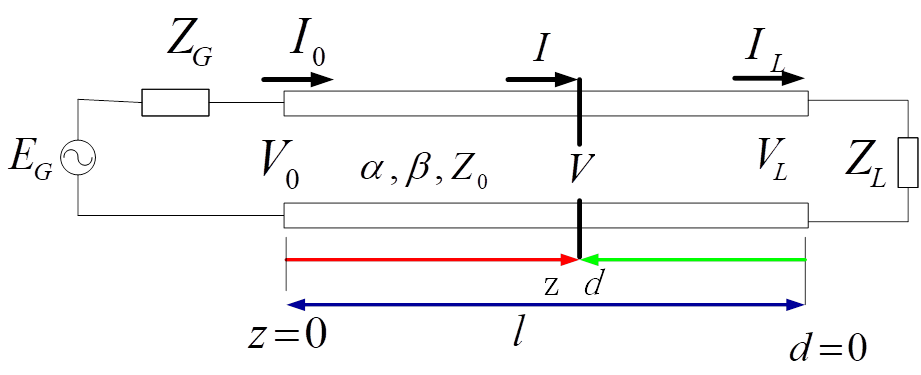
\includegraphics[width=6cm]{tmlineboundary.png}
  \end{column}
 \end{columns}
 \textbf{终端条件}解:
 \begin{columns}
  \begin{column}{0.5\linewidth}
   \begin{empheq}[box=\widefbox]{align*}
    V(z)=A_{1}e^{-\gamma z}+A_{2}e^{\gamma z}
   \end{empheq}
  \end{column}
  \begin{column}{0.5\linewidth}
   \begin{empheq}[box=\widefbox]{align*}
    I(z)=(A_{1}e^{-\gamma z}-A_{2}e^{\gamma z})/Z_{0}
   \end{empheq}
  \end{column}
 \end{columns}
 \begin{empheq}[box=\widefbox]{align*}
  V(l)=V_{L}=A_{1}e^{-\gamma l}+A_{2}e^{\gamma l}\\
  I(l)=I_{L}=\frac{1}{Z_{0}}(A_{1}e^{-\gamma l}-A_{2}e^{\gamma l})
 \end{empheq}
\end{frame}

\begin{frame}{传输线方程}
 \begin{empheq}[box=\widefbox]{align*}
  A_{1}=\frac{V_{L}+I_{L}Z_{0}}{2}e^{\gamma l},A_{2}=\frac{V_{L}-I_{L}Z_{0}}{2}e^{-\gamma l}
 \end{empheq}
 代入:
 \begin{columns}
  \begin{column}{0.45\linewidth}
   \begin{empheq}[box=\widefbox]{align*}
    V(z)=A_{1}e^{-\gamma z}+A_{2}e^{\gamma z}
   \end{empheq}
  \end{column}
  \begin{column}{0.45\linewidth}
   \begin{empheq}[box=\widefbox]{align*}
    I(z)=(A_{1}e^{-\gamma z}-A_{2}e^{\gamma z})/Z_{0}
   \end{empheq}
  \end{column}
 \end{columns}
 对于终端边界条件场合,我们常采用$d$(终端出发)坐标系$d$,换坐标\fbox{$d=l-z$}
 \begin{empheq}[box=\widefbox]{align*}
  V(d)=\frac{V_{L}+I_{L}Z_{0}}{2}e^{\gamma d}+\frac{V_{L}-I_{L}Z_{0}}{2}e^{-\gamma d}=V^{+}(d)+V^{-}(d)\\
  I(d)=\frac{V_{L}+I_{L}Z_{0}}{2Z_{0}}e^{\gamma d}-\frac{V_{L}-I_{L}Z_{0}}{2Z_{0}}e^{-\gamma d}=I^{+}(d)+I^{-}(d)
 \end{empheq}
\end{frame}

\begin{frame}{传输线方程}
 \begin{empheq}[box=\widefbox]{align*}
  V(d)=\frac{V_{L}+I_{L}Z_{0}}{2}e^{\gamma d}+\frac{V_{L}-I_{L}Z_{0}}{2}e^{-\gamma d}=V^{+}(d)+V^{-}(d)\\
  I(d)=\frac{V_{L}+I_{L}Z_{0}}{2Z_{0}}e^{\gamma d}-\frac{V_{L}-I_{L}Z_{0}}{2Z_{0}}e^{-\gamma d}=I^{+}(d)+I^{-}(d)
 \end{empheq}
 \begin{empheq}[box=\widefbox]{align*}
  V(d)=\frac{e^{\gamma d}+e^{-\gamma d}}{2}V_{L}+\frac{e^{\gamma d}-e^{-\gamma d}}{2}Z_{0}I_{L}\\
  I(d)=\frac{e^{\gamma d}+e^{-\gamma d}}{2}\frac{1}{Z_{0}}V_{L}+\frac{e^{\gamma d}-e^{-\gamma d}}{2}I_{L}
 \end{empheq}
 \begin{align*}
  \begin{bmatrix}
   V(d) \\I(d)
  \end{bmatrix}
  =
  \begin{bmatrix}
   \cosh\gamma d           & Z_{0}\sinh\gamma d \\
   Z_{0}^{-1}\sinh\gamma d & \cosh\gamma d
  \end{bmatrix}
  \begin{bmatrix}
   V_{L} \\I_{L}
  \end{bmatrix}
 \end{align*}
\end{frame}

\begin{frame}{传输线方程}
 \textbf{始端条件解}:已知始端电压和电流$V_{0},I_{0}$ \\
 \fbox{$V(z)=A_{1}e^{-\gamma z}+A_{2}e^{\gamma z}$}
 \fbox{$I(z)=(A_{1}e^{-\gamma z}-A_{2}e^{\gamma z})/Z_{0}$}\\
 \begin{columns}
  \begin{column}{0.3\linewidth}
   \begin{align*}
    V_{0}=A_{1}+A_{2} \\
    I_{0}=(A_{1}-A_{2})/Z_{0}
   \end{align*}
  \end{column}
  \begin{column}{0.1\linewidth}
   \centering
   $ \longrightarrow $
  \end{column}
  \begin{column}{0.6\linewidth}
   \begin{empheq}[box=\fbox]{align*}
    A_{1}=\frac{V_{0}+I_{0}Z_{0}}{2}\quad A_{2}=\frac{V_{0}-I_{0}Z_{0}}{2}
   \end{empheq}
  \end{column}
 \end{columns}
 \begin{empheq}[box=\widefbox]{align*}
  V(z)=\frac{V_{0}+I_{0}Z_{0}}{2}e^{-\gamma z}+\frac{V_{0}-I_{0}Z_{0}}{2}e^{\gamma z}\\
  I(z)=\frac{V_{0}+I_{0}Z_{0}}{2Z_{0}}e^{-\gamma z}+\frac{V_{0}-I_{0}Z_{0}}{2Z_{0}}e^{\gamma z}
 \end{empheq}
 \begin{align*}
  \begin{bmatrix}
   V(z) \\I(z)
  \end{bmatrix}
  =
  \begin{bmatrix}
   \cosh\gamma z            & -Z_{0}\sinh\gamma z \\
   -Z_{0}^{-1}\sinh\gamma z & \cosh\gamma z
  \end{bmatrix}
  \begin{bmatrix}
   V_{0} \\I_{0}
  \end{bmatrix}
 \end{align*}
\end{frame}

\begin{frame}{传输线方程}
 \textbf{信号源和负载条件解}:
 已知信号源电动势 $E_{G}$、
 内阻抗 $Z_{G}$、
 负载阻抗 $Z_{L}$
 \begin{empheq}[box=\widefbox]{align*}
  V(d)=\frac{E_{G}Z_{0}}{Z_{G}+Z_{0}}\cdot\frac{e^{-\gamma l}}{1-\Gamma_{L}\Gamma_{G}e^{-2\gamma l}}(e^{\gamma d}+\Gamma_{L}e^{-\gamma d})\\
  I(d)=\frac{E_{G}}{Z_{G}+Z_{0}}\cdot\frac{e^{-\gamma l}}{1-\Gamma_{L}\Gamma_{G}e^{-2\gamma l}}(e^{\gamma d}-\Gamma_{L}e^{-\gamma d})
 \end{empheq}
 \begin{align*}
  \Gamma_{L}=\frac{Z_{L}-Z_{0}}{Z_{L}+Z_{0}}\quad \Gamma_{G}=\frac{Z_{G}-Z_{0}}{Z_{G}+Z_{0}}\quad\text{反射系数}
 \end{align*}
\end{frame}

\begin{frame}{传输线方程}
 \begin{enumerate}
  \resume
  \item \textbf{传输线的特性参数}
        \begin{itemize}
         \item 特性阻抗
        \end{itemize}
        \begin{align*}
         Z_{0}=\sqrt{\frac{R_{1}+j\omega L_{1}}{G_{1}+j\omega C_{1}}}
        \end{align*}
        传输线上\textbf{行波}的电压与电流之比称为传输线的特性阻抗\\
        $$\text{无耗线}R_{1}=G_{1}=0\quad Z_{0}=\sqrt{\frac{L_{1}}{C_{1}}}$$\\
        微波低耗线$R_{1}<<\omega L_{1},G_{1}<<\omega C_{1}$\\
        $$Z_{0}=\sqrt{\frac{R_{1}+j\omega L_{1}}{G_{1}+j\omega C_{1}}}\approx\sqrt{\frac{L_{1}}{C_{1}}}\left[1+\frac{1}{2}\left(\frac{R_{1}}{j\omega L_{1}}-\frac{G_{1}}{j\omega C_{1}}\right)\right]$$
 \end{enumerate}
\end{frame}

\begin{frame}{传输线方程}
 \begin{itemize}
  \item \textbf{双导线特性阻抗}\\
        $$Z_{0}=120\ln\left[\frac{D}{d}+\sqrt{\left(\frac{D}{d}\right)^{2}-1}\right]$$
  \item \textbf{同轴线特性阻抗}\\
        $$Z_{0}=\frac{60}{\sqrt{\epsilon_{r}}}\ln\frac{b}{a}$$
  \item \textbf{平行板传输线特性阻抗}\\
        $$Z_{0}=\frac{d}{W}\eta$$
 \end{itemize}
\end{frame}

\begin{frame}{传输线方程}
 \begin{itemize}
  \item \textbf{传播常数}
 \end{itemize}
 描述导行波沿着导行系统传播过程中的\textbf{衰减和相位变化}的参数
 \begin{empheq}[box=\widefbox]{align*}
  \gamma = \sqrt{(R_{1}+j\omega L_{1})(G_{1}+j\omega C_{1})}=\alpha+j\beta
 \end{empheq}
 $\alpha$——衰减常数,单位$Np/m$或$dB/m$\quad $(1Np=8.686dB)$\\
 $\beta$——相位常数,单位$rad/m$\\
 \centering
 $\text{无耗线}\quad \alpha=0$\quad \fbox{$\beta=\omega\sqrt{L_{1}C_{1}}$}
\end{frame}

\begin{frame}{传输线方程}
 微波低耗线\quad$R_{1}<<\omega L_{1},G_{1}<<\omega C_{1}$
 \begin{align*}
  \gamma & =\sqrt{(R_{1}+j\omega L_{1})(G_{1}+j\omega C_{1})}=\alpha+j\beta                                                \\
         & =\sqrt{(j\omega)^{2}L_{1}C_{1}}\sqrt{\left(1+\frac{R_{1}}{j\omega L_{1}}\right)(1+\frac{G_{1}}{j\omega C_{1}})} \\
         & \approx\frac{1}{2}\left(R_{1}\sqrt{C_{1}/L_{1}}+G_{1}\sqrt{L_{1}/C_{1}}\right)+j\omega\sqrt{L_{1}C_{1}}
 \end{align*}
 \begin{columns}
  \begin{column}{0.65\linewidth}
   \begin{empheq}[box=\widefbox]{align*}
    \therefore\alpha=\frac{R_{1}}{2Z_{0}}+\frac{G_{1}Z_{0}}{2}=\alpha_{c}+\alpha_{d}
   \end{empheq}
   $\alpha_{c}$:分布电阻产生的导体衰减常数\\
   $\alpha_{d}$:漏电导产生的介质衰减常数
  \end{column}
  \begin{column}{0.35\linewidth}
   \begin{empheq}[box=\widefbox]{align*}
    \therefore\beta=\omega\sqrt{L_{1}C_{1}}
   \end{empheq}
   $\beta$:近似于无耗传输线的相位常数
  \end{column}
 \end{columns}
\end{frame}

\begin{frame}{传输线方程}
 对于TEM导波:\\
 $$k_{c}=0,\lambda_{c}=\infty$$\\
 其相速度为\\
 $$v_{p}=v=\frac{\omega}{\beta}=\frac{1}{\sqrt{L_{1}C_{1}}}$$\\
 波长为\\
 $$\lambda_{g}=\lambda=\frac{2\pi}{\beta}=\frac{v_{p}}{f}$$\\
 特性阻抗为\\
 $$Z_{0}=\sqrt{\frac{L_{1}}{C_{1}}}=\frac{1}{v_{p}C_{1}}=v_{p}L_{1}$$\\
 \textbf{传输线的特性阻抗可由单位长度分布电容或分布电感求得}
\end{frame}

\subsection{分布参数阻抗}
\begin{frame}{分布参数阻抗}
 \begin{itemize}
  \item 微波阻抗——由微波传输线上的电压和电流决定的,是\textbf{分布参数}阻抗。(低频传输线阻抗是\textbf{集中参数}阻抗)
  \item 微波阻抗——与导行系统上导波的反射或者驻波特性密切相关,即与导行系统的状态或者特性密切相关。
  \item 微波阻抗不能直接测量,需要借助反射参量或者驻波参量的直接测量而间接获得。
 \end{itemize}
\end{frame}

\begin{frame}{分布参数阻抗}
 \begin{enumerate}
  \item \textbf{分布参数阻抗}
        \saveenum
 \end{enumerate}
 \centering
 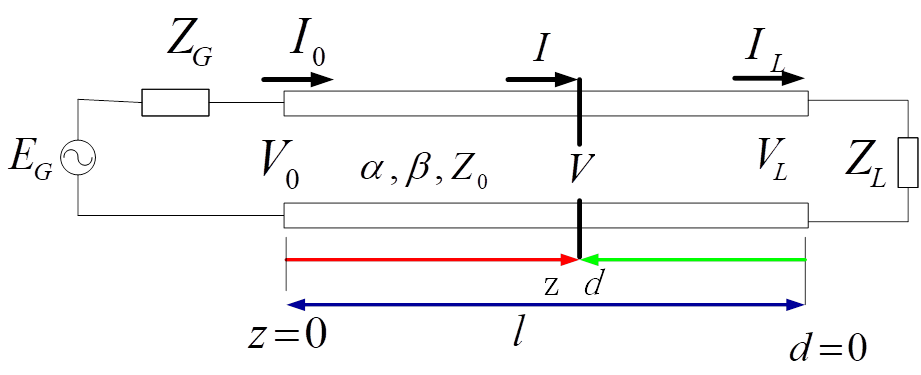
\includegraphics[width=8cm]{tmlineboundary.png}
 \begin{align*}
  \begin{bmatrix}
   V(d) \\I(d)
  \end{bmatrix}=
  \begin{bmatrix}
   \cosh\gamma d\quad Z_{0}\sinh\gamma d \\
   Z_{0}^{-1}\sinh\gamma d\quad \cosh\gamma d
  \end{bmatrix}
  \begin{bmatrix}
   V_{L} \\I_{L}
  \end{bmatrix}
 \end{align*}
 \flushleft
 传输线终端接负载阻抗$Z_{L}$时,距离终端$d$处向负载方向看去的输入阻抗定义为该处的电压$V(z)$与电流$I(z)$之比,即
\end{frame}

\begin{frame}{分布参数阻抗}
 \begin{empheq}[box=\widefbox]{align*}
  Z_{in}(d)=\frac{V_{L}\cosh\gamma d+I_{L}Z_{0}\sinh\gamma d}{I_{L}\cosh\gamma d+\frac{V_{L}\sin\beta d}{Z_{0}}}=Z_{0}\frac{Z_{L}+Z_{0}\tanh\gamma d}{Z_{0}+Z_{L}\tanh\gamma d}
 \end{empheq}
 \flushleft
 均匀无耗传输线\\
 $$\alpha=0,\gamma=j\beta,\tanh\gamma d=\tanh(j\beta d)=j\tan\beta d$$
 \begin{columns}
  \begin{column}{0.4\linewidth}
   传输线的阻抗(从$d$点向负载看的输入阻抗,或视在阻抗)
  \end{column}
  \begin{column}{0.6\linewidth}
   \begin{empheq}[box=\widefbox]{align*}
    Z_{in}(d)=Z_{0}\frac{Z_{L}+jZ_{0}\tan\beta d}{Z_{0}+jZ_{L}\tan\beta d}
   \end{empheq}
  \end{column}
 \end{columns}
 \flushleft
 对给定的传输线和负载阻抗,线上各点的输入阻抗随至终端的距离$d$的不同而作周期(周期为$\lambda/2$)变化,是一种\textbf{分布参数阻抗}。它不能直接测量。
\end{frame}

\begin{frame}{分布参数阻抗}
 \flushleft
 均匀无耗传输线\\
 \begin{empheq}[box=\widefbox]{align*}
  Z_{in}(d)=Z_{0}\frac{Z_{L}+jZ_{0}\tan\beta d}{Z_{0}+jZ_{L}\tan\beta d}
 \end{empheq}
 \begin{itemize}
  \item 传输线阻抗,随位置$d$而变,分布于沿线各点,且与负载有关,是一种分布参数阻抗(Distributed Impedance)。由于微波频率下,电压与电流缺乏明确的物理意义,不能直接测量,故传输线阻抗也不能直接测量。
  \item 传输线阻抗具有阻抗变换作用,$Z_{L}$通过线段$d$变换成$Z_{in}(d)$。
  \item 传输线阻抗呈现周期性变化。
 \end{itemize}
\end{frame}

\begin{frame}{分布参数阻抗}
 \flushleft
 在一些特殊位置点上,有如下简单阻抗关系:
 \begin{empheq}[box=\widefbox]{align*}
  & Z_{in}(l)=Z_{L}\qquad l=n\frac{\lambda}{2}(n=0,1,2,\ldots)\\
  & Z_{in}(l)=\frac{Z_{0}^{2}}{Z_{L}}\qquad l=(2n+1)\frac{\lambda}{4}(n=0,1,2,\ldots)
 \end{empheq}
 \begin{itemize}
  \item 传输线上距负载为半波长整数倍的各点输入阻抗等于负载阻抗;\textbf{半波长的重复性}
  \item 距负载为四分之一波长奇数倍的各点输入阻抗等于特性阻抗的平方与负载阻抗的比值
  \item 当$Z_{0}$为实数,$Z_{L}$为复数负载时,四分之一波长的传输线具有变换阻抗性质的作用。\textbf{四分之一波长变换性}
 \end{itemize}
\end{frame}

\begin{frame}
 \flushleft
 在许多情况下,例如并联电路的阻抗计算,采用导纳比较方便:
 \begin{empheq}[box=\widefbox]{align*}
  Y_{in}(d)=\frac{1}{Z_{in}(d)}=Y_{0}\frac{Y_{L}+jY_{0}\tan\beta d}{Y_{0}+jY_{L}\tan\beta d}
 \end{empheq}
\end{frame}

\begin{frame}{反射参量}
 \begin{enumerate}
  \resume
  \item 反射参量
        \saveenum
 \end{enumerate}
 \begin{empheq}[box=\widefbox]{align*}
  V(d)=\frac{V_{L}+I_{L}Z_{0}}{2}e^{\gamma d}+\frac{V_{L}-I_{L}Z_{0}}{2}e^{-\gamma d}
 \end{empheq}
 \begin{itemize}
  \item 反射系数(Reflection Coefficient)
 \end{itemize}
 距终端$d$处的反射波电压$V^{-}(d)$与入射波电压$V^{+}(d)$之比定义为该处的\textbf{电压反射系数}$\Gamma_{v}(d)$,即
 \begin{align*}
  \Gamma_{v}(d) & =\frac{V^{-}(d)}{V^{+}(d)}=\frac{A_{2}e^{-\gamma d}}{A_{1}e^{\gamma d}}                                \\
                & =\frac{V_{L}-I_{L}Z_{0}}{V_{L}+I_{L}Z_{0}}e^{-2\gamma d}=\frac{Z_{L}-Z_{0}}{Z_{L}+Z_{0}}e^{-2\gamma d}
 \end{align*}
\end{frame}

\begin{frame}{反射参量}
 \begin{columns}
  \begin{column}{0.35\linewidth}
   电流反射系数
  \end{column}
  \begin{column}{0.65\linewidth}
   \begin{empheq}[box=\widefbox]{align*}
    I(d)=\frac{V_{L}+I_{L}Z_{0}}{2Z_{0}}e^{\gamma d}-\frac{V_{L}-I_{L}Z_{0}}{2Z_{0}}e^{-\gamma d}
   \end{empheq}
  \end{column}
 \end{columns}
 \begin{align*}
  \Gamma_{I}(d)=\frac{I^{-}(d)}{I^{+}(d)}=-\frac{A_{2}}{A_{1}}e^{-2\gamma d}=-\Gamma_{V}(d)
 \end{align*}
 终端反射系数
 \begin{columns}
  \begin{column}{0.45\linewidth}
   \begin{align*}
     & \Gamma_{L}=\frac{A_{2}}{A_{1}}=\frac{Z_{L}-Z_{0}}{Z_{L}+Z_{0}}                                             \\
     & =\left\lvert\frac{Z_{L}-Z_{0}}{Z_{L}+Z_{0}}\right\rvert e^{j\Phi_{L}}=\lvert\Gamma_{L}\rvert e^{j\Phi_{L}}
   \end{align*}
  \end{column}
  \begin{column}{0.45\linewidth}
   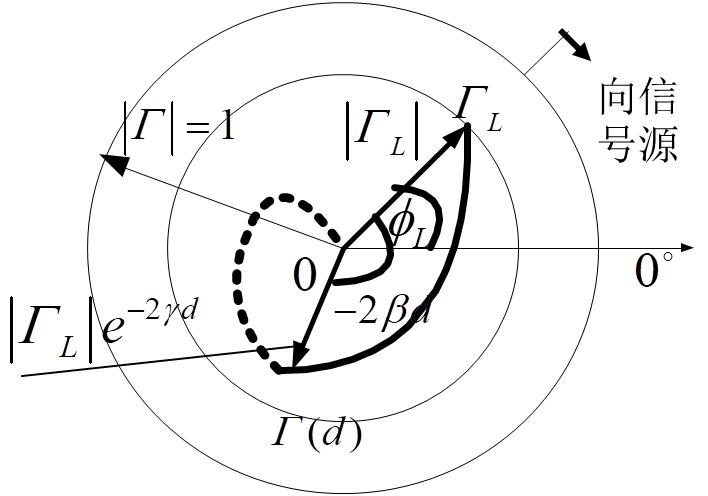
\includegraphics[width=4cm]{chart1.png}
  \end{column}
 \end{columns}
 $$\Gamma(d)=\Gamma_{L}e^{-2\gamma d}\text{传输线上任一点反射系数与终端反射系数的关系}$$
\end{frame}

\begin{frame}{反射参量}
 无耗线情况
 \begin{empheq}[box=\widefbox]{align*}
  \Gamma(d)=\Gamma_{L}e^{-j2\beta d}=\lvert\Gamma_{L}\rvert e^{j(\Phi_{L}-2\beta d)}
 \end{empheq}
 \begin{columns}
  \begin{column}{0.5\linewidth}
   $\Gamma(d)$的大小和相位均在单位圆内,大小不变,相位以$-2\beta d$的角度沿等圆周向信号源(顺时针)方向变化。
  \end{column}
  \begin{column}{0.5\linewidth}
   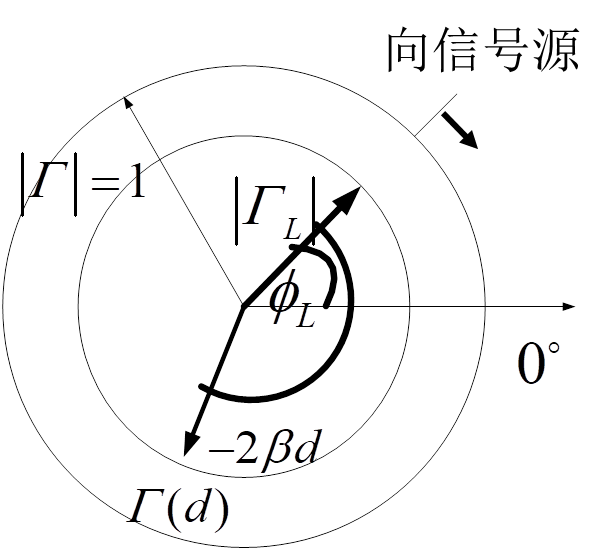
\includegraphics[width=4.5cm]{chart2.png}
  \end{column}
 \end{columns}
\end{frame}

\begin{frame}{反射参量}
 \begin{itemize}
  \item 阻抗与反射系数关系
 \end{itemize}
 \begin{align*}
   & V(d)=V^{+}(d)+V^{-}(d)=V^{+}(d)[1+\Gamma(d)] \\
   & I(d)=I^{+}(d)+I^{-}(d)=I^{+}(d)[1-\Gamma(d)]
 \end{align*}
 输入阻抗与反射系数间的关系
 \begin{empheq}[box=\widefbox]{align*}
  Z_{in}(d)=\frac{V^{+}(d)[1+\Gamma(d)]}{I^{+}(d)[1-\Gamma(d)]}=Z_{0}\frac{1+\Gamma(d)}{1-\Gamma(d)}
 \end{empheq}
\end{frame}

\begin{frame}{反射参量}
 \begin{empheq}[box=\widefbox]{align*}
  Z_{in}(d)=\frac{V^{+}(d)[1+\Gamma(d)]}{I^{+}(d)[1-\Gamma(d)]}=Z_{0}\frac{1+\Gamma(d)}{1-\Gamma(d)}
 \end{empheq}
 当传输线特性阻抗$Z_{0}$一定时,传输线上任意一点$d$处的阻抗$Z_{in}(d)$与该点的反射系数$\Gamma(d)$一一对应。可以通过测量反射系数获得传输线输入阻抗。\\
 \textbf{归一化}阻抗
 \begin{empheq}[box=\widefbox]{align*}
  z_{in}(d)=\frac{Z_{in}(d)}{Z_{0}}=\frac{1+\Gamma(d)}{1-\Gamma(d)}
 \end{empheq}
\end{frame}

\begin{frame}{反射参量}
 \begin{itemize}
  \item 传输系数$T$\qquad 描述传输线上的功率传输关系
 \end{itemize}
 \begin{columns}
  \begin{column}{0.5\linewidth}
   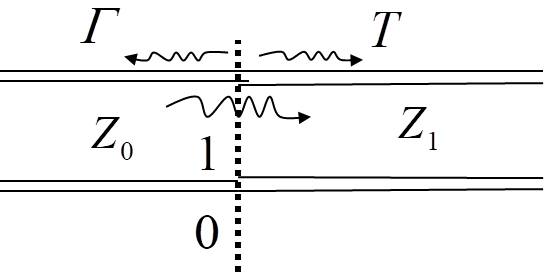
\includegraphics[width=4cm]{transPara.png}
  \end{column}
  \begin{column}{0.5\linewidth}
   \begin{align*}
    T=\frac{\text{传输电压或电流}}{\text{入射电压或电流}}=\frac{V^{t}}{V^{+}}=\frac{I^{t}}{I^{+}}
   \end{align*}
  \end{column}
 \end{columns}
 \begin{empheq}[box=\fbox]{align*}
  & V(z)=V^{+}_{0}(e^{-j\beta z}+\Gamma e^{j\beta z})\quad z<0\\
  & V(z)=V_{0}^{+}Te^{-j\beta z}\qquad\qquad\quad z>0
 \end{empheq}
 $Z=0$处两电压连续
 \begin{empheq}[box=\widefbox]{align*}
  T=1+\Gamma=1+\frac{Z_{1}-Z_{0}}{Z_{1}+Z_{0}}=\frac{2Z_{1}}{Z_{1}+Z_{0}}
 \end{empheq}
 插入损耗
 \begin{empheq}[box=\widefbox]{align*}
  L_{T}=-20\lg\lvert T \rvert \qquad (dB)
 \end{empheq}
\end{frame}

\begin{frame}{驻波参量}
 \begin{enumerate}
  \resume
  \item \textbf{驻波参量}
 \end{enumerate}
 \begin{itemize}
  \item 电压驻波比(VSWR)与行波系数K\\
        传输线上各点的电压和电流一般由入射波和反射波叠加而成,其结果在线上形成驻波,沿线各点的电压和电流的振幅不同,以$\lambda/2$周期变化。\\
        波腹点——振幅最大点\\
        波谷点——振幅最小点\qquad 波节点——振幅等于零的点\\
        \textbf{电压(或电流)驻波比VSWR}:定义为传输线上电压(或电流)振幅的最大值与最小值之比,或电压驻波系数$\rho$
        \begin{empheq}[box=\widefbox]{align*}
         VSWR=\rho=\frac{\lvert V\rvert_{max}}{\lvert V\rvert_{min}}=\frac{\lvert I\rvert_{max}}{\lvert I\rvert_{min}}
        \end{empheq}
 \end{itemize}
\end{frame}

\begin{frame}{驻波参量}
 \textbf{行波系数K}:定义为传输线上电压(或电流)的最小值与最大值之比,故行波系数与驻波比互为倒数。
 \begin{empheq}[box=\widefbox]{align*}
  K=\frac{1}{VSWR}=\frac{\lvert V\rvert_{min}}{\lvert V\rvert_{max}}=\frac{\lvert I\rvert_{min}}{\lvert I\rvert_{max}}
 \end{empheq}
\end{frame}

\begin{frame}{驻波参量}
 传输线任意点电压和电流
 \begin{align*}
  V(d)=V^{+}(d)[1+\lvert\Gamma_{L}\rvert e^{j(\Phi_{L}-2\beta d)}] \\
  I(d)=I^{+}(d)[1-\lvert\Gamma_{L}\rvert e^{j(\Phi_{L}-2\beta d)}]
 \end{align*}
 \begin{columns}
  \begin{column}{0.5\linewidth}
   当传输线上入射波与反射波同相叠加时,合成波出现最大值;而反向叠加时出现最小值。
  \end{column}
  \begin{column}{0.5\linewidth}
   \begin{align*}
    \lvert V(d)\rvert_{max}=v^{+}(d)[1+\lvert\Gamma_{L}\rvert] \\
    \lvert V(d)\rvert_{min}=v^{+}(d)[1-\lvert\Gamma_{L}\rvert]
   \end{align*}
  \end{column}
 \end{columns}
 驻波比与反射系数的关系式为:
 \begin{columns}
  \begin{column}{0.65\linewidth}
   \begin{empheq}[box=\widefbox]{align*}
    \rho=VSWR=\frac{\lvert V\rvert_{max}}{\lvert V\rvert_{min}}=\frac{1+\lvert\Gamma_{L}\rvert}{1-\lvert\Gamma_{L}\rvert}
   \end{empheq}
  \end{column}
  \begin{column}{0.35\linewidth}
   \begin{empheq}[box=\widefbox]{align*}
    \lvert\Gamma_{L}\rvert=\frac{\rho-1}{\rho+1}
   \end{empheq}
  \end{column}
 \end{columns}
\end{frame}

\begin{frame}{驻波参量}{沿线阻抗分布}
 线上任一点处的输入阻抗为:
 \begin{align*}
  Z_{in}(z)=Z_{0}\frac{Z_{L}+jZ_{0}\tan\beta z}{Z_{0}+jZ_{L}\tan\beta z}=R_{in}(z)+jX_{in}(z)
 \end{align*}
 (1)阻抗的数值周期性变化,在电压的波腹点和波谷点,阻抗分别为最大值和最小值
 \begin{align*}
  Z_{in}(波腹)=\frac{\lvert U\rvert_{max}}{\lvert I\rvert_{min}}=Z_{0}\frac{1+\lvert\Gamma\rvert}{1-\lvert\Gamma\rvert}=Z_{0}\rho\qquad \text{开路} \\
  Z_{in}(波谷)=\frac{\lvert U\rvert_{min}}{\lvert I\rvert_{max}}=Z_{0}\frac{1-\lvert\Gamma\rvert}{1+\lvert\Gamma\rvert}=Z_{0}\rho\qquad \text{短路}
 \end{align*}
 (2)每隔$\lambda/4$,阻抗性质变换一次;每隔$\lambda/2$,阻抗值重复一次。
\end{frame}

\begin{frame}{驻波参量}
 \begin{itemize}
  \item 阻抗与驻波参量的系数
 \end{itemize}
 由分布参数阻抗
 \begin{empheq}[box=\widefbox]{align*}
  Z_{in}(d)=Z_{0}\frac{Z_{L}+jZ_{0}\tan\beta d}{Z_{0}+jZ_{L}\tan\beta d}
 \end{empheq}
 \centering
 $\downarrow$
 \begin{empheq}[box=\widefbox]{align*}
  Z_{L}=Z_{0}\frac{Z_{in}(d)-jZ_{0}\tan\beta d}{Z_{0}-jZ_{in}(d)\tan\beta d}
 \end{empheq}
 \begin{columns}
  \begin{column}{0.6\linewidth}
   选取驻波最小点为测量点——距离负载的第一个电压驻波最小点位置
  \end{column}
  \begin{column}{0.4\linewidth}
   \begin{align*}
    Z_{in}(d_{min})=Z_{0}/VSWR=Z_{0}/\rho
   \end{align*}
  \end{column}
 \end{columns}
 \flushleft
 终端短路,确定电压波节点作参考点,接上负载测量参考点附近电压驻波最小点。
 \begin{columns}
  \begin{column}{0.5\linewidth}
   \begin{empheq}[box=\fbox]{align*}
    Z_{L}=Z_{0}\frac{1-j\rho\tan\beta d_{min}}{\rho-j\tan\beta d_{min}}
   \end{empheq}
  \end{column}
  \begin{column}{0.5\linewidth}
   负载阻抗和驻波参量一一对应
  \end{column}
 \end{columns}
\end{frame}

\subsection{无耗线工作状态分析}
\begin{frame}{无耗线工作状态}
 任何传输线上的电压函数只可能是入射波和反射波的迭加(构成Standing Wave)。不同传输线的区别仅仅在于入射波和反射波的成分不同。换句话说,通解是完备的,我们不需要再找,也不可能再找到其他解。\\
 边界条件确定$A_{1}$和$A_{2}$。边界条件的求取过程中,也孕育着一种思想,即网络思想(Network Idea):已知输入求输出;或已知输出求输入。
\end{frame}

\begin{frame}{无耗线工作状态}
 \begin{empheq}[box=\widefbox]{align*}
  V(z)=A_{1}e^{-j\beta z}+A_{2}e^{+j\beta z}
 \end{empheq}
 \begin{empheq}[box=\widefbox]{align*}
  V(d) & =\frac{1}{2}(V_{L}+Z_{0}I_{L})e^{j\beta d}+\frac{1}{2}(V_{L}-Z_{0}I_{L})e^{-j\beta d}\\
  & =V^{+}(d)+V^{-}(d)
 \end{empheq}
 \begin{empheq}[box=\widefbox]{align*}
  I(z)=\frac{1}{Z_{0}}(A_{1}e^{-j\beta z}+A_{2}e^{+j\beta z})
 \end{empheq}
 \begin{empheq}[box=\widefbox]{align*}
  I(d) & =\frac{1}{2Z_{0}}(V_{L}+Z_{0}I_{L})e^{j\beta d}-\frac{1}{2Z_{0}}(V_{L}-Z_{0}I_{L})e^{-j\beta d}\\
  & =I^{+}(d)+I^{-}(d)
 \end{empheq}
\end{frame}

\begin{frame}{无耗线工作状态}
 \begin{itemize}
  \item 传输线上反射波的大小,可用反射系数的模、驻波比和行波系数三个参量来描述。\\
        \begin{columns}
         \begin{column}{0.5\linewidth}
          反射系数模的变化范围为\\
          驻波比的变化范围为\\
          行波系数的变化范围为
         \end{column}
         \begin{column}{0.3\linewidth}
          \fbox{$0\leq\lvert\Gamma\rvert\leq 1$}\\
          \fbox{$1\leq\rho\leq\infty$}\\
          \fbox{$0\leq K\leq 1$}
         \end{column}
        \end{columns}
  \item 传输线的工作状态一般分为三种:\\
        (1)行波状态 \qquad $\lvert\Gamma\rvert=0,\rho=1,K=1$ \\
        (2)行驻波状态\quad $0<\lvert\Gamma\rvert<1 \quad 1<\rho<\infty \quad 0<K<1$\\
        (3)驻波状态 \qquad $\lvert\Gamma\rvert=1 \quad \rho=\infty \quad K=0$
 \end{itemize}
\end{frame}

\begin{frame}{无耗线工作状态}
 \begin{enumerate}
  \item \textbf{行波状态(无反射情况)}
        \begin{columns}
         \begin{column}{0.4\linewidth}
          条件:\\
          $Z_{L}=Z_{0}\rightarrow$\\
          $\Gamma_{L}=0,\rho=1,K=1$
         \end{column}
         \begin{column}{0.6\linewidth}
          \begin{empheq}[box=\widefbox]{align*}
           \Gamma_{L}=\frac{A_{2}}{A_{1}}=\frac{Z_{L}-Z_{0}}{Z_{L}+Z_{0}}\\
           =\left\lvert\frac{Z_{L}-Z_{0}}{Z_{L}+Z_{0}}\right\rvert e^{j\Phi_{L}}=\lvert\Gamma_{L}\rvert e^{j\Phi_{L}}
          \end{empheq}
         \end{column}
        \end{columns}
        由始端条件解
        \begin{empheq}[box=\widefbox]{align*}
         V(z)=\frac{V_{0}+I_{0}Z_{0}}{2}e^{-j\beta z}=V_{0}^{+}e^{-j\beta z}\\
         I(z)=\frac{V_{0}+I_{0}Z_{0}}{2Z_{0}}e^{-j\beta z}=I_{0}^{+}e^{-j\beta z}
        \end{empheq}
        \saveenum
 \end{enumerate}
\end{frame}

\begin{frame}{无耗线工作状态}
 \begin{columns}
  \begin{column}{0.5\linewidth}
   \begin{empheq}[box=\widefbox]{align*}
    v(z,t)=\lvert V_{0}^{+}\rvert\cos(\omega t-\phi_{0}-\beta z)\\
    i(z,t)=\lvert I_{0}^{+}\rvert\cos(\omega t-\phi_{0}-\beta z)
   \end{empheq}
   $\phi_{0}$为初相角,行波状态下的分布规律:\\
   (1)线上电压和电流的振幅恒定不变\\
   (2)电压行波与电流行波同相,它们的相位是位置$z$和时间$t$的函数,$v(z,t)$和$i(z,t)$初相均为$\phi_{0}$,因为$Z_{0}$是实数\\
   (3)线上的输入阻抗处处相等,且均等于特性阻抗
  \end{column}
  \begin{column}{0.5\linewidth}
   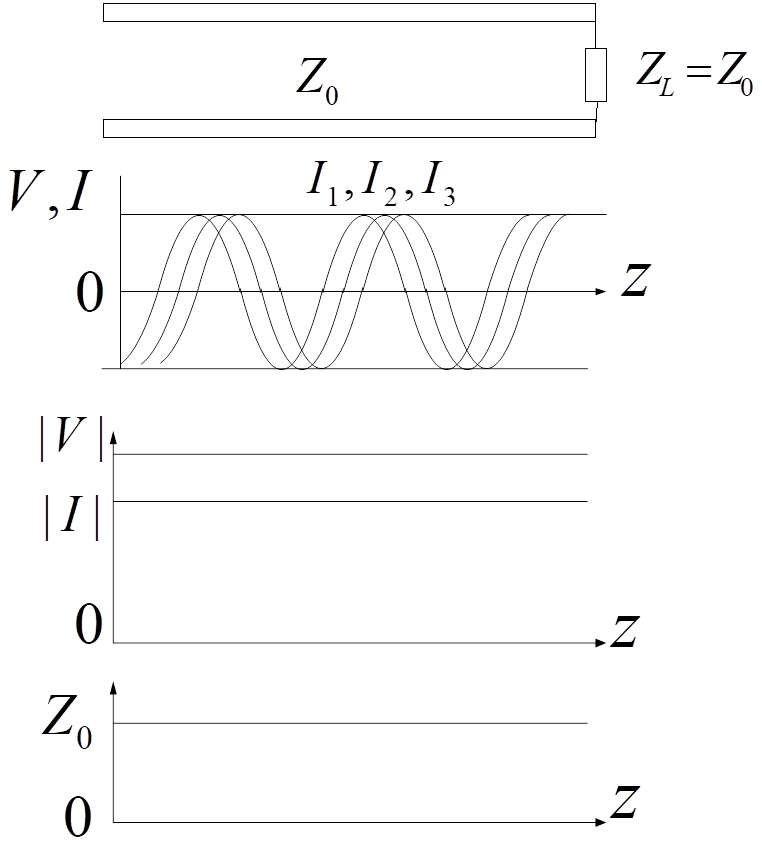
\includegraphics[width=5cm]{xingbo.png}
  \end{column}
 \end{columns}
\end{frame}

\begin{frame}{无耗线工作状态}
 \begin{enumerate}
  \resume
  \item \textbf{驻波状态(全反射情况)}
        \saveenum
 \end{enumerate}
 反射系数模等于1的全反射情况称为驻波状态。
 \begin{empheq}[box=\widefbox]{align*}
  \Gamma_{L}=\frac{A_{2}}{A_{1}}=\frac{Z_{L}-Z_{0}}{Z_{L}+Z_{0}}=\left\lvert\frac{Z_{L}-Z_{0}}{Z_{L}+Z_{0}}\right\rvert e^{j\phi_{L}}=\lvert\Gamma_{L}\rvert e^{j\phi_{L}}
 \end{empheq}
 条件:终端短路;终端开路;终端接纯电抗负载\\
 \qquad \quad$Z_{L}=0$,\qquad$Z_{L}=\infty$,\qquad$Z_{L}=\pm jX_{L}$\\
 终端的入射波将被全反射,沿线入射波与反射波迭加形成驻波分布。驻波状态意味着入射波功率一点也没有被负载吸收,即\textbf{负载与传输线完全失配}。
\end{frame}

\begin{frame}{无耗线工作状态}
 \begin{itemize}
  \item 终端短路
 \end{itemize}
 \begin{empheq}[box=\widefbox]{align*}
  Z_{L}=0,\Gamma_{L}=\frac{Z_{L}-Z_{0}}{Z_{L}+Z_{0}}=-1\rightarrow VSWR=\frac{1+\lvert\Gamma_{L}\rvert}{1-\lvert\Gamma_{L}\rvert}=\infty
 \end{empheq}
 \begin{align*}
  V(d) & =V^{+}(d)+V^{-}(d)=V_{L}^{+}(e^{j\beta d}-e^{-j\beta d})=j2V_{L}^{+}\sin\beta d \\
  I(d) & =I^{+}(d)+I^{-}(d)=I_{L}^{+}(e^{j\beta d}+e^{-j\beta d})=2I_{L}^{+}\cos\beta d  \\
       & =\frac{2V_{L}^{+}}{Z_{0}}\cos\beta d
 \end{align*}
 短路时的驻波状态分布规律:\\
 (1)瞬时电压或电流在传输线的某个固定位置上随时间$t$作正弦或余弦变化,而在某一时刻随位置$d(z)$也作正弦或余弦变化,但瞬时电压和电流的时间相位差和空间相位差均为$\pi/2$,这表明传输线上没有功率传输。
\end{frame}

\begin{frame}{无耗线工作状态}
 \only<1>{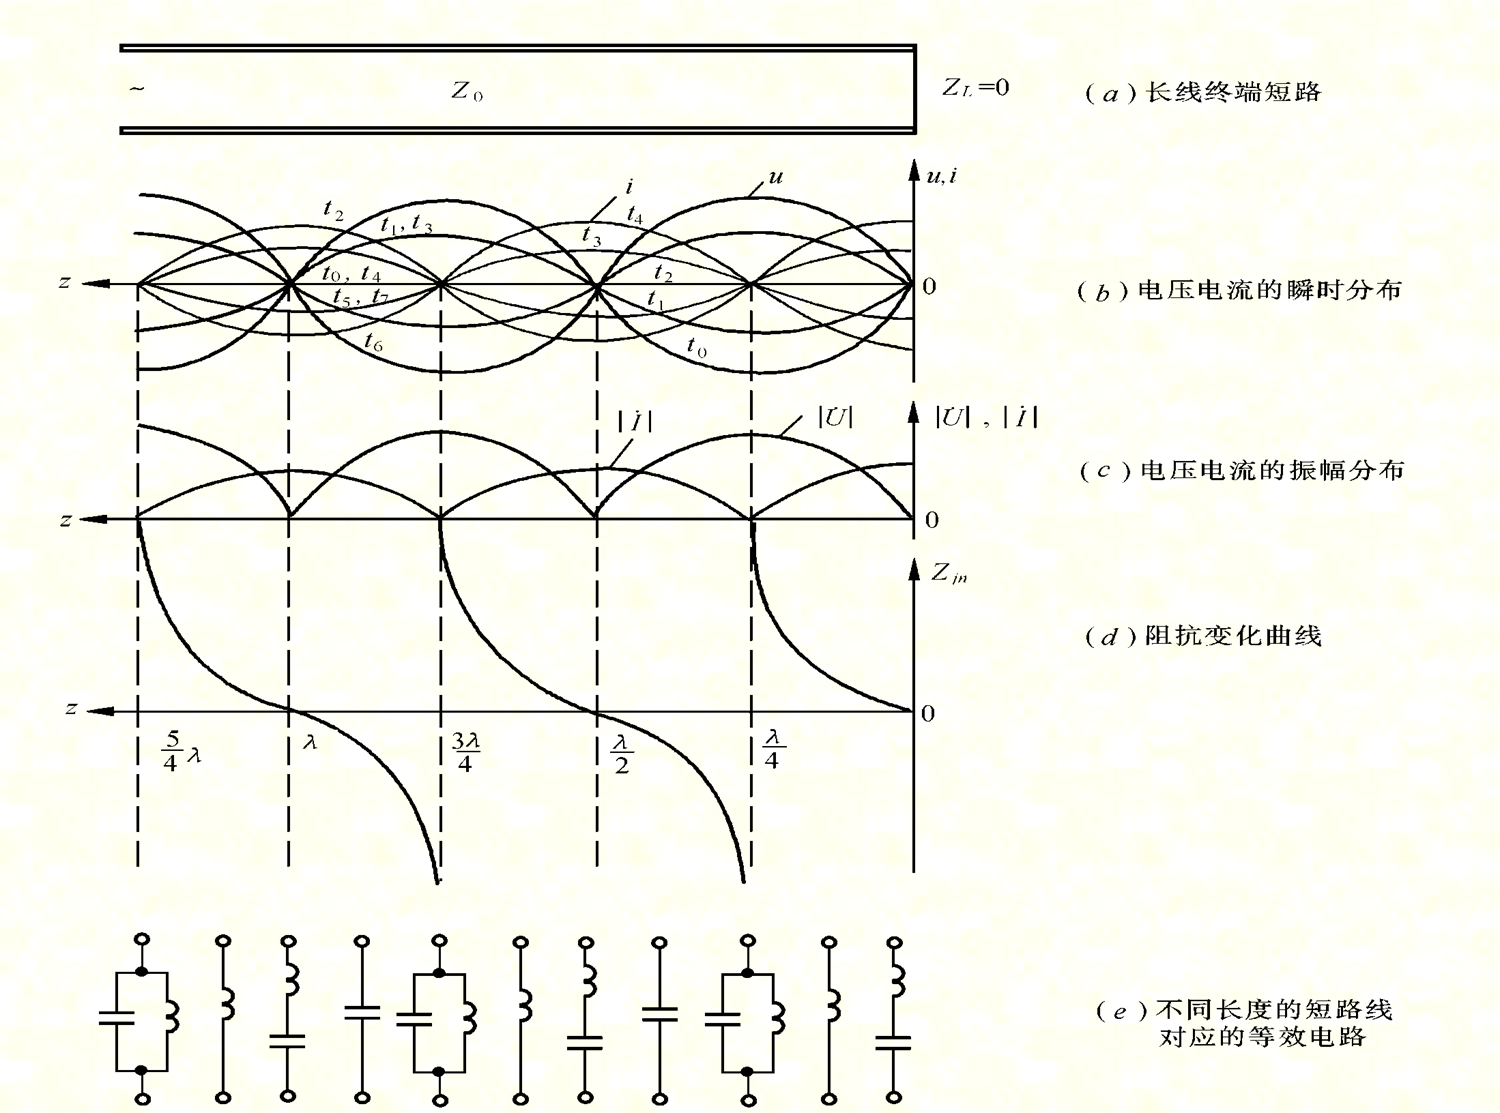
\includegraphics[width=10cm]{duanlu.png}}
 \only<2>{\begin{columns}
   \begin{column}{0.55\linewidth}
    \begin{empheq}[box=\widefbox]{align*}
     d=(2n+1)\lambda/4,(n=0,1,\ldots)\\
     \lvert V\rvert_{max}=2\lvert V_{L}^{+}\rvert
    \end{empheq}
    \begin{empheq}[box=\widefbox]{align*}
     d=n\lambda/2,(n=0,1,\ldots)\\
     \lvert V\rvert_{min}=0
    \end{empheq}
   \end{column}
   \begin{column}{0.45\linewidth}
    (2)电压振幅最大值,而电流振幅恒为零,这些点称之为电压的波腹点和电流的波节点;\\
    电流振幅恒为最大值,而电压振幅恒为零,这些点称之为电流的波腹点和电压的波节点。
   \end{column}
  \end{columns}}
 \only<3>{
  \begin{table}[h!]
   \begin{center}
    \caption{终端短路情况}
    \begin{tabular}{|c|c|}
     \hline
     $ \beta d=n\pi $                                           & $ \beta d=(2n+1)\pi/2 $                                    \\
     $ d=n\lambda/2 $                                           & $ d=(2n+1)\lambda/4 $                                      \\
     \hline
     $\text{电压节点}\lvert V(d)\rvert=0$                       & $\text{电压腹点}\lvert V(d)\rvert=2\lvert V_{L}^{+}\rvert$ \\
     $\text{电流腹点}\lvert I(d)\rvert=2\lvert I_{L}^{+}\rvert$ & $ \text{电流节点}\lvert I(d)\rvert=0$                      \\
     \hline
    \end{tabular}
   \end{center}
  \end{table}
 }
 \only<4>{(3)传输线终端短路时,输入阻抗为纯电抗。\\
  \begin{empheq}[box=\widefbox]{align*}
   Z_{in}^{sc}(d)=Z_{0}\frac{Z_{L}+jZ_{0}\tan\beta d}{Z_{0}+jZ_{L}\tan\beta d}=jZ_{0}\tan\beta d=jZ_{0}\tan\frac{2\pi d}{\lambda}=jX_{in}
  \end{empheq}}
\end{frame}

\begin{frame}{无耗线工作状态}
 \begin{itemize}
  \item 终端开路
 \end{itemize}
 \begin{empheq}[box=\widefbox]{align*}
  Z_{L}=\infty,\Gamma_{L}=\frac{Z_{L}-Z_{0}}{Z_{L}+Z_{0}}=1\rightarrow VSWR=\frac{1+\lvert\Gamma_{L}\rvert}{1-\lvert\Gamma_{L}\rvert}=\infty
 \end{empheq}
 \begin{align*}
   & \Gamma_{L}=V_{L}^{-}/V_{L}^{+}=1 \quad V_{L}^{-}=V_{L}^{+} \\
   & V(d)=V^{+}(d)+V^{-}(d)=2V_{L}^{+}\cos\beta d               \\
   & I(d)=I^{+}(d)+I^{-}(d)=j2I_{L}^{+}\sin\beta d              \\
   & Z_{in}^{oc}(d)=-jZ_{0}\cot\beta d
 \end{align*}
 \begin{columns}
  \begin{column}{0.5\linewidth}
   终端短路
   \begin{empheq}[box=\widefbox]{align*}
    Z_{L}=0,\Gamma_{L}=-1\rightarrow VSWR=\infty
   \end{empheq}
  \end{column}
  \begin{column}{0.5\linewidth}
   \begin{empheq}[box=\widefbox]{align*}
    & V(d)=j2V_{L}^{+}\sin\beta d\\
    & I(d)=2I_{L}^{+}\cos\beta d\\
    & Z_{in}^{sc}(d)=jZ_{0}\tan\beta d
   \end{empheq}
  \end{column}
 \end{columns}
\end{frame}

\begin{frame}{无耗线工作状态}
 (1)负载处,或\fbox{$d=n\lambda/2,(n=0,1,\ldots)$}\\
 电流$I_{L}=0$为电流波节点,\\
 电压为最大值$V_{L}=2V_{L}^{+}$为电压波腹点
 \begin{table}[h!]
  \begin{center}
   \caption{终端开路情况}
   \begin{tabular}{|c|c|}
    \hline
    $\beta d=n\pi$                                      & $\beta d=(2n+1)\pi/2$                               \\
    $d=n\lambda/2$                                      & $d=(2n+1)\lambda/4$                                 \\
    \hline
    电压腹点$\lvert V(d)\rvert=2\lvert V_{L}^{+}\rvert$ & 电压节点$\lvert V(d)=0\rvert$                       \\
    电流节点$\lvert I(d)=0\rvert$                       & 电流腹点$\lvert I(d)\rvert=2\lvert I_{L}^{+}\rvert$ \\
    \hline
   \end{tabular}
  \end{center}
 \end{table}
 (2)输入阻抗\\
 $Z_{in}^{oc}(d)=-jZ_{0}\cot\beta d\Longleftrightarrow$ 短路 \fbox{$Z_{in}^{sc}=jZ_{0}\tan\beta d$}\\
 经过观察:\textbf{把开路线可以看成是短路线移动$\lambda/4$而成}
\end{frame}

\begin{frame}{无耗线工作状态}
 \begin{columns}
  \begin{column}{0.5\linewidth}
   短路状态
   \begin{empheq}[box=\widefbox]{align*}
    & V(d)=j2V_{L}^{+}\sin\beta d\\
    & I(d)=2I_{L}^{+}\cos\beta d
   \end{empheq}
   \begin{empheq}[box=\widefbox]{align*}
    Z(d)=jZ_{0}\tan\beta d
   \end{empheq}
   作$d'=d+\lambda/4,V_{L}^{+}=j\tilde V_{L}^{+}$变换,即可由开路线转化为短路线。不能疏忽了$V_{L}^{+}=j\tilde V_{L}^{+}$的条件,长度$d'$移动条件只对$\lvert V_{L}^{+}\rvert$和阻抗有效,\textbf{相位}是不等价的。
  \end{column}
  \begin{column}{0.5\linewidth}
   开路状态
   \begin{empheq}[box=\widefbox]{align*}
    & V(d)=2V_{L}^{+}\cos\beta d\\
    & I(d)=j2I_{L}^{+}\sin\beta d
   \end{empheq}
   \centering
   $\Downarrow$
   \begin{empheq}[box=\widefbox]{align*}
    & V(d')=j2\tilde V_{L}^{+}\sin\beta d'\\
    & I(d')=2\tilde I_{L}^{+}\cos\beta d'
   \end{empheq}
   \begin{empheq}[box=\widefbox]{align*}
    Z(d)=-jZ_{0}\cot\beta d
   \end{empheq}
   $\Downarrow$
   \begin{empheq}[box=\widefbox]{align*}
    Z(d')=jZ_{0}\tan\beta d'
   \end{empheq}
  \end{column}
 \end{columns}
\end{frame}

\begin{frame}{无耗线工作状态}
 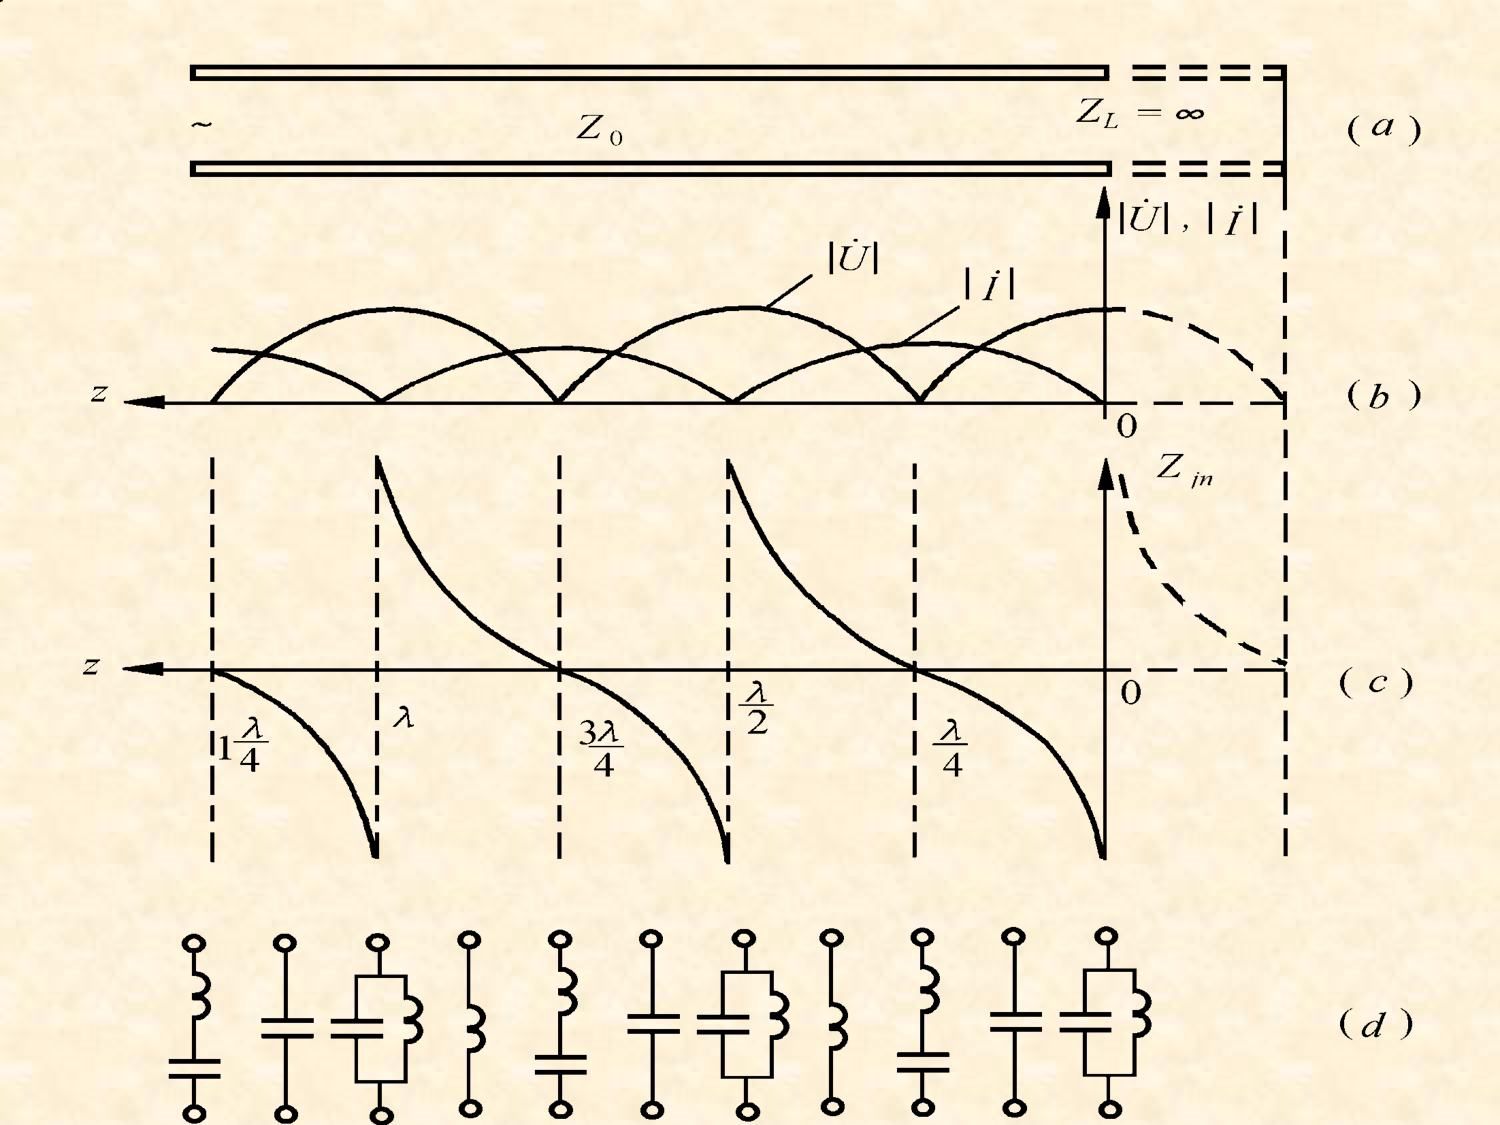
\includegraphics[width=10cm]{kailu.png}
\end{frame}

\begin{frame}{无耗线工作状态}
 \begin{align*}
  Z_{in}^{oc}(d)=-jZ_{0}\cot\beta d \qquad Z_{in}^{sc}(d)=jZ_{0}\tan\beta d \\
  Z_{in}^{oc}(d)\cdot Z_{in}^{sc}(d)=Z_{0}^{2}
 \end{align*}
 \begin{itemize}
  \item 对于一定长度$d$的传输线,通过开路和短路的测量,可以得到如下参数:
 \end{itemize}
 \begin{align*}
   & Z_{0}=\sqrt{Z_{in}^{oc}(d)\cdot Z_{in}^{sc}(d)}                      \\
   & \beta=\frac{1}{d}\arctan\sqrt{\frac{Z_{in}^{sc}(d)}{Z_{in}^{oc}(d)}}
 \end{align*}
\end{frame}

\begin{frame}{无耗线工作状态}
 \begin{itemize}
  \item 终端接\textbf{纯电感}负载无耗线\quad \fbox{$Z_{L}=+jX_{L}$}
 \end{itemize}
 \begin{align*}
  \Gamma_{L} & =\frac{Z_{L}-Z_{0}}{Z_{L}+Z_{0}}=\frac{jX_{L}-Z_{0}}{jX_{L}+Z_{0}}=\frac{(jX_{L}-Z_{0})^2}{(jX_{L}+Z_{0})(jX_{L}-Z_{0})} \\
             & =\frac{Z_{0}^{2}-X_{L}^{2}-2jZ_{0}X_{L}}{Z_{0}^{2}+X_{L}^{2}}=\lvert\Gamma_{L}\rvert e^{j\phi_{L}}
 \end{align*}
 \begin{align*}
  \therefore\lvert\Gamma_{L}\rvert=\frac{\sqrt{(Z_{0}^{2}-X_{L}^{2})^2+4Z_{0}^{2}X_{L}^{2}}}{Z_{0}^{2}+X_{L}^{2}}=\frac{\sqrt{(Z_{0}^{2}+X_{L}^{2})^2}}{Z_{0}^{2}+X_{L}^{2}}=1
 \end{align*}
 \begin{empheq}[box=\widefbox]{align*}
  \phi_{L}=\arctan\frac{2X_LZ_0}{X_L^2-Z_0^2}
 \end{empheq}
 终端产生全反射,形成驻波,但终端既不是电压波腹点也不是波节点
\end{frame}

\begin{frame}{无耗线工作状态}
 \begin{columns}
  \begin{column}{0.55\linewidth}
   可见此时终端也产生全反射,线上形成驻波;但此时终端$(d=0)$既不是电压波节点也不是电压波腹点。沿线的电压、电流和阻抗分布曲线可将电感负载用一段小于$\lambda/4$的短路线来等效后获得。
  \end{column}
  \begin{column}{0.45\linewidth}
   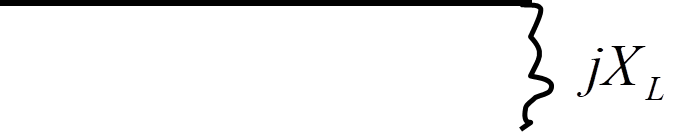
\includegraphics[width=4.5cm]{diangan1.png}
   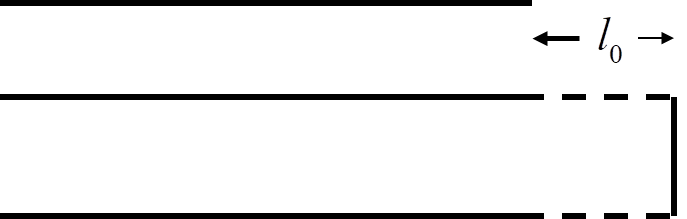
\includegraphics[width=4.5cm]{diangan2.png}
  \end{column}
 \end{columns}
 \begin{columns}
  \begin{column}{0.55\linewidth}
   短路线输入阻抗:
   \begin{empheq}[box=\widefbox]{align*}
    Z_{in}^{sc}(d)=jZ_{0}\tan\beta d=jX_{L}
   \end{empheq}
   故有等效短路线长度:
   \begin{empheq}[box=\widefbox]{align*}
    l_{es}& =\frac{1}{\beta}\tan^{-1}\left(\frac{X_L}{Z_0}\right)\\
    & =\frac{\lambda}{2\pi}\arctan\left(\frac{X_L}{Z_0}\right)
   \end{empheq}
  \end{column}
  \begin{column}{0.45\linewidth}
   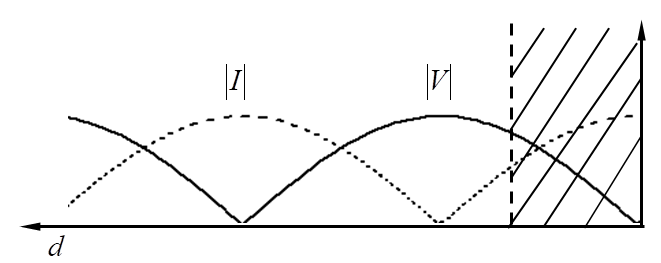
\includegraphics[width=4.5cm]{diangan3.png}
   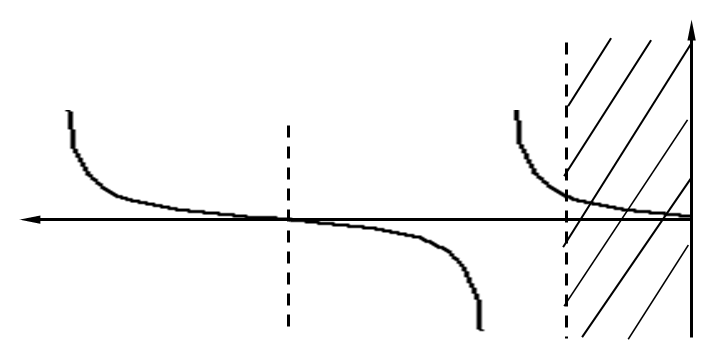
\includegraphics[width=4.5cm]{diangan4.png}
  \end{column}
 \end{columns}
\end{frame}

\begin{frame}{无耗线工作状态}
 \begin{itemize}
  \item 终端接\textbf{纯电容}负载无耗线\quad \fbox{$Z_L=-jX_L$}
 \end{itemize}
 \begin{align*}
  \Gamma_L=\frac{Z_L-Z_0}{Z_L+Z_0}=\frac{jX_L+Z_0}{jX_L-Z_0}=\lvert\Gamma_L\rvert e^{-j\phi_L} \\
  \lvert\Gamma_L\rvert=1 \qquad \phi_L=\arctan\frac{-2X_{L}Z_{0}}{X_{L}^{2}-Z_{0}^{2}}
 \end{align*}
 可见此时终端也产生全反射,线上形成驻波;但此时终端$(d=0)$既不是电压波节点也不是电压波腹点。沿线的电压、电流和阻抗分布曲线可将电容负载用一段小于$\lambda/4$的开路线来等效后获得。
 \begin{align*}
  Z_{in}^{oc}(d)=-jZ_0\cot\beta d=-jX_L
 \end{align*}
 \begin{empheq}[box=\widefbox]{align*}
  l_{eo} =\frac{1}{\beta}\cot^{-1}\left(\frac{X_L}{Z_0}\right)=\frac{\lambda}{2\pi}\cot^{-1}\left(\frac{X_L}{Z_0}\right)
 \end{empheq}
\end{frame}

\begin{frame}{无耗线工作状态}
 \centering
 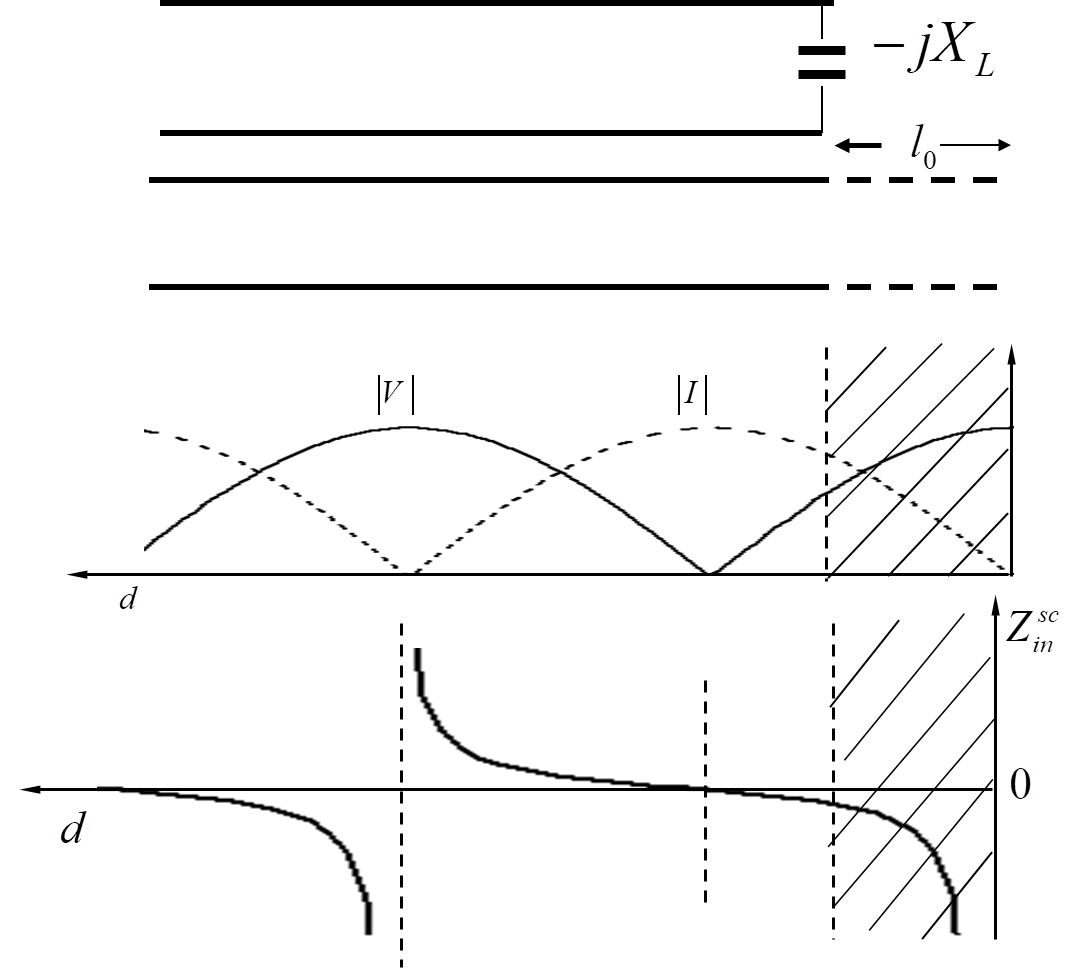
\includegraphics[width=8.5cm]{dianrong.png}
\end{frame}

\begin{frame}{无耗线工作状态}
 阻抗的一般公式\quad \fbox{$Z_L=jX_L$}
 \begin{align*}
  Z_{in}(d) & =Z_{0}\frac{Z_L+jZ_0\tan\beta d}{Z_0+jZ_L\tan\beta d}                                                                   \\
            & =jZ_0\frac{X_L+Z_0\tan\beta d}{Z_0-X_L\tan\beta d}=jZ_0\frac{\frac{X_L}{Z_0}+\tan\beta d}{1-\frac{X_L}{Z_0}\tan\beta d}
 \end{align*}
 此电抗也可用一段特性阻抗为$Z_0$、长度为$l_0$的短路线等效,长度$l_0$可由下式确定\\
 假设:$$\frac{X_L}{Z_0}=\tan\beta l_0 \qquad Z_{in}(d)=jZ_0\tan\beta(d+l_0)$$
 \begin{align*}
  l_0=\frac{\lambda}{2\pi}\arctan\frac{X_L}{Z_0}\quad \Longrightarrow \quad
  \left\{
  \begin{aligned}
   l_0>0 \quad X_L\text{为感性} \\
   l_0<0 \quad X_L\text{为容性}
  \end{aligned}
  \right.
 \end{align*}
\end{frame}

\begin{frame}{无耗线工作状态}
 \begin{empheq}[box=\widefbox]{align*}
  X_L=Z_0\tan\frac{2\pi}{\lambda}l_0\quad \Longrightarrow \quad l_0=\frac{\lambda}{2\pi}\arctan\frac{X_L}{Z_0}
 \end{empheq}
 长度为$l$终端接电抗性负载的传输线,沿线电压、电流及阻抗的变化规律与\textbf{长度为$(l+l_0)$的短路线}上对应段的变化规律完全一致,距终端最近的电压波节点
 \begin{align*}
  \left\{
  \begin{aligned}
   0<d<\lambda/4 \qquad \text{纯感抗} \\
   \lambda/4<d<\lambda/2 \qquad \text{纯容抗}
  \end{aligned}
  \right.
 \end{align*}
\end{frame}

\begin{frame}{无耗线工作状态}
 \centering
 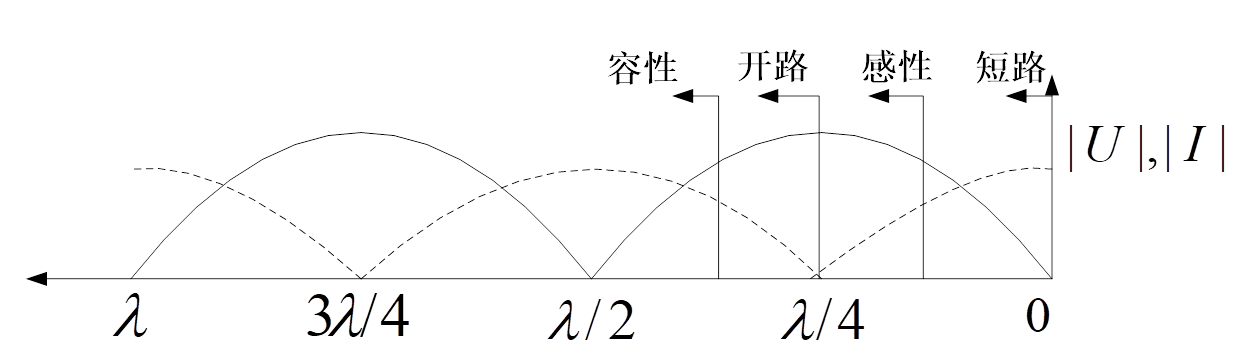
\includegraphics[width=8cm]{LandC.png}\\
 \flushleft
 综上所述,均匀无耗传输线终端无论是短路、开路还是接纯电抗负载,终端均产生全反射,沿线电压电流呈驻波分布,只是终端不同。\\
 1、\textbf{短路}:电压按正弦变化,电流按余弦变化,终端电压为零,电流为最大;\\
 \textbf{开路}:电压按余弦变化,电流按正弦变化,终端电流为零,电压为最大;\\
 \textbf{纯电抗}:电压、电流按正余弦变化,终端电压和电流不为零,也不是最大。
\end{frame}

\begin{frame}{无耗线工作状态}
 2、二分之一波长的重复性,四分之一波长的变化性。\\
 3、驻波波腹值为入射波的两倍,波节值等于零。短路线终端为电压波节、电流波腹;开路线终端为电压波腹、电流波节;接纯电抗负载时,终端既非波腹也非波节(\textbf{纯电感负载时,距负载第一个出现的是电压波腹点})。\\
 4、沿线同一位置的电压电流之间$90^\circ$相位差,所以驻波状态只有能量的存贮并无能量的传输。
\end{frame}

\begin{frame}{无耗线工作状态}
 \begin{enumerate}
  \resume
  \item \textbf{行驻波状态(部分反射情况)}\quad \fbox{$Z_L=R_L\pm jX_L$}
 \end{enumerate}
 条件:当均匀无耗传输线终端接一般复阻抗,产生部分反射,在线上形成行驻波。
 \begin{empheq}[box=\widefbox]{align*}
  \Gamma_L & =\frac{Z_L-Z_0}{Z_L+Z_0}=\frac{(R_L\pm jX_L)-Z_0}{(R_L\pm jX_L)+Z_0}\\
  & = \frac{R_L^2-Z_0^2+X_L^2}{(R_L+Z_0)^2+X_L^2}\pm j\frac{2X_LZ_0}{(R_L+Z_0)^2+X_L^2}\\
  & = \Gamma_{L1}\pm j\Gamma_{L2}=\lvert \Gamma_L\rvert e^{\pm j\phi_L}
 \end{empheq}
\end{frame}

\begin{frame}{无耗线工作状态}
 \widefbox{$\Gamma_L=\lvert\Gamma_L\rvert e^{\pm j\phi_L}$}
 \begin{align*}
   & \lvert\Gamma_L\rvert=\sqrt{\frac{(R_L-Z_0)^2+X_L^2}{(R_L+Z_0)^2+X_L^2}}<1 \\
   & \phi_L=\arctan\frac{\pm 2X_LZ_0}{R_L^2+X_L^2-Z_0^2}
 \end{align*}
 传输线工作在行驻波状态,行波与驻波的相对大小决定于负载与传输线的失配程度。
\end{frame}

\begin{frame}{无耗线工作状态}
 1、沿线电压、电流分布\\
 从
 \begin{align*}
  V(d)=V^+(d)[1+\lvert\Gamma_L\rvert e^{j(\phi_L-2\beta d)}] \\
  I(d)=I^+(d)[1-\lvert\Gamma_L\rvert e^{j(\phi_L-2\beta d)}]
 \end{align*}
 \begin{empheq}[box=\widefbox]{align*}
  V(d)=V_L^+e^{j\beta d}[1+\lvert\Gamma_L\rvert e^{\phi_L-2\beta d}]\\
  I(d)=I_L^+e^{j\beta d}[1-\lvert\Gamma_L\rvert e^{\phi_L-2\beta d}]
 \end{empheq}
 $\xLongrightarrow{\text{取模}}$
 \begin{align*}
   & \lvert V\rvert_{max}=V_L^+[1+\lvert\Gamma_L\rvert] \qquad \lvert V\rvert_{min}=V_L^+[1-\lvert\Gamma_L\rvert]      \\
   & \lvert I\rvert_{max}=I_L^+[1+\lvert\Gamma_L\rvert] \qquad\quad \lvert I\rvert_{min}=I_L^+[1-\lvert\Gamma_L\rvert]
 \end{align*}
 此时$\lvert\Gamma\rvert<1$,终端产生部分反射,线上形成行驻波,无波节点,驻波最小值不等于零,驻波最大值不等于终端入射波振幅的两倍。
\end{frame}

\begin{frame}{无耗线工作状态}
 \begin{align*}
  \lvert V(d)\rvert=\lvert V^+(d)\rvert[1+\lvert\Gamma_L\rvert^2+2\lvert\Gamma_L\rvert\cos(\phi_L-2\beta d)]^{1/2} \\
  \lvert I(d)\rvert=\lvert I^+(d)\rvert[1+\lvert\Gamma_L\rvert^2-2\lvert\Gamma_L\rvert\cos(\phi_L-2\beta d)]^{1/2}
 \end{align*}
 当$\cos(\phi_L-2\beta d)=1$\quad $\Longrightarrow$\quad \widefbox{$\phi_L-2\beta d=-2n\pi$}\\
 电压驻波最大点位置
 \begin{empheq}[box=\widefbox]{align*}
  d_{max}=\frac{\lambda}{4\pi}\phi_L+n\frac{\lambda}{2}\quad n=0,1,2,\ldots
 \end{empheq}
 当$\cos(\phi_L-2\beta d)=-1$\quad $\Longrightarrow$\quad \widefbox{$\phi_L-2\beta d=-\pi-2n\pi$}\\
 电压驻波最小点位置
 \begin{empheq}[box=\widefbox]{align*}
  d_{min}=\frac{\lambda}{4\pi}\phi_L+\frac{\lambda}{4}(2n+1)\quad n=0,1,2,\ldots
 \end{empheq}
\end{frame}

\begin{frame}{无耗线工作状态}
 2、阻抗分布
 \begin{align*}
  Z_{in}(d)  =Z_0\frac{1+\lvert\Gamma_L\rvert e^{-j(2\beta d-\phi_L)}}{1-\lvert\Gamma_L\rvert e^{-j(2\beta d-\phi_L)}}=Z_0\frac{e^{j(\beta d-\frac{1}{2}\phi_L)}+\lvert\Gamma_L\rvert e^{-j(\beta d-\frac{1}{2}\phi_L)}}{e^{j(\beta d-\frac{1}{2}\phi_L)}-\lvert\Gamma_L\rvert e^{-j(\beta d-\frac{1}{2}\phi_L)}} \\
  = Z_0\frac{(1+\lvert\Gamma_L\rvert)\cos\left(\beta d-\frac{1}{2}\phi_L\right)+j(1-\lvert\Gamma_L\rvert)\sin\left(\beta d-\frac{1}{2}\phi_L\right)}{(1-\lvert\Gamma_L\rvert)\cos\left(\beta d-\frac{1}{2}\phi_L\right)+j(1+\lvert\Gamma_L\rvert)\sin\left(\beta d-\frac{1}{2}\phi_L\right)}
 \end{align*}
 \begin{empheq}[box=\widefbox]{align*}
  Z_{in}(d)=Z_0\frac{\left(\frac{1+\lvert\Gamma_L\rvert}{1-\lvert\Gamma_L\rvert}\right)+j\tan\left(\beta d-\frac{1}{2}\phi_L\right)}{1+j\left(\frac{1+\lvert\Gamma_L\rvert}{1-\lvert\Gamma_L\rvert}\right)\tan\left(\beta d-\frac{1}{2}\phi_L\right)}
 \end{empheq}
 \begin{empheq}[box=\widefbox]{align*}
  \rho=\frac{1+\lvert\Gamma_L\rvert}{1-\lvert\Gamma_L\rvert}
 \end{empheq}
\end{frame}

\begin{frame}{无耗线工作状态}
 \begin{align*}
   & \cos(\phi_L-2\beta d)=1,\qquad \text{(V最大 I最小)} \\
   & Z_{in}=R_{max}+jX_{max}=Z_0\rho                     \\
   & R_{max}=Z_0\rho;X_{max}=0
 \end{align*}
 \hspace*{\fill}
 \begin{align*}
   & \cos(\phi_L-2\beta d)=-1,\qquad \text{(V最小 I最大)} \\
   & Z_{in}=R_{min}+jX_{min}=Z_0/\rho                     \\
   & R_{min}=Z_0/\rho=Z_0K;X_{min}=0
 \end{align*}
 \hspace*{\fill}
 \begin{align*}
   & \text{电压最大、最小点阻抗均为实数,二者相距}\lambda/4, \\
   & R_{max}R_{min}=Z_{0}^{2}
 \end{align*}
\end{frame}

\subsection{有耗线的特性与计算}
\begin{frame}{有耗线的特性与计算}

\end{frame}

\subsection{Smith Chart(阻抗圆图及其应用)}
\begin{frame}{Smith Chart(阻抗圆图及其应用)}
 前面的分析都是围绕如下公式及相互关系展开的:
 \begin{empheq}[box=\widefbox]{align*}
  Z_{in}(d)=\frac{V_L\cosh\gamma d+I_LZ_0\sinh\gamma d}{I_L\cosh\gamma d+\frac{V_L\sinh\gamma d}{Z_0}} & =Z_0\frac{Z_L+Z_0\tanh\gamma d}{Z_0+Z_L\tanh\gamma d}\\
  \text{无耗传输线:}& =Z_0\frac{Z_L+jZ_0\tan\beta d}{Z_0+jZ_L\tan\beta d}
 \end{empheq}
 \begin{columns}
  \begin{column}{0.45\linewidth}
   \begin{empheq}[box=\widefbox]{align*}
    \Gamma_L &=\frac{A_2}{A_1}=\frac{Z_L-Z_0}{Z_L+Z_0}\\
    &=\left\lvert\frac{Z_L-Z_0}{Z_L+Z_0}\right\rvert e^{j\phi_L}\\
    &=\lvert\Gamma_L\rvert e^{j\phi_L}
   \end{empheq}
  \end{column}
  \begin{column}{0.55\linewidth}
   \begin{empheq}[box=\widefbox]{align*}
    \rho=VSWR=\frac{\lvert V\rvert_{max}}{\lvert V\rvert_{min}}=\frac{1+\lvert\Gamma_L\rvert}{1-\lvert\Gamma_L\rvert}
   \end{empheq}
  \end{column}
 \end{columns}
\end{frame}

\begin{frame}{Smith Chart(阻抗圆图及其应用)}
 \begin{enumerate}
  \item 圆图概念
        \begin{itemize}
         \item 圆图是求解均匀传输线有关阻抗计算和阻抗匹配问题的一类曲线坐标图;
         \item 图上有两组坐标曲线:归一化阻抗或者导纳的实部和虚部的等值线簇,与反射系数的模和辐角的等值线簇;
         \item 所有这些等值线簇都是圆或圆弧(直线是圆的特例),故称为阻抗圆图或者导纳圆图,简称圆图。
        \end{itemize}
        \saveenum
 \end{enumerate}
 \begin{align*}
  z(d)=\frac{Z(d)}{Z_0}=\frac{1+\Gamma(d)}{1-\Gamma(d)}\quad\text{or}\quad\Gamma(d)=\frac{z(d)-1}{z(d)+1} \\
  z(d)=r(d)+jx(d)=\lvert z\rvert e^{j\theta}                                                              \\
  \Gamma(d)=\Gamma_{Re}(d)=j\Gamma_{Im}(d)=\lvert\Gamma(d)\rvert e^{j\phi(d)}
 \end{align*}
\end{frame}

\begin{frame}{Smith Chart(阻抗圆图及其应用)}
 \begin{enumerate}
  \resume
  \item Smith圆图
        \begin{itemize}
         \item Smith圆图是通过双线性变换式,将$z$复平面上的$r=$常数和$x=$常数的二簇相互正交的直线分别变换成$\Gamma$复平面上的二簇相互正交的圆,并同$\Gamma$极坐标等值线簇$\lvert\Gamma\rvert=$常数和$\phi=$常数套印在一起而得到的圆图。
         \item 该图表是由\textbf{Phillip Smith}于1939年发明的,当时他在美国的RCA公司工作。Smith也许不是图表的第一位发明者,一位名叫Kurakawa的日本工程师声称早于其一年发明了这种图表。
        \end{itemize}
 \end{enumerate}
 \begin{align*}
  z(d)=\frac{Z(d)}{Z_0}=\frac{1+\Gamma(d)}{1-\Gamma(d)}\quad\text{or}\quad\Gamma(d)=\frac{z(d)-1}{z(d)+1} \\
  z(d)=r(d)+jx(d)=\lvert z\rvert e^{j\theta}                                                              \\
  \Gamma(d)=\Gamma_{Re}(d)=j\Gamma_{Im}(d)=\lvert\Gamma(d)\rvert e^{j\phi(d)}
 \end{align*}
\end{frame}

\begin{frame}{Smith Chart(阻抗圆图及其应用)}
 \begin{itemize}
  \item 阻抗圆图\\
        阻抗圆图是由等反射系数圆和归一化等阻抗圆组成。
        \begin{enumerate}
         \item 等反射系数圆\\
               距离终端$d$处的反射系数为
               \begin{empheq}[box=\widefbox]{align*}
                \Gamma(d)=\lvert\Gamma\rvert e^{j\phi(d)}=\lvert\Gamma_L\rvert e^{j(\phi_L-2\beta d)}=\Gamma_{Re}+j\Gamma_{Im}
               \end{empheq}
               \saveenum
        \end{enumerate}
 \end{itemize}
 表明,在复平面上等反射系数模$\lvert\Gamma\rvert$的轨迹是以坐标原点为圆心、$\lvert\Gamma_L\rvert$为半径的圆,这个圆称为等反射系数$\lvert\Gamma\rvert$圆。由于反射系数的模与驻波比是一一对应的,故又称为\textbf{等驻波比圆}。
\end{frame}

\begin{frame}{Smith Chart(阻抗圆图及其应用)}
 线上移动的距离与转动角度之间的关系为
 \begin{columns}
  \begin{column}{0.4\linewidth}
   \begin{empheq}[box=\widefbox]{align*}
    \Gamma(d) &=\lvert\Gamma\rvert e^{j\phi}\\
    &=\lvert\Gamma_L\rvert e^{j(\phi_L-2\beta d)}\\
    \Delta\phi &=2\beta\Delta d\\
    &=\frac{4\pi}{\lambda}\Delta d
   \end{empheq}
   为了使用方便,有的圆图上标有两个方向的波长数数值,如图所示。向负载方向移动读里圈读数,向波源方向移动读外圈读数。
  \end{column}
  \begin{column}{0.6\linewidth}
   \begin{figure}
    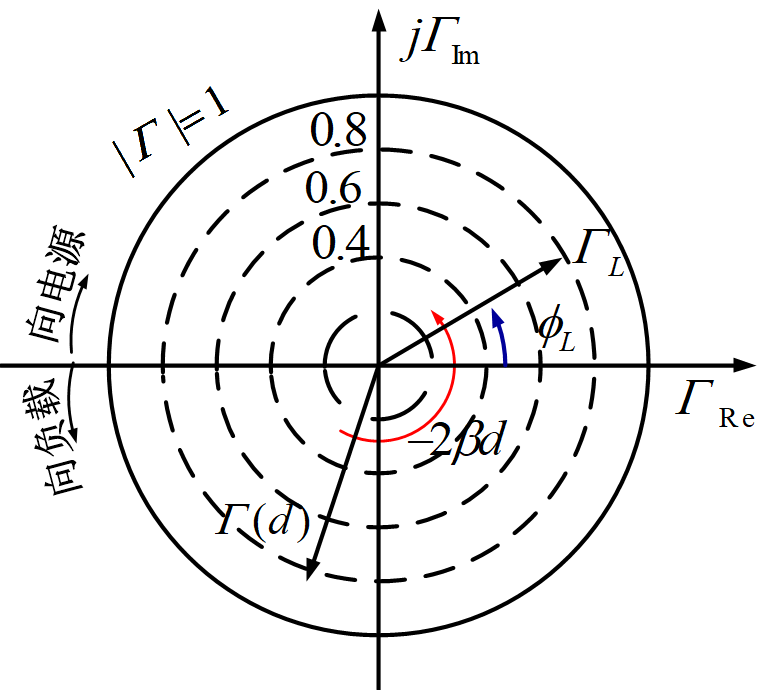
\includegraphics[width=6cm]{reflect_coeff.png}
    \caption{反射系数圆}
   \end{figure}
  \end{column}
 \end{columns}
\end{frame}

\begin{frame}{Smith Chart(阻抗圆图及其应用)}
 \textbf{相角相等的反射系数的轨迹是单位圆内的径向线}
 \begin{columns}
  \begin{column}{0.4\linewidth}
   线上移动长度$\lambda/2$时,对应反射系数矢量转动一周。一般转动的角度用波长数(或电长度)$\Delta d/\lambda$表示,且标度波长数的零点位置通常选在$\phi=\pi$处。
  \end{column}
  \begin{column}{0.6\linewidth}
   \begin{figure}
    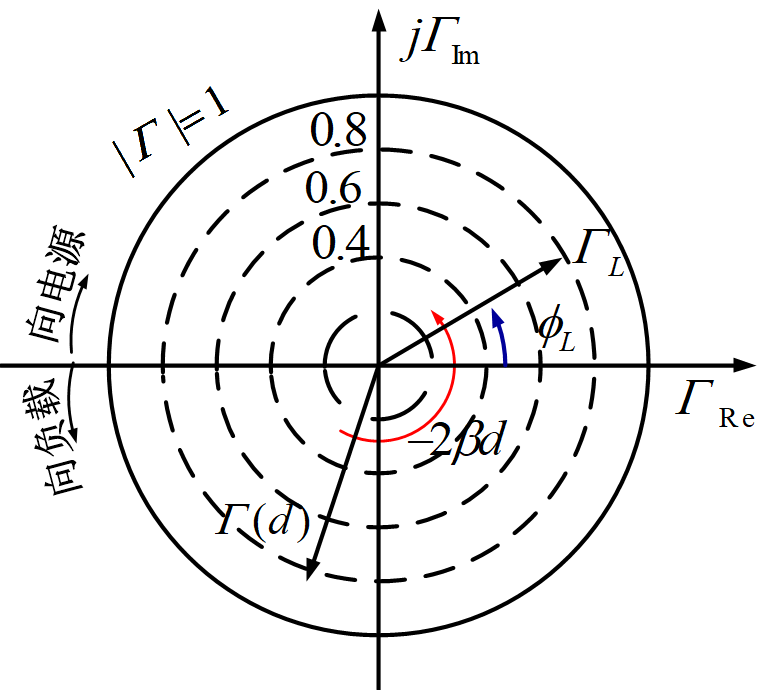
\includegraphics[width=4cm]{reflect_coeff.png}
    \caption{等反射系数圆的波长数标度}
   \end{figure}
  \end{column}
 \end{columns}
 $\phi=0$\textbf{的径向线为各种不同负载阻抗情况下电压波腹点反射系数的轨迹;}\\
 $\phi=\pi$\textbf{的径向线为各种不同负载阻抗情况下电压波节点反射系数的轨迹。}
\end{frame}

\begin{frame}{Smith Chart(阻抗圆图及其应用)}
 \begin{itemize}
  \item 阻抗圆图
        \begin{enumerate}
         \resume
         \item 归一化阻抗圆
        \end{enumerate}
        \begin{empheq}[box=\widefbox]{align*}
         z_{in}(d)=\frac{Z_{in}(d)}{Z_0}=\frac{1+\Gamma(d)}{1-\Gamma(d)}
        \end{empheq}
 \end{itemize}
 \begin{align*}
  z_{in}(d) & =\frac{1+(\Gamma_{Re}+j\Gamma_{Im})}{1-(\Gamma_{Re}+j\Gamma_{Im})}                                                                          \\
            & =\frac{1-(\Gamma^{2}_{Re}+\Gamma^{2}_{Im})}{(1-\Gamma_{Re})^2+\Gamma_{Im}^{2}}+j\frac{2\Gamma_{Im}}{(1-\Gamma_{Re})^2+\Gamma_{Im}^{2}}=r+jx
 \end{align*}
 \begin{empheq}[box=\widefbox]{align*}
  \left(\Gamma_{Re}-\frac{r}{r+1}\right)^2+\Gamma_{Im}^{2}=\frac{1}{(r+1)^2}\quad \text{归一化电阻轨迹方程}\\
  (\Gamma_{Re}-1)^2+\left(\Gamma_{Im}-\frac{1}{x}\right)^2=\left(\frac{1}{x}\right)^2\quad \text{归一化电抗轨迹方程}
 \end{empheq}
 \footnotesize{特征参数,是形成统一Smith圆图的最关键点,它包含了阻抗归一和电长度归一。}
\end{frame}

\begin{frame}{Smith Chart(阻抗圆图及其应用)}
  \only<1>{\begin{columns}
    \begin{column}{0.55\linewidth}
      \begin{empheq}[box=\widefbox]{align*}
        (\Gamma_{Re}-1)^2+\left(\Gamma_{Im}-\frac{1}{x}\right)^2=\left(\frac{1}{x}\right)^2
      \end{empheq}
    \end{column}
    \begin{column}{0.45\linewidth}
      \begin{figure}
        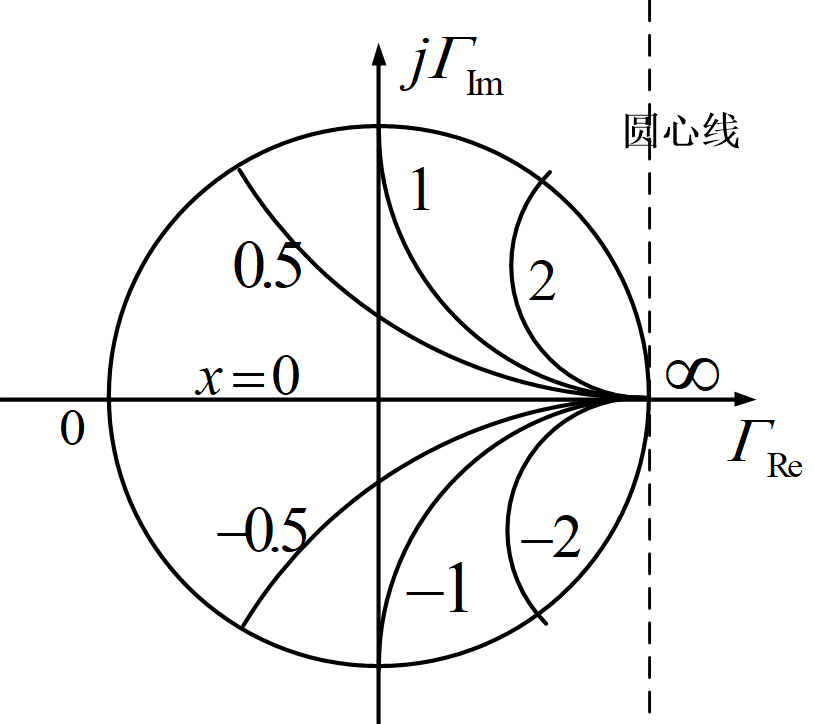
\includegraphics[width=5cm]{diankangyuan.png}
        \caption{归一化电抗圆}
      \end{figure}
    \end{column}
  \end{columns}}
  \only<2>{\begin{columns}
    \begin{column}{0.45\linewidth}
      \begin{figure}
        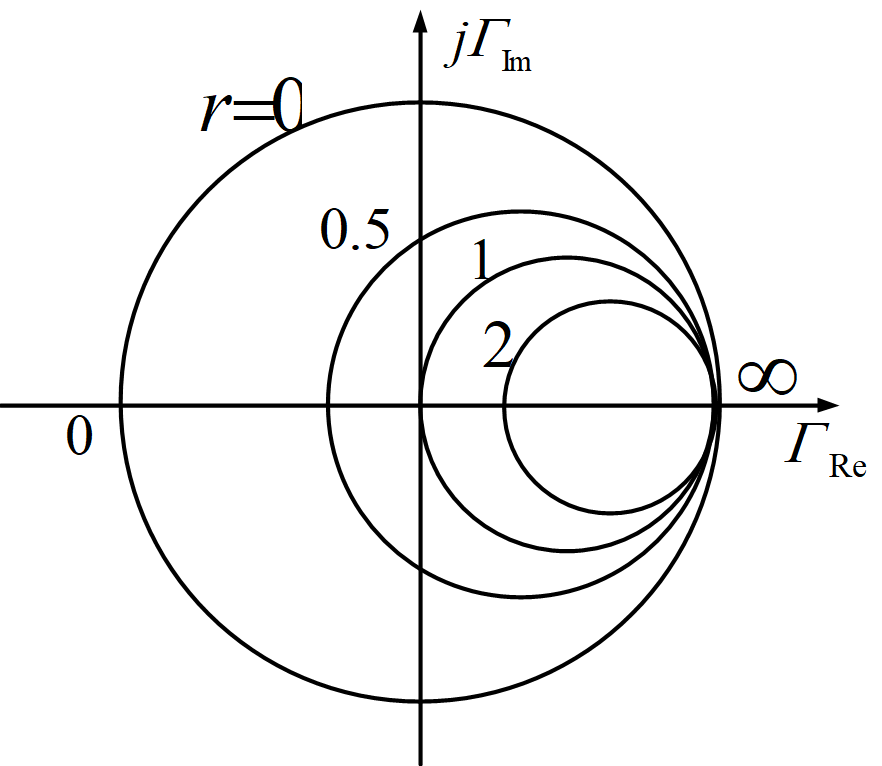
\includegraphics[width=5cm]{dianzuyuan.png}
        \caption{归一化电阻圆}
      \end{figure}
    \end{column}
    \begin{column}{0.55\linewidth}
      \begin{empheq}[box=\widefbox]{align*}
        \left(\Gamma_{Re}-\frac{r}{r+1}\right)^2+\Gamma_{Im}^2=\frac{1}{(r+1)^2}
      \end{empheq}
    \end{column}
  \end{columns}}
\end{frame}

\begin{frame}{Smith Chart(阻抗圆图及其应用)}
  电阻圆始终和直线$\Gamma_r=1$相切
  \begin{columns}
    \begin{column}{0.42\linewidth}
      \begin{figure}
        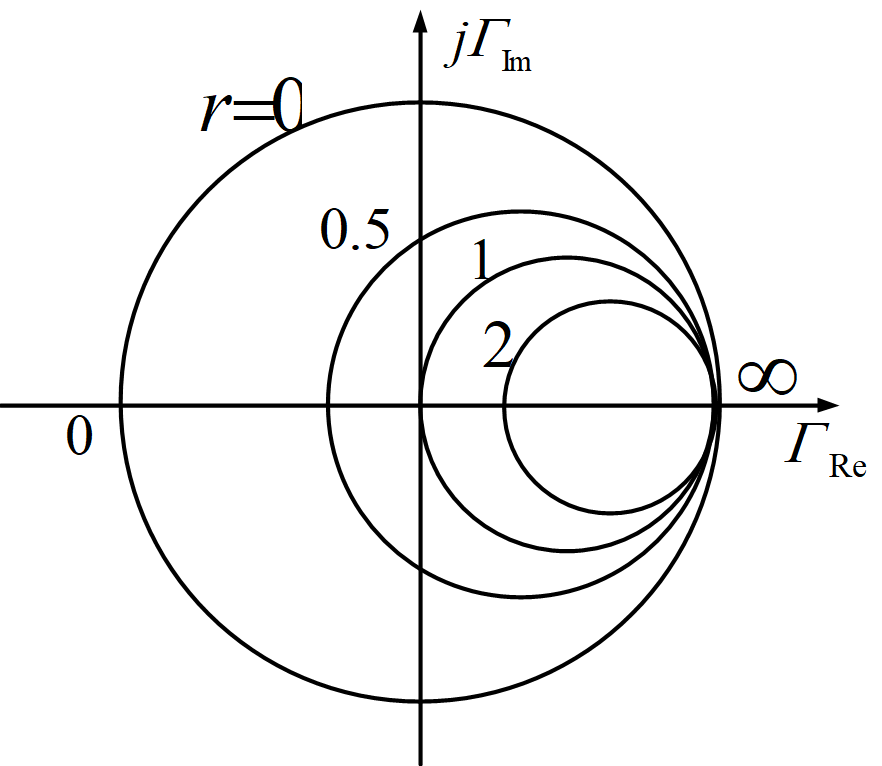
\includegraphics[width=4.55cm]{dianzuyuan.png}
        \caption{归一化电阻圆}
      \end{figure}
    \end{column}
    \begin{column}{0.58\linewidth}
      \begin{tabular}{|c|c|c|c|}
        \hline
        \multirow{2}*{$r$} &
        \multicolumn{2}{c|}{\footnotesize{圆心坐标}} &
        \multirow{2}*{\footnotesize{半径} $\left(\frac{1}{1+r}\right)$}\\ \cline{2-3}
        & $\Gamma_r=\frac{r}{1+r}$ & $\Gamma_i=0$ \\ \hline
        0 & 0 & 0 & 1 \\ \hline
        1 & 1/2 & 0 & 1/2 \\ \hline
        2 & 2/3 & 0 & 1/3 \\ \hline
      \end{tabular}
    \end{column}
  \end{columns}
  \begin{empheq}[box=\widefbox]{align*}
    \left(\Gamma_{Re}-\frac{r}{r+1}\right)^2+\Gamma_{Im}^2=\frac{1}{(r+1)^2}
  \end{empheq}
\end{frame}

\begin{frame}{Smith Chart(阻抗圆图及其应用)}
  电抗圆圆心坐标和半径
  \begin{empheq}[box=\widefbox]{align*}
      (\Gamma_{Re}-1)^2+\left(\Gamma_{Im}-\frac{1}{x}\right)^2=\left(\frac{1}{x}\right)^2
  \end{empheq}
  \begin{columns}
    \begin{column}{0.58\linewidth}
      \begin{tabular}{|c|c|c|c|}
        \hline
        \multirow{2}*{$x$} &
        \multicolumn{2}{c|}{\footnotesize{圆心坐标}} &
        \multirow{2}*{\footnotesize{半径} $\left(\frac{1}{x}\right)$}\\ \cline{2-3}
        & $\Gamma_r=1$ & $\Gamma_i=\frac{1}{x}$ \\ \hline
        0 & 1 & \infty & \infty \\ \hline
        \pm0.5 & 1 & \pm2 & 2 \\ \hline
        \pm1 & 1 & \pm1 & 1 \\ \hline
      \end{tabular}
    \end{column}
    \begin{column}{0.42\linewidth}
      \begin{figure}
        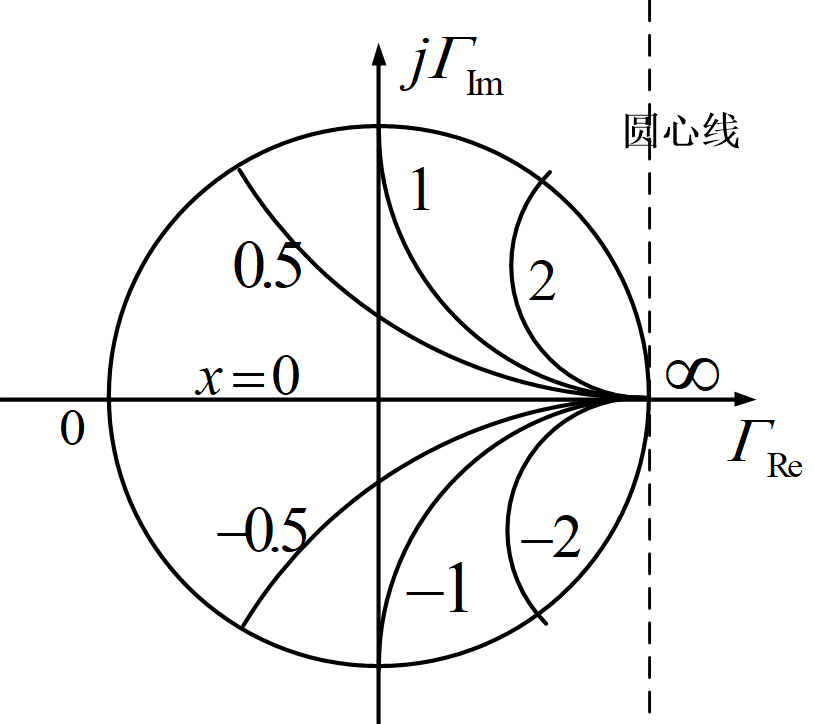
\includegraphics[width=4.55cm]{diankangyuan.png}
        \caption{归一化电抗圆}
      \end{figure}
    \end{column}
  \end{columns}
\end{frame}

\begin{frame}{Smith Chart(阻抗圆图及其应用)}
  将等电阻圆和等电抗圆绘制在同一张图上,得到阻抗圆图。
  \centering
  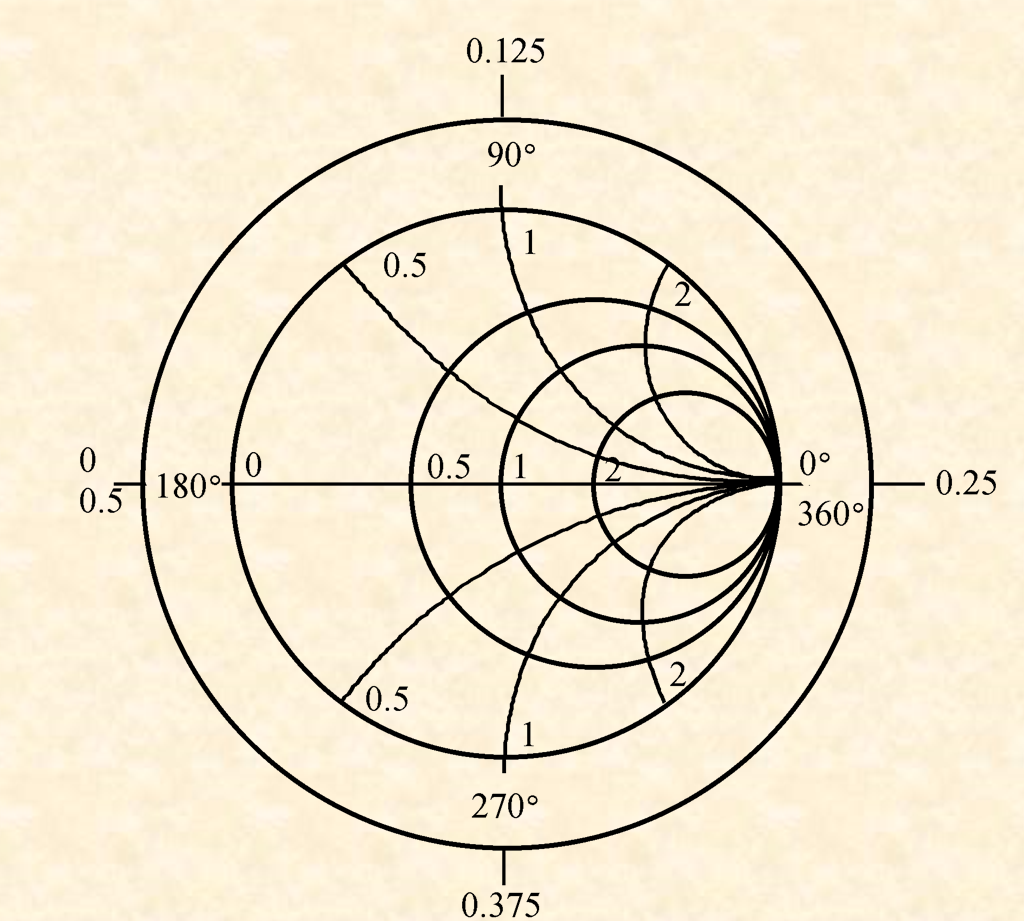
\includegraphics[width=8cm]{zukangyuan.png}
\end{frame}

\begin{frame}{Smith Chart(阻抗圆图及其应用)}
  阻抗圆图有如下几个特点
  \begin{columns}
    \begin{column}{0.4\linewidth}
      (1)圆图上有三个特殊点:\\
      \textbf{匹配点}(O点),其坐标为(0,0)\\
      $r=1,x=0$ \\
      $\lvert\Gamma\rvert=0,\rho=1$\\
      \textbf{短路点}(C点),其坐标为(-1,0)\\
      $r=0,x=0,\lvert\Gamma\rvert=1$ \\
      $\rho=\infty,\phi=\pi$ \\
      \textbf{开路点}(D点),其坐标为(1,0)\\
      $r=\infty,x=\infty,\lvert\Gamma\rvert=1$ \\
      $\rho=\infty,\phi=0$
    \end{column}
    \begin{column}{0.6\linewidth}
      \only<1>{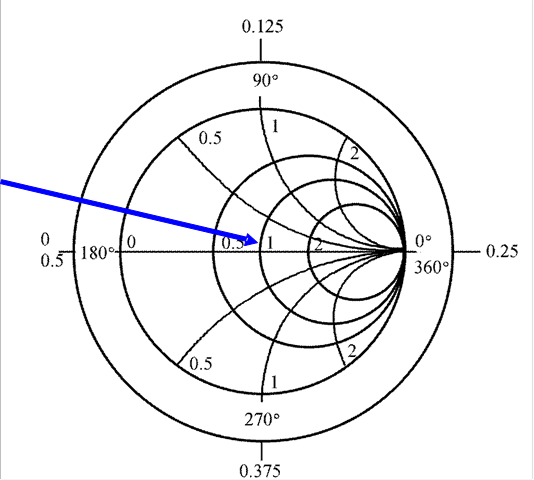
\includegraphics[width=5cm]{smithchart-1.png}}
      \only<2>{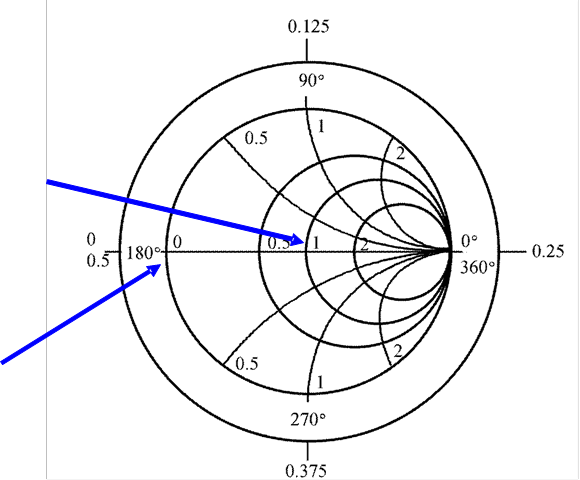
\includegraphics[width=5cm]{smithchart-2.png}}
      \only<3>{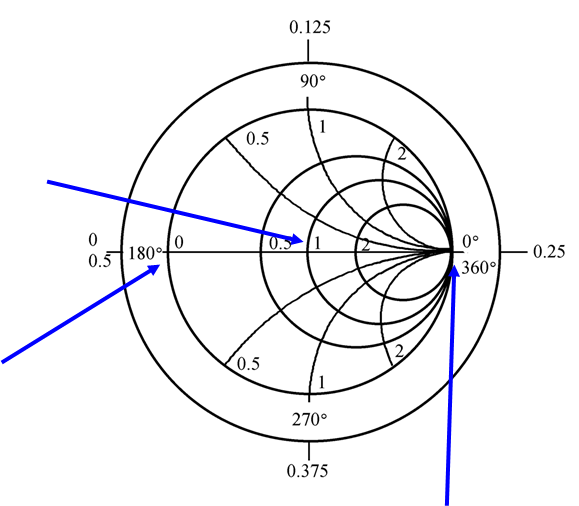
\includegraphics[width=5cm]{smithchart-3.png}}
    \end{column}
  \end{columns}
\end{frame}

\begin{frame}{Smith Chart(阻抗圆图及其应用)}
  \begin{columns}
    \begin{column}{0.4\linewidth}
      (2)圆图上有三条特殊线\\
      圆图上实轴为$x=0$的轨迹,\\正半实轴为电压波腹点的轨迹,\\线上$R$值为驻波比读数。\\
      负半实轴为电压波节点的轨迹,\\
      线上的$R$值为行波系数$K$的\\
      读数。\\
      最外面的单位圆为$R=0$的纯\\
      电抗轨迹,即为$\lvert\Gamma\rvert=1$的全反射\\
      系数圆的轨迹.
    \end{column}
    \begin{column}{0.6\linewidth}
      \only<1>{\includegraphics[width=5cm]{smithchart-4.png}}
      \only<2>{\includegraphics[width=5cm]{smithchart-5.png}}
      \only<3>{\includegraphics[width=5cm]{smithchart-6.png}}
    \end{column}
  \end{columns}
\end{frame}

\begin{frame}{Smith Chart(阻抗圆图及其应用)}
 例1 \quad 特性阻抗$Z_0=50\Omega$,负载阻抗$Z_L=100+j50\Omega$,求距负载$0.24\lambda$处输入阻抗。\\
 解:归一化负载阻抗$z_L=2+j1$\\
 \begin{columns}
  \begin{column}{0.5\linewidth}
   1)\quad 向电源方向旋转$0.213\lambda$
   \begin{align*}
    \phi=\arctan(1/2)                         \\
    \frac{2\pi}{\lambda/2}=\frac{\pi-\phi}{l} \\
    l =(\pi-0.4636)\lambda/4\pi               \\
    =0.213\lambda
   \end{align*}
   2)\quad 旋转$0.24\lambda$到$z_{in}$
   \begin{align*}
    z_in=0.42-j0.25\rightarrow\times 50 \\
    \rightarrow 21-j12.5\Omega
   \end{align*}
  \end{column}
  \begin{column}{0.5\linewidth}
   \only<1>{\includegraphics[width=5cm]{example1-1.png}}
   \only<2>{\includegraphics[width=5cm]{example1-2.png}}
   \only<3>{\includegraphics[width=5cm]{example1-3.png}}
   \only<4>{\includegraphics[width=5cm]{example1-4.png}}
   \only<5>{\includegraphics[width=5cm]{example1-5.png}}
   \only<6>{\includegraphics[width=5cm]{example1-6.png}}
   \only<7>{\includegraphics[width=5cm]{example1-7.png}}
   \only<8>{\includegraphics[width=5cm]{example1-8.png}}
   \only<9>{\includegraphics[width=5cm]{example1-9.png}}
   \only<10>{\includegraphics[width=5cm]{example1-10.png}}
   \only<11>{\includegraphics[width=5cm]{example1-11.png}}
  \end{column}
 \end{columns}
\end{frame}

\subsection{传输线的阻抗匹配}
\begin{frame}{传输线的阻抗匹配}

\end{frame}

%\section{第3章\quad 分布电路与传输线理论}


\begin{frame}{传输线理论}
 \begin{itemize}
  \item \textbf{传输线理论,一维分布参数电路理论,微波电路设计和计算的理论基础。}
  \item \textbf{传输线理论,电路理论与场的理论之间起着桥梁的作用。}
 \end{itemize}
\end{frame}

\subsection{传输线方程}
\begin{frame}{传输线方程}
 \begin{enumerate}
  \item 传输线的电路模型
 \end{enumerate}
 \centering
 \includegraphics[width=9cm]{guidesystem.png}
 \saveenum
\end{frame}


\begin{frame}{传输线方程}
 \textbf{传输线}是以TEM导模的方式传送电磁波能量或信号的导行系统,其横向尺寸远小于其上工作波长。\\
 \textbf{传输线}有\textbf{长线}和\textbf{短线}之分。所谓长线是指传输线的几何长度与线上传输电磁波的波长比值(电长度)可相比拟,反之称为短线。\\
 \begin{align*}
  \text{长线}\Longrightarrow\text{分布参数电路} \\
  \text{短线}\Longrightarrow\text{集中参数电路} \\
  \text{分界线:}\widefbox{$l/\lambda\geq 0.05$}
 \end{align*}
 当频率提高到微波波段时,这些分布效应不可忽略,所以微波传输线是一种\textbf{分布参数电路}。这导致传输线上的电压和电流是随时间和空间位置而变化的二元函数。
\end{frame}

\begin{frame}{传输线方程}
 根据传输线上的分布参数是否均匀分布,可将其分为均匀传输线和不均匀传输线。我们可以把均匀传输线分割成许多小的微元段$dz(dz<<\lambda)$,这样每个微元段可以看作集中参数电路,用一个$\Gamma$型网络来等效。于是整个传输线可等效成无穷多个$\Gamma$型网络的级联。\\
 \centering
 \includegraphics[width=9cm]{transmissionline1.png}
\end{frame}


\begin{frame}{传输线方程}
 双导线、同轴线和平行线传输线的分布参数\\
 \centering
 \includegraphics[width=9cm]{tmlineparas.png}
\end{frame}

\begin{frame}{传输线方程}
 \begin{enumerate}
  \resume
  \item 传输线方程\\
        \begin{itemize}
         \item 一般传输线方程或电报方程\\
               \includegraphics[width=6cm]{transmissionline2.png}
        \end{itemize}
        \saveenum
 \end{enumerate}
 \flushleft
 \fbox{$ v(z+\Delta z,t)=v(z,t)+\frac{\partial v(z,t)}{\partial z}\Delta z $}
 \flushright
 \fbox{$ i(z+\Delta z,t)=i(z,t)+\frac{\partial i(z,t)}{\partial z}\Delta z $}\\
 \begin{align*}
  f(x)=f(x_{0})+f^{'}(x_{0})(x-x_{0})  +\frac{f^{''}(x_{0})}{2!}(x-x_{0})^{2}+\ldots \\
  +\frac{f^{n}(x_{0})}{n!}(x-x_{0})^{n}+R_{n}(x)
 \end{align*}
\end{frame}

\begin{frame}{传输线方程}
 \centering
 \includegraphics[width=7cm]{transmissionline2.png}
 \flushleft
 线元$\Delta z$上的电压、电流的变化为:
 \begin{empheq}[box=\widefbox]{align*}
  v(z,t)-v(z+\Delta z,t)=-\frac{\partial v(z,t)}{\partial z}\Delta z\\
  i(z,t)-i(z+\Delta z,t)=-\frac{\partial i(z,t)}{\partial z}\Delta z
 \end{empheq}
\end{frame}

\begin{frame}{传输线方程}
 \centering
 \includegraphics[width=7cm]{transmissionline2.png}
 \flushleft
 线元$\Delta z$上应用基尔霍夫定律,可得:
 \begin{empheq}[box=\widefbox]{align*}
  -\frac{\partial v(z,t)}{\partial z}\Delta z=R_{1}\Delta z\cdot i(z,t)+L_{1}\Delta z\cdot\frac{\partial i(z,t)}{\partial t}\\
  -\frac{\partial i(z,t)}{\partial z}\Delta z=G_{1}\Delta z\cdot v(z,t)+C_{1}\Delta z\cdot\frac{\partial v(z,t)}{\partial t}
 \end{empheq}
\end{frame}

\begin{frame}{传输线方程}
 \begin{empheq}[box=\widefbox]{align*}
  -\frac{\partial v(z,t)}{\partial z}\Delta z=R_{1}\Delta z\cdot i(z,t)+L_{1}\Delta z\cdot\frac{\partial i(z,t)}{\partial t}\\
  -\frac{\partial i(z,t)}{\partial z}\Delta z=G_{1}\Delta z\cdot v(z,t)+C_{1}\Delta z\cdot\frac{\partial v(z,t)}{\partial t}
 \end{empheq}
 \flushleft
 令$\Delta z \rightarrow 0$
 \begin{empheq}[box=\widefbox]{align*}
  \frac{\partial v(z,t)}{\partial z}=-R_{1}\cdot i(z,t)-L_{1}\cdot\frac{\partial i(z,t)}{\partial t}\\
  \frac{\partial i(z,t)}{\partial z}=-G_{1}\cdot v(z,t)-C_{1}\cdot\frac{\partial v(z,t)}{\partial t}
 \end{empheq}
 \centering
 \textbf{一般传输线方程、电报方程}
\end{frame}

\begin{comment}
\newcommand{\mtikzmark}[1]{\tikz[overlay,remember picture]\node(#1){};}
\tikzset{mylabel/.style={align=center,fill=blue!10,font=\footnotesize}}
%\mytlabel[options]{start.mark}{end.mark}{text}

\newcommand\mytlabel[4][]{%
 \tikz[overlay,remember picture]
 {\draw[->]([yshift=-10pt]#2.north) -- node[mylabel,#1]{#4}([yshift=6pt]#3.north);}
}
\end{comment}

\begin{frame}{传输线方程}
 \begin{itemize}
  \item 时谐均匀传输线方程
 \end{itemize}
 \begin{empheq}[box=\widefbox]{align*}
  \frac{\partial v(z,t)}{\partial z}=-R_{1}\cdot i(z,t)-L_{1}\cdot\frac{\partial i(z,t)}{\partial t}\\
  \frac{\partial i(z,t)}{\partial z}=-G_{1}\cdot v(z,t)-C_{1}\cdot\frac{\partial v(z,t)}{\partial t}
 \end{empheq}
 \begin{columns}
  \begin{column}{0.5\linewidth}
   \begin{empheq}[box=\widefbox]{align*}
    v(z,t)=Re\left[V(z)e^{j\omega t}\right]\\
    i(z,t)=Re\left[I(z)e^{j\omega t}\right]
   \end{empheq}
  \end{column}
  \begin{column}{0.5\linewidth}
   分布参数:$R_{1}$,$L_{1}$,$C_{1}$,$G_{1}$不随位置变化
  \end{column}
 \end{columns}
\end{frame}

\begin{frame}{传输线方程}
 \begin{empheq}[box=\widefbox]{align*}
  \frac{dV(z)}{dz}=-(R_{1}+j\omega L_{1})I(z)=-Z_{1}I(z)\\
  Z_{1}=R_{1}+j\omega L_{1} \text{:单位长度串联阻抗}
 \end{empheq}
 \begin{empheq}[box=\widefbox]{align*}
  \frac{dI(z)}{dz}=-(G_{1}+j\omega C_{1})V(z)=-Y_{1}V(z)\\
  Y_{1}=G_{1}+j\omega C_{1} \text{:单位长度并联导纳}
 \end{empheq}
 对$z$再微商
 \begin{align*}
  \frac{d^2}{dz^2}\left\{
  \begin{aligned}
   V(z) \\I(z)
  \end{aligned}
  \right\}-\gamma^2
  \left\{\begin{aligned}
          V(z) \\I(z)
         \end{aligned}\right\}=0
 \end{align*}
 \textbf{电压传播常数}:\fbox{$\gamma=\sqrt{Z_{1}Y_{1}}=\sqrt{(R_{1}+j\omega L_{1})(G_{1}+j\omega C_{1})}$}
\end{frame}


\begin{frame}{传输线方程}
 \begin{itemize}
  \item 时谐传输线方程电压、电流通解
 \end{itemize}
 电压:
 \begin{empheq}[box=\widefbox]{align*}
  V(z)=A_{1}e^{-\gamma z}+A_{2}e^{\gamma z}
 \end{empheq}
 电流:
 \begin{empheq}[box=\widefbox]{align*}
  I(z)=-\frac{1}{R_{1}+j\omega L_{1}}\frac{dV(z)}{dz}=\frac{1}{Z_{0}}(A_{1}e^{-\gamma z}-A_{2}e^{\gamma z})
 \end{empheq}
 $$\gamma=\sqrt{Z_{1}Y_{1}}=\sqrt{(R_{1}+j\omega L_{1})(G_{1}+j\omega C_{1})}$$
 \textbf{特性阻抗}:
 \begin{empheq}[box=\widefbox]{align*}
  Z_{0}=\sqrt{\frac{R_{1}+j\omega L_{1}}{G_{1}+j\omega C_{1}}}
 \end{empheq}
\end{frame}

\begin{frame}{传输线方程}
 \begin{itemize}
  \item 传输线方程的边界条件和解
 \end{itemize}
 \begin{columns}
  \begin{column}{0.35\linewidth}
   端接条件确定常数:\\
   终端条件\\
   始端条件\\
   信号源和负载条件
  \end{column}
  \begin{column}{0.65\linewidth}
   \includegraphics[width=6cm]{tmlineboundary.png}
  \end{column}
 \end{columns}
 \textbf{终端条件}解:
 \begin{columns}
  \begin{column}{0.5\linewidth}
   \begin{empheq}[box=\widefbox]{align*}
    V(z)=A_{1}e^{-\gamma z}+A_{2}e^{\gamma z}
   \end{empheq}
  \end{column}
  \begin{column}{0.5\linewidth}
   \begin{empheq}[box=\widefbox]{align*}
    I(z)=(A_{1}e^{-\gamma z}-A_{2}e^{\gamma z})/Z_{0}
   \end{empheq}
  \end{column}
 \end{columns}
 \begin{empheq}[box=\widefbox]{align*}
  V(l)=V_{L}=A_{1}e^{-\gamma l}+A_{2}e^{\gamma l}\\
  I(l)=I_{L}=\frac{1}{Z_{0}}(A_{1}e^{-\gamma l}-A_{2}e^{\gamma l})
 \end{empheq}
\end{frame}


\begin{frame}{传输线方程}
 \begin{empheq}[box=\widefbox]{align*}
  A_{1}=\frac{V_{L}+I_{L}Z_{0}}{2}e^{\gamma l},A_{2}=\frac{V_{L}-I_{L}Z_{0}}{2}e^{-\gamma l}
 \end{empheq}
 代入:
 \begin{columns}
  \begin{column}{0.45\linewidth}
   \begin{empheq}[box=\widefbox]{align*}
    V(z)=A_{1}e^{-\gamma z}+A_{2}e^{\gamma z}
   \end{empheq}
  \end{column}
  \begin{column}{0.45\linewidth}
   \begin{empheq}[box=\widefbox]{align*}
    I(z)=(A_{1}e^{-\gamma z}-A_{2}e^{\gamma z})/Z_{0}
   \end{empheq}
  \end{column}
 \end{columns}
 对于终端边界条件场合,我们常采用$d$(终端出发)坐标系$d$,换坐标\fbox{$d=l-z$}
 \begin{empheq}[box=\widefbox]{align*}
  V(d)=\frac{V_{L}+I_{L}Z_{0}}{2}e^{\gamma d}+\frac{V_{L}-I_{L}Z_{0}}{2}e^{-\gamma d}=V^{+}(d)+V^{-}(d)\\
  I(d)=\frac{V_{L}+I_{L}Z_{0}}{2Z_{0}}e^{\gamma d}-\frac{V_{L}-I_{L}Z_{0}}{2Z_{0}}e^{-\gamma d}=I^{+}(d)+I^{-}(d)
 \end{empheq}
\end{frame}

\begin{frame}{传输线方程}
 \begin{empheq}[box=\widefbox]{align*}
  V(d)=\frac{V_{L}+I_{L}Z_{0}}{2}e^{\gamma d}+\frac{V_{L}-I_{L}Z_{0}}{2}e^{-\gamma d}=V^{+}(d)+V^{-}(d)\\
  I(d)=\frac{V_{L}+I_{L}Z_{0}}{2Z_{0}}e^{\gamma d}-\frac{V_{L}-I_{L}Z_{0}}{2Z_{0}}e^{-\gamma d}=I^{+}(d)+I^{-}(d)
 \end{empheq}
 \begin{empheq}[box=\widefbox]{align*}
  V(d)=\frac{e^{\gamma d}+e^{-\gamma d}}{2}V_{L}+\frac{e^{\gamma d}-e^{-\gamma d}}{2}Z_{0}I_{L}\\
  I(d)=\frac{e^{\gamma d}+e^{-\gamma d}}{2}\frac{1}{Z_{0}}V_{L}+\frac{e^{\gamma d}-e^{-\gamma d}}{2}I_{L}
 \end{empheq}
 \begin{align*}
  \begin{bmatrix}
   V(d) \\I(d)
  \end{bmatrix}
  =
  \begin{bmatrix}
   \cosh\gamma d           & Z_{0}\sinh\gamma d \\
   Z_{0}^{-1}\sinh\gamma d & \cosh\gamma d
  \end{bmatrix}
  \begin{bmatrix}
   V_{L} \\I_{L}
  \end{bmatrix}
 \end{align*}
\end{frame}


\begin{frame}{传输线方程}
 \textbf{始端条件解}:已知始端电压和电流$V_{0},I_{0}$ \\
 \fbox{$V(z)=A_{1}e^{-\gamma z}+A_{2}e^{\gamma z}$}
 \fbox{$I(z)=(A_{1}e^{-\gamma z}-A_{2}e^{\gamma z})/Z_{0}$}\\
 \begin{columns}
  \begin{column}{0.3\linewidth}
   \begin{align*}
    V_{0}=A_{1}+A_{2} \\
    I_{0}=(A_{1}-A_{2})/Z_{0}
   \end{align*}
  \end{column}
  \begin{column}{0.1\linewidth}
   \centering
   $ \longrightarrow $
  \end{column}
  \begin{column}{0.6\linewidth}
   \begin{empheq}[box=\fbox]{align*}
    A_{1}=\frac{V_{0}+I_{0}Z_{0}}{2}\quad A_{2}=\frac{V_{0}-I_{0}Z_{0}}{2}
   \end{empheq}
  \end{column}
 \end{columns}
 \begin{empheq}[box=\widefbox]{align*}
  V(z)=\frac{V_{0}+I_{0}Z_{0}}{2}e^{-\gamma z}+\frac{V_{0}-I_{0}Z_{0}}{2}e^{\gamma z}\\
  I(z)=\frac{V_{0}+I_{0}Z_{0}}{2Z_{0}}e^{-\gamma z}+\frac{V_{0}-I_{0}Z_{0}}{2Z_{0}}e^{\gamma z}
 \end{empheq}
 \begin{align*}
  \begin{bmatrix}
   V(z) \\I(z)
  \end{bmatrix}
  =
  \begin{bmatrix}
   \cosh\gamma z            & -Z_{0}\sinh\gamma z \\
   -Z_{0}^{-1}\sinh\gamma z & \cosh\gamma z
  \end{bmatrix}
  \begin{bmatrix}
   V_{0} \\I_{0}
  \end{bmatrix}
 \end{align*}
\end{frame}

\begin{frame}{传输线方程}
 \textbf{信号源和负载条件解}:
 已知信号源电动势 $E_{G}$、
 内阻抗 $Z_{G}$、
 负载阻抗 $Z_{L}$
 \begin{empheq}[box=\widefbox]{align*}
  V(d)=\frac{E_{G}Z_{0}}{Z_{G}+Z_{0}}\cdot\frac{e^{-\gamma l}}{1-\Gamma_{L}\Gamma_{G}e^{-2\gamma l}}(e^{\gamma d}+\Gamma_{L}e^{-\gamma d})\\
  I(d)=\frac{E_{G}}{Z_{G}+Z_{0}}\cdot\frac{e^{-\gamma l}}{1-\Gamma_{L}\Gamma_{G}e^{-2\gamma l}}(e^{\gamma d}-\Gamma_{L}e^{-\gamma d})
 \end{empheq}
 \begin{align*}
  \Gamma_{L}=\frac{Z_{L}-Z_{0}}{Z_{L}+Z_{0}}\quad \Gamma_{G}=\frac{Z_{G}-Z_{0}}{Z_{G}+Z_{0}}\quad\text{反射系数}
 \end{align*}
\end{frame}

\begin{frame}{传输线方程}
 \begin{enumerate}
  \resume
  \item \textbf{传输线的特性参数}
        \begin{itemize}
         \item 特性阻抗
        \end{itemize}
        \begin{align*}
         Z_{0}=\sqrt{\frac{R_{1}+j\omega L_{1}}{G_{1}+j\omega C_{1}}}
        \end{align*}
        传输线上\textbf{行波}的电压与电流之比称为传输线的特性阻抗\\
        $$\text{无耗线}R_{1}=G_{1}=0\quad Z_{0}=\sqrt{\frac{L_{1}}{C_{1}}}$$\\
        微波低耗线$R_{1}<<\omega L_{1},G_{1}<<\omega C_{1}$\\
        $$Z_{0}=\sqrt{\frac{R_{1}+j\omega L_{1}}{G_{1}+j\omega C_{1}}}\approx\sqrt{\frac{L_{1}}{C_{1}}}\left[1+\frac{1}{2}\left(\frac{R_{1}}{j\omega L_{1}}-\frac{G_{1}}{j\omega C_{1}}\right)\right]$$
 \end{enumerate}
\end{frame}

\begin{frame}{传输线方程}
 \begin{itemize}
  \item \textbf{双导线特性阻抗}\\
        $$Z_{0}=120\ln\left[\frac{D}{d}+\sqrt{\left(\frac{D}{d}\right)^{2}-1}\right]$$
  \item \textbf{同轴线特性阻抗}\\
        $$Z_{0}=\frac{60}{\sqrt{\epsilon_{r}}}\ln\frac{b}{a}$$
  \item \textbf{平行板传输线特性阻抗}\\
        $$Z_{0}=\frac{d}{W}\eta$$
 \end{itemize}
\end{frame}

\begin{frame}{传输线方程}
 \begin{itemize}
  \item \textbf{传播常数}
 \end{itemize}
 描述导行波沿着导行系统传播过程中的\textbf{衰减和相位变化}的参数
 \begin{empheq}[box=\widefbox]{align*}
  \gamma = \sqrt{(R_{1}+j\omega L_{1})(G_{1}+j\omega C_{1})}=\alpha+j\beta
 \end{empheq}
 $\alpha$——衰减常数,单位$Np/m$或$dB/m$\quad $(1Np=8.686dB)$\\
 $\beta$——相位常数,单位$rad/m$\\
 \centering
 $\text{无耗线}\quad \alpha=0$\quad \fbox{$\beta=\omega\sqrt{L_{1}C_{1}}$}
\end{frame}

\begin{frame}{传输线方程}
 微波低耗线\quad$R_{1}<<\omega L_{1},G_{1}<<\omega C_{1}$
 \begin{align*}
  \gamma & =\sqrt{(R_{1}+j\omega L_{1})(G_{1}+j\omega C_{1})}=\alpha+j\beta                                                \\
         & =\sqrt{(j\omega)^{2}L_{1}C_{1}}\sqrt{\left(1+\frac{R_{1}}{j\omega L_{1}}\right)(1+\frac{G_{1}}{j\omega C_{1}})} \\
         & \approx\frac{1}{2}\left(R_{1}\sqrt{C_{1}/L_{1}}+G_{1}\sqrt{L_{1}/C_{1}}\right)+j\omega\sqrt{L_{1}C_{1}}
 \end{align*}
 \begin{columns}
  \begin{column}{0.65\linewidth}
   \begin{empheq}[box=\widefbox]{align*}
    \therefore\alpha=\frac{R_{1}}{2Z_{0}}+\frac{G_{1}Z_{0}}{2}=\alpha_{c}+\alpha_{d}
   \end{empheq}
   $\alpha_{c}$:分布电阻产生的导体衰减常数\\
   $\alpha_{d}$:漏电导产生的介质衰减常数
  \end{column}
  \begin{column}{0.35\linewidth}
   \begin{empheq}[box=\widefbox]{align*}
    \therefore\beta=\omega\sqrt{L_{1}C_{1}}
   \end{empheq}
   $\beta$:近似于无耗传输线的相位常数
  \end{column}
 \end{columns}
\end{frame}

\begin{frame}{传输线方程}
 对于TEM导波:\\
 $$k_{c}=0,\lambda_{c}=\infty$$\\
 其相速度为\\
 $$v_{p}=v=\frac{\omega}{\beta}=\frac{1}{\sqrt{L_{1}C_{1}}}$$\\
 波长为\\
 $$\lambda_{g}=\lambda=\frac{2\pi}{\beta}=\frac{v_{p}}{f}$$\\
 特性阻抗为\\
 $$Z_{0}=\sqrt{\frac{L_{1}}{C_{1}}}=\frac{1}{v_{p}C_{1}}=v_{p}L_{1}$$\\
 \textbf{传输线的特性阻抗可由单位长度分布电容或分布电感求得}
\end{frame}


\subsection{分布参数阻抗}
\begin{frame}{分布参数阻抗}
 \begin{itemize}
  \item 微波阻抗——由微波传输线上的电压和电流决定的,是\textbf{分布参数}阻抗。(低频传输线阻抗是\textbf{集中参数}阻抗)
  \item 微波阻抗——与导行系统上导波的反射或者驻波特性密切相关,即与导行系统的状态或者特性密切相关。
  \item 微波阻抗不能直接测量,需要借助反射参量或者驻波参量的直接测量而间接获得。
 \end{itemize}
\end{frame}

\begin{frame}{分布参数阻抗}
 \begin{enumerate}
  \item \textbf{分布参数阻抗}
        \saveenum
 \end{enumerate}
 \centering
 \includegraphics[width=8cm]{tmlineboundary.png}
 \begin{align*}
  \begin{bmatrix}
   V(d) \\I(d)
  \end{bmatrix}=
  \begin{bmatrix}
   \cosh\gamma d\quad Z_{0}\sinh\gamma d \\
   Z_{0}^{-1}\sinh\gamma d\quad \cosh\gamma d
  \end{bmatrix}
  \begin{bmatrix}
   V_{L} \\I_{L}
  \end{bmatrix}
 \end{align*}
 \flushleft
 传输线终端接负载阻抗$Z_{L}$时,距离终端$d$处向负载方向看去的输入阻抗定义为该处的电压$V(z)$与电流$I(z)$之比,即
\end{frame}

\begin{frame}{分布参数阻抗}
 \begin{empheq}[box=\widefbox]{align*}
  Z_{in}(d)=\frac{V_{L}\cosh\gamma d+I_{L}Z_{0}\sinh\gamma d}{I_{L}\cosh\gamma d+\frac{V_{L}\sin\beta d}{Z_{0}}}=Z_{0}\frac{Z_{L}+Z_{0}\tanh\gamma d}{Z_{0}+Z_{L}\tanh\gamma d}
 \end{empheq}
 \flushleft
 均匀无耗传输线\\
 $$\alpha=0,\gamma=j\beta,\tanh\gamma d=\tanh(j\beta d)=j\tan\beta d$$
 \begin{columns}
  \begin{column}{0.4\linewidth}
   传输线的阻抗(从$d$点向负载看的输入阻抗,或视在阻抗)
  \end{column}
  \begin{column}{0.6\linewidth}
   \begin{empheq}[box=\widefbox]{align*}
    Z_{in}(d)=Z_{0}\frac{Z_{L}+jZ_{0}\tan\beta d}{Z_{0}+jZ_{L}\tan\beta d}
   \end{empheq}
  \end{column}
 \end{columns}
 \flushleft
 对给定的传输线和负载阻抗,线上各点的输入阻抗随至终端的距离$d$的不同而作周期(周期为$\lambda/2$)变化,是一种\textbf{分布参数阻抗}。它不能直接测量。
\end{frame}

\begin{frame}{分布参数阻抗}
 \flushleft
 均匀无耗传输线\\
 \begin{empheq}[box=\widefbox]{align*}
  Z_{in}(d)=Z_{0}\frac{Z_{L}+jZ_{0}\tan\beta d}{Z_{0}+jZ_{L}\tan\beta d}
 \end{empheq}
 \begin{itemize}
  \item 传输线阻抗,随位置$d$而变,分布于沿线各点,且与负载有关,是一种分布参数阻抗(Distributed Impedance)。由于微波频率下,电压与电流缺乏明确的物理意义,不能直接测量,故传输线阻抗也不能直接测量。
  \item 传输线阻抗具有阻抗变换作用,$Z_{L}$通过线段$d$变换成$Z_{in}(d)$。
  \item 传输线阻抗呈现周期性变化。
 \end{itemize}
\end{frame}

\begin{frame}{分布参数阻抗}
 \flushleft
 在一些特殊位置点上,有如下简单阻抗关系:
 \begin{empheq}[box=\widefbox]{align*}
  & Z_{in}(l)=Z_{L}\qquad l=n\frac{\lambda}{2}(n=0,1,2,\ldots)\\
  & Z_{in}(l)=\frac{Z_{0}^{2}}{Z_{L}}\qquad l=(2n+1)\frac{\lambda}{4}(n=0,1,2,\ldots)
 \end{empheq}
 \begin{itemize}
  \item 传输线上距负载为半波长整数倍的各点输入阻抗等于负载阻抗;\textbf{半波长的重复性}
  \item 距负载为四分之一波长奇数倍的各点输入阻抗等于特性阻抗的平方与负载阻抗的比值
  \item 当$Z_{0}$为实数,$Z_{L}$为复数负载时,四分之一波长的传输线具有变换阻抗性质的作用。\textbf{四分之一波长变换性}
 \end{itemize}
\end{frame}


\begin{frame}
 \flushleft
 在许多情况下,例如并联电路的阻抗计算,采用导纳比较方便:
 \begin{empheq}[box=\widefbox]{align*}
  Y_{in}(d)=\frac{1}{Z_{in}(d)}=Y_{0}\frac{Y_{L}+jY_{0}\tan\beta d}{Y_{0}+jY_{L}\tan\beta d}
 \end{empheq}
\end{frame}

\begin{frame}{反射参量}
 \begin{enumerate}
  \resume
  \item 反射参量
        \saveenum
 \end{enumerate}
 \begin{empheq}[box=\widefbox]{align*}
  V(d)=\frac{V_{L}+I_{L}Z_{0}}{2}e^{\gamma d}+\frac{V_{L}-I_{L}Z_{0}}{2}e^{-\gamma d}
 \end{empheq}
 \begin{itemize}
  \item 反射系数(Reflection Coefficient)
 \end{itemize}
 距终端$d$处的反射波电压$V^{-}(d)$与入射波电压$V^{+}(d)$之比定义为该处的\textbf{电压反射系数}$\Gamma_{v}(d)$,即
 \begin{align*}
  \Gamma_{v}(d) & =\frac{V^{-}(d)}{V^{+}(d)}=\frac{A_{2}e^{-\gamma d}}{A_{1}e^{\gamma d}}                                \\
                & =\frac{V_{L}-I_{L}Z_{0}}{V_{L}+I_{L}Z_{0}}e^{-2\gamma d}=\frac{Z_{L}-Z_{0}}{Z_{L}+Z_{0}}e^{-2\gamma d}
 \end{align*}
\end{frame}

\begin{frame}{反射参量}
 \begin{columns}
  \begin{column}{0.35\linewidth}
   电流反射系数
  \end{column}
  \begin{column}{0.65\linewidth}
   \begin{empheq}[box=\widefbox]{align*}
    I(d)=\frac{V_{L}+I_{L}Z_{0}}{2Z_{0}}e^{\gamma d}-\frac{V_{L}-I_{L}Z_{0}}{2Z_{0}}e^{-\gamma d}
   \end{empheq}
  \end{column}
 \end{columns}
 \begin{align*}
  \Gamma_{I}(d)=\frac{I^{-}(d)}{I^{+}(d)}=-\frac{A_{2}}{A_{1}}e^{-2\gamma d}=-\Gamma_{V}(d)
 \end{align*}
 终端反射系数
 \begin{columns}
  \begin{column}{0.45\linewidth}
   \begin{align*}
     & \Gamma_{L}=\frac{A_{2}}{A_{1}}=\frac{Z_{L}-Z_{0}}{Z_{L}+Z_{0}}                                             \\
     & =\left\lvert\frac{Z_{L}-Z_{0}}{Z_{L}+Z_{0}}\right\rvert e^{j\Phi_{L}}=\lvert\Gamma_{L}\rvert e^{j\Phi_{L}}
   \end{align*}
  \end{column}
  \begin{column}{0.45\linewidth}
   \includegraphics[width=4cm]{chart1.png}
  \end{column}
 \end{columns}
 $$\Gamma(d)=\Gamma_{L}e^{-2\gamma d}\text{传输线上任一点反射系数与终端反射系数的关系}$$
\end{frame}

\begin{frame}{反射参量}
 无耗线情况
 \begin{empheq}[box=\widefbox]{align*}
  \Gamma(d)=\Gamma_{L}e^{-j2\beta d}=\lvert\Gamma_{L}\rvert e^{j(\Phi_{L}-2\beta d)}
 \end{empheq}
 \begin{columns}
  \begin{column}{0.5\linewidth}
   $\Gamma(d)$的大小和相位均在单位圆内,大小不变,相位以$-2\beta d$的角度沿等圆周向信号源(顺时针)方向变化。
  \end{column}
  \begin{column}{0.5\linewidth}
   \includegraphics[width=4.5cm]{chart2.png}
  \end{column}
 \end{columns}
\end{frame}

\begin{frame}{反射参量}
 \begin{itemize}
  \item 阻抗与反射系数关系
 \end{itemize}
 \begin{align*}
   & V(d)=V^{+}(d)+V^{-}(d)=V^{+}(d)[1+\Gamma(d)] \\
   & I(d)=I^{+}(d)+I^{-}(d)=I^{+}(d)[1-\Gamma(d)]
 \end{align*}
 输入阻抗与反射系数间的关系
 \begin{empheq}[box=\widefbox]{align*}
  Z_{in}(d)=\frac{V^{+}(d)[1+\Gamma(d)]}{I^{+}(d)[1-\Gamma(d)]}=Z_{0}\frac{1+\Gamma(d)}{1-\Gamma(d)}
 \end{empheq}
\end{frame}

\begin{frame}{反射参量}
 \begin{empheq}[box=\widefbox]{align*}
  Z_{in}(d)=\frac{V^{+}(d)[1+\Gamma(d)]}{I^{+}(d)[1-\Gamma(d)]}=Z_{0}\frac{1+\Gamma(d)}{1-\Gamma(d)}
 \end{empheq}
 当传输线特性阻抗$Z_{0}$一定时,传输线上任意一点$d$处的阻抗$Z_{in}(d)$与该点的反射系数$\Gamma(d)$一一对应。可以通过测量反射系数获得传输线输入阻抗。\\
 \textbf{归一化}阻抗
 \begin{empheq}[box=\widefbox]{align*}
  z_{in}(d)=\frac{Z_{in}(d)}{Z_{0}}=\frac{1+\Gamma(d)}{1-\Gamma(d)}
 \end{empheq}
\end{frame}

\begin{frame}{反射参量}
 \begin{itemize}
  \item 传输系数$T$\qquad 描述传输线上的功率传输关系
 \end{itemize}
 \begin{columns}
  \begin{column}{0.5\linewidth}
   \includegraphics[width=4cm]{transPara.png}
  \end{column}
  \begin{column}{0.5\linewidth}
   \begin{align*}
    T=\frac{\text{传输电压或电流}}{\text{入射电压或电流}}=\frac{V^{t}}{V^{+}}=\frac{I^{t}}{I^{+}}
   \end{align*}
  \end{column}
 \end{columns}
 \begin{empheq}[box=\fbox]{align*}
  & V(z)=V^{+}_{0}(e^{-j\beta z}+\Gamma e^{j\beta z})\quad z<0\\
  & V(z)=V_{0}^{+}Te^{-j\beta z}\qquad\qquad\quad z>0
 \end{empheq}
 $Z=0$处两电压连续
 \begin{empheq}[box=\widefbox]{align*}
  T=1+\Gamma=1+\frac{Z_{1}-Z_{0}}{Z_{1}+Z_{0}}=\frac{2Z_{1}}{Z_{1}+Z_{0}}
 \end{empheq}
 插入损耗
 \begin{empheq}[box=\widefbox]{align*}
  L_{T}=-20\lg\lvert T \rvert \qquad (dB)
 \end{empheq}
\end{frame}

%\begin{comment}
\begin{frame}{驻波参量}
 \begin{enumerate}
  \resume
  \item \textbf{驻波参量}
 \end{enumerate}
 \begin{itemize}
  \item 电压驻波比(VSWR)与行波系数K\\
        传输线上各点的电压和电流一般由入射波和反射波叠加而成,其结果在线上形成驻波,沿线各点的电压和电流的振幅不同,以$\lambda/2$周期变化。\\
        波腹点——振幅最大点\\
        波谷点——振幅最小点\qquad 波节点——振幅等于零的点\\
        \textbf{电压(或电流)驻波比VSWR}:定义为传输线上电压(或电流)振幅的最大值与最小值之比,或电压驻波系数$\rho$
        \begin{empheq}[box=\widefbox]{align*}
         VSWR=\rho=\frac{\lvert V\rvert_{max}}{\lvert V\rvert_{min}}=\frac{\lvert I\rvert_{max}}{\lvert I\rvert_{min}}
        \end{empheq}
 \end{itemize}
\end{frame}

\begin{frame}{驻波参量}
 \textbf{行波系数K}:定义为传输线上电压(或电流)的最小值与最大值之比,故行波系数与驻波比互为倒数。
 \begin{empheq}[box=\widefbox]{align*}
  K=\frac{1}{VSWR}=\frac{\lvert V\rvert_{min}}{\lvert V\rvert_{max}}=\frac{\lvert I\rvert_{min}}{\lvert I\rvert_{max}}
 \end{empheq}
\end{frame}

\begin{frame}{驻波参量}
 传输线任意点电压和电流
 \begin{align*}
  V(d)=V^{+}(d)[1+\lvert\Gamma_{L}\rvert e^{j(\Phi_{L}-2\beta d)}] \\
  I(d)=I^{+}(d)[1-\lvert\Gamma_{L}\rvert e^{j(\Phi_{L}-2\beta d)}]
 \end{align*}
 \begin{columns}
  \begin{column}{0.5\linewidth}
   当传输线上入射波与反射波同相叠加时,合成波出现最大值;而反向叠加时出现最小值。
  \end{column}
  \begin{column}{0.5\linewidth}
   \begin{align*}
    \lvert V(d)\rvert_{max}=v^{+}(d)[1+\lvert\Gamma_{L}\rvert] \\
    \lvert V(d)\rvert_{min}=v^{+}(d)[1-\lvert\Gamma_{L}\rvert]
   \end{align*}
  \end{column}
 \end{columns}
 驻波比与反射系数的关系式为:
 \begin{columns}
  \begin{column}{0.65\linewidth}
   \begin{empheq}[box=\widefbox]{align*}
    \rho=VSWR=\frac{\lvert V\rvert_{max}}{\lvert V\rvert_{min}}=\frac{1+\lvert\Gamma_{L}\rvert}{1-\lvert\Gamma_{L}\rvert}
   \end{empheq}
  \end{column}
  \begin{column}{0.35\linewidth}
   \begin{empheq}[box=\widefbox]{align*}
    \lvert\Gamma_{L}\rvert=\frac{\rho-1}{\rho+1}
   \end{empheq}
  \end{column}
 \end{columns}
\end{frame}
%\end{comment}

\begin{frame}{驻波参量}{沿线阻抗分布}
 线上任一点处的输入阻抗为:
 \begin{align*}
  Z_{in}(z)=Z_{0}\frac{Z_{L}+jZ_{0}\tan\beta z}{Z_{0}+jZ_{L}\tan\beta z}=R_{in}(z)+jX_{in}(z)
 \end{align*}
 (1)阻抗的数值周期性变化,在电压的波腹点和波谷点,阻抗分别为最大值和最小值
 \begin{align*}
  Z_{in}(波腹)=\frac{\lvert U\rvert_{max}}{\lvert I\rvert_{min}}=Z_{0}\frac{1+\lvert\Gamma\rvert}{1-\lvert\Gamma\rvert}=Z_{0}\rho\qquad \text{开路} \\
  Z_{in}(波谷)=\frac{\lvert U\rvert_{min}}{\lvert I\rvert_{max}}=Z_{0}\frac{1-\lvert\Gamma\rvert}{1+\lvert\Gamma\rvert}=Z_{0}\rho\qquad \text{短路}
 \end{align*}
 (2)每隔$\lambda/4$,阻抗性质变换一次;每隔$\lambda/2$,阻抗值重复一次。
\end{frame}

\begin{frame}{驻波参量}
 \begin{itemize}
  \item 阻抗与驻波参量的系数
 \end{itemize}
 由分布参数阻抗
 \begin{empheq}[box=\widefbox]{align*}
  Z_{in}(d)=Z_{0}\frac{Z_{L}+jZ_{0}\tan\beta d}{Z_{0}+jZ_{L}\tan\beta d}
 \end{empheq}
 \centering
 $\downarrow$
 \begin{empheq}[box=\widefbox]{align*}
  Z_{L}=Z_{0}\frac{Z_{in}(d)-jZ_{0}\tan\beta d}{Z_{0}-jZ_{in}(d)\tan\beta d}
 \end{empheq}
 \begin{columns}
  \begin{column}{0.6\linewidth}
   选取驻波最小点为测量点——距离负载的第一个电压驻波最小点位置
  \end{column}
  \begin{column}{0.4\linewidth}
   \begin{align*}
    Z_{in}(d_{min})=Z_{0}/VSWR=Z_{0}/\rho
   \end{align*}
  \end{column}
 \end{columns}
 \flushleft
 终端短路,确定电压波节点作参考点,接上负载测量参考点附近电压驻波最小点。
 \begin{columns}
  \begin{column}{0.5\linewidth}
   \begin{empheq}[box=\fbox]{align*}
    Z_{L}=Z_{0}\frac{1-j\rho\tan\beta d_{min}}{\rho-j\tan\beta d_{min}}
   \end{empheq}
  \end{column}
  \begin{column}{0.5\linewidth}
   负载阻抗和驻波参量一一对应
  \end{column}
 \end{columns}
\end{frame}


\subsection{无耗线工作状态分析}
\begin{frame}{无耗线工作状态}
 任何传输线上的电压函数只可能是入射波和反射波的迭加(构成Standing Wave)。不同传输线的区别仅仅在于入射波和反射波的成分不同。换句话说,通解是完备的,我们不需要再找,也不可能再找到其他解。\\
 边界条件确定$A_{1}$和$A_{2}$。边界条件的求取过程中,也孕育着一种思想,即网络思想(Network Idea):已知输入求输出;或已知输出求输入。
\end{frame}

\begin{frame}{无耗线工作状态}
 \begin{empheq}[box=\widefbox]{align*}
  V(z)=A_{1}e^{-j\beta z}+A_{2}e^{+j\beta z}
 \end{empheq}
 \begin{empheq}[box=\widefbox]{align*}
  V(d) & =\frac{1}{2}(V_{L}+Z_{0}I_{L})e^{j\beta d}+\frac{1}{2}(V_{L}-Z_{0}I_{L})e^{-j\beta d}\\
  & =V^{+}(d)+V^{-}(d)
 \end{empheq}
 \begin{empheq}[box=\widefbox]{align*}
  I(z)=\frac{1}{Z_{0}}(A_{1}e^{-j\beta z}+A_{2}e^{+j\beta z})
 \end{empheq}
 \begin{empheq}[box=\widefbox]{align*}
  I(d) & =\frac{1}{2Z_{0}}(V_{L}+Z_{0}I_{L})e^{j\beta d}-\frac{1}{2Z_{0}}(V_{L}-Z_{0}I_{L})e^{-j\beta d}\\
  & =I^{+}(d)+I^{-}(d)
 \end{empheq}
\end{frame}


\begin{frame}{无耗线工作状态}
 \begin{itemize}
  \item 传输线上反射波的大小,可用反射系数的模、驻波比和行波系数三个参量来描述。\\
        \begin{columns}
         \begin{column}{0.5\linewidth}
          反射系数模的变化范围为\\
          驻波比的变化范围为\\
          行波系数的变化范围为
         \end{column}
         \begin{column}{0.3\linewidth}
          \fbox{$0\leq\lvert\Gamma\rvert\leq 1$}\\
          \fbox{$1\leq\rho\leq\infty$}\\
          \fbox{$0\leq K\leq 1$}
         \end{column}
        \end{columns}
  \item 传输线的工作状态一般分为三种:\\
        (1)行波状态 \qquad $\lvert\Gamma\rvert=0,\rho=1,K=1$ \\
        (2)行驻波状态\quad $0<\lvert\Gamma\rvert<1 \quad 1<\rho<\infty \quad 0<K<1$\\
        (3)驻波状态 \qquad $\lvert\Gamma\rvert=1 \quad \rho=\infty \quad K=0$
 \end{itemize}
\end{frame}

\begin{frame}{无耗线工作状态}
 \begin{enumerate}
  \item \textbf{行波状态(无反射情况)}
        \begin{columns}
         \begin{column}{0.4\linewidth}
          条件:\\
          $Z_{L}=Z_{0}\rightarrow$\\
          $\Gamma_{L}=0,\rho=1,K=1$
         \end{column}
         \begin{column}{0.6\linewidth}
          \begin{empheq}[box=\widefbox]{align*}
           \Gamma_{L}=\frac{A_{2}}{A_{1}}=\frac{Z_{L}-Z_{0}}{Z_{L}+Z_{0}}\\
           =\left\lvert\frac{Z_{L}-Z_{0}}{Z_{L}+Z_{0}}\right\rvert e^{j\Phi_{L}}=\lvert\Gamma_{L}\rvert e^{j\Phi_{L}}
          \end{empheq}
         \end{column}
        \end{columns}
        由始端条件解
        \begin{empheq}[box=\widefbox]{align*}
         V(z)=\frac{V_{0}+I_{0}Z_{0}}{2}e^{-j\beta z}=V_{0}^{+}e^{-j\beta z}\\
         I(z)=\frac{V_{0}+I_{0}Z_{0}}{2Z_{0}}e^{-j\beta z}=I_{0}^{+}e^{-j\beta z}
        \end{empheq}
        \saveenum
 \end{enumerate}
\end{frame}


\begin{frame}{无耗线工作状态}
 \begin{columns}
  \begin{column}{0.5\linewidth}
   \begin{empheq}[box=\widefbox]{align*}
    v(z,t)=\lvert V_{0}^{+}\rvert\cos(\omega t-\phi_{0}-\beta z)\\
    i(z,t)=\lvert I_{0}^{+}\rvert\cos(\omega t-\phi_{0}-\beta z)
   \end{empheq}
   $\phi_{0}$为初相角,行波状态下的分布规律:\\
   (1)线上电压和电流的振幅恒定不变\\
   (2)电压行波与电流行波同相,它们的相位是位置$z$和时间$t$的函数,$v(z,t)$和$i(z,t)$初相均为$\phi_{0}$,因为$Z_{0}$是实数\\
   (3)线上的输入阻抗处处相等,且均等于特性阻抗
  \end{column}
  \begin{column}{0.5\linewidth}
   \includegraphics[width=5cm]{xingbo.png}
  \end{column}
 \end{columns}
\end{frame}

\begin{frame}{无耗线工作状态}
 \begin{enumerate}
  \resume
  \item \textbf{驻波状态(全反射情况)}
        \saveenum
 \end{enumerate}
 反射系数模等于1的全反射情况称为驻波状态。
 \begin{empheq}[box=\widefbox]{align*}
  \Gamma_{L}=\frac{A_{2}}{A_{1}}=\frac{Z_{L}-Z_{0}}{Z_{L}+Z_{0}}=\left\lvert\frac{Z_{L}-Z_{0}}{Z_{L}+Z_{0}}\right\rvert e^{j\phi_{L}}=\lvert\Gamma_{L}\rvert e^{j\phi_{L}}
 \end{empheq}
 条件:终端短路;终端开路;终端接纯电抗负载\\
 \qquad \quad$Z_{L}=0$,\qquad$Z_{L}=\infty$,\qquad$Z_{L}=\pm jX_{L}$\\
 终端的入射波将被全反射,沿线入射波与反射波迭加形成驻波分布。驻波状态意味着入射波功率一点也没有被负载吸收,即\textbf{负载与传输线完全失配}。
\end{frame}


\begin{frame}{无耗线工作状态}
 \begin{itemize}
  \item 终端短路
 \end{itemize}
 \begin{empheq}[box=\widefbox]{align*}
  Z_{L}=0,\Gamma_{L}=\frac{Z_{L}-Z_{0}}{Z_{L}+Z_{0}}=-1\rightarrow VSWR=\frac{1+\lvert\Gamma_{L}\rvert}{1-\lvert\Gamma_{L}\rvert}=\infty
 \end{empheq}
 \begin{align*}
  V(d) & =V^{+}(d)+V^{-}(d)=V_{L}^{+}(e^{j\beta d}-e^{-j\beta d})=j2V_{L}^{+}\sin\beta d \\
  I(d) & =I^{+}(d)+I^{-}(d)=I_{L}^{+}(e^{j\beta d}+e^{-j\beta d})=2I_{L}^{+}\cos\beta d  \\
       & =\frac{2V_{L}^{+}}{Z_{0}}\cos\beta d
 \end{align*}
 短路时的驻波状态分布规律:\\
 (1)瞬时电压或电流在传输线的某个固定位置上随时间$t$作正弦或余弦变化,而在某一时刻随位置$d(z)$也作正弦或余弦变化,但瞬时电压和电流的时间相位差和空间相位差均为$\pi/2$,这表明传输线上没有功率传输。
\end{frame}

\begin{frame}{无耗线工作状态}
 \only<1>{\includegraphics[width=10cm]{duanlu.png}}
 \only<2>{\begin{columns}
   \begin{column}{0.55\linewidth}
    \begin{empheq}[box=\widefbox]{align*}
     d=(2n+1)\lambda/4,(n=0,1,\ldots)\\
     \lvert V\rvert_{max}=2\lvert V_{L}^{+}\rvert
    \end{empheq}
    \begin{empheq}[box=\widefbox]{align*}
     d=n\lambda/2,(n=0,1,\ldots)\\
     \lvert V\rvert_{min}=0
    \end{empheq}
   \end{column}
   \begin{column}{0.45\linewidth}
    (2)电压振幅最大值,而电流振幅恒为零,这些点称之为电压的波腹点和电流的波节点;\\
    电流振幅恒为最大值,而电压振幅恒为零,这些点称之为电流的波腹点和电压的波节点。
   \end{column}
  \end{columns}}
 \only<3>{
  \begin{table}[h!]
   \begin{center}
    \caption{终端短路情况}
    \begin{tabular}{|c|c|}
     \hline
     $ \beta d=n\pi $                                           & $ \beta d=(2n+1)\pi/2 $                                    \\
     $ d=n\lambda/2 $                                           & $ d=(2n+1)\lambda/4 $                                      \\
     \hline
     $\text{电压节点}\lvert V(d)\rvert=0$                       & $\text{电压腹点}\lvert V(d)\rvert=2\lvert V_{L}^{+}\rvert$ \\
     $\text{电流腹点}\lvert I(d)\rvert=2\lvert I_{L}^{+}\rvert$ & $ \text{电流节点}\lvert I(d)\rvert=0$                      \\
     \hline
    \end{tabular}
   \end{center}
  \end{table}
 }
 \only<4>{(3)传输线终端短路时,输入阻抗为纯电抗。\\
  \begin{empheq}[box=\widefbox]{align*}
   Z_{in}^{sc}(d)=Z_{0}\frac{Z_{L}+jZ_{0}\tan\beta d}{Z_{0}+jZ_{L}\tan\beta d}=jZ_{0}\tan\beta d=jZ_{0}\tan\frac{2\pi d}{\lambda}=jX_{in}
  \end{empheq}}
\end{frame}


\begin{frame}{无耗线工作状态}
 \begin{itemize}
  \item 终端开路
 \end{itemize}
 \begin{empheq}[box=\widefbox]{align*}
  Z_{L}=\infty,\Gamma_{L}=\frac{Z_{L}-Z_{0}}{Z_{L}+Z_{0}}=1\rightarrow VSWR=\frac{1+\lvert\Gamma_{L}\rvert}{1-\lvert\Gamma_{L}\rvert}=\infty
 \end{empheq}
 \begin{align*}
   & \Gamma_{L}=V_{L}^{-}/V_{L}^{+}=1 \quad V_{L}^{-}=V_{L}^{+} \\
   & V(d)=V^{+}(d)+V^{-}(d)=2V_{L}^{+}\cos\beta d               \\
   & I(d)=I^{+}(d)+I^{-}(d)=j2I_{L}^{+}\sin\beta d              \\
   & Z_{in}^{oc}(d)=-jZ_{0}\cot\beta d
 \end{align*}
 \begin{columns}
  \begin{column}{0.5\linewidth}
   终端短路
   \begin{empheq}[box=\widefbox]{align*}
    Z_{L}=0,\Gamma_{L}=-1\rightarrow VSWR=\infty
   \end{empheq}
  \end{column}
  \begin{column}{0.5\linewidth}
   \begin{empheq}[box=\widefbox]{align*}
    & V(d)=j2V_{L}^{+}\sin\beta d\\
    & I(d)=2I_{L}^{+}\cos\beta d\\
    & Z_{in}^{sc}(d)=jZ_{0}\tan\beta d
   \end{empheq}
  \end{column}
 \end{columns}
\end{frame}

\begin{frame}{无耗线工作状态}
 (1)负载处,或\fbox{$d=n\lambda/2,(n=0,1,\ldots)$}\\
 电流$I_{L}=0$为电流波节点,\\
 电压为最大值$V_{L}=2V_{L}^{+}$为电压波腹点
 \begin{table}[h!]
  \begin{center}
   \caption{终端开路情况}
   \begin{tabular}{|c|c|}
    \hline
    $\beta d=n\pi$                                      & $\beta d=(2n+1)\pi/2$                               \\
    $d=n\lambda/2$                                      & $d=(2n+1)\lambda/4$                                 \\
    \hline
    电压腹点$\lvert V(d)\rvert=2\lvert V_{L}^{+}\rvert$ & 电压节点$\lvert V(d)=0\rvert$                       \\
    电流节点$\lvert I(d)=0\rvert$                       & 电流腹点$\lvert I(d)\rvert=2\lvert I_{L}^{+}\rvert$ \\
    \hline
   \end{tabular}
  \end{center}
 \end{table}
 (2)输入阻抗\\
 $Z_{in}^{oc}(d)=-jZ_{0}\cot\beta d\Longleftrightarrow$ 短路 \fbox{$Z_{in}^{sc}=jZ_{0}\tan\beta d$}\\
 经过观察:\textbf{把开路线可以看成是短路线移动$\lambda/4$而成}
\end{frame}


\begin{frame}{无耗线工作状态}
 \begin{columns}
  \begin{column}{0.5\linewidth}
   短路状态
   \begin{empheq}[box=\widefbox]{align*}
    & V(d)=j2V_{L}^{+}\sin\beta d\\
    & I(d)=2I_{L}^{+}\cos\beta d
   \end{empheq}
   \begin{empheq}[box=\widefbox]{align*}
    Z(d)=jZ_{0}\tan\beta d
   \end{empheq}
   作$d'=d+\lambda/4,V_{L}^{+}=j\tilde V_{L}^{+}$变换,即可由开路线转化为短路线。不能疏忽了$V_{L}^{+}=j\tilde V_{L}^{+}$的条件,长度$d'$移动条件只对$\lvert V_{L}^{+}\rvert$和阻抗有效,\textbf{相位}是不等价的。
  \end{column}
  \begin{column}{0.5\linewidth}
   开路状态
   \begin{empheq}[box=\widefbox]{align*}
    & V(d)=2V_{L}^{+}\cos\beta d\\
    & I(d)=j2I_{L}^{+}\sin\beta d
   \end{empheq}
   \centering
   $\Downarrow$
   \begin{empheq}[box=\widefbox]{align*}
    & V(d')=j2\tilde V_{L}^{+}\sin\beta d'\\
    & I(d')=2\tilde I_{L}^{+}\cos\beta d'
   \end{empheq}
   \begin{empheq}[box=\widefbox]{align*}
    Z(d)=-jZ_{0}\cot\beta d
   \end{empheq}
   $\Downarrow$
   \begin{empheq}[box=\widefbox]{align*}
    Z(d')=jZ_{0}\tan\beta d'
   \end{empheq}
  \end{column}
 \end{columns}
\end{frame}

\begin{frame}{无耗线工作状态}
 \includegraphics[width=10cm]{kailu.png}
\end{frame}

\begin{frame}{无耗线工作状态}
 \begin{align*}
  Z_{in}^{oc}(d)=-jZ_{0}\cot\beta d \qquad Z_{in}^{sc}(d)=jZ_{0}\tan\beta d \\
  Z_{in}^{oc}(d)\cdot Z_{in}^{sc}(d)=Z_{0}^{2}
 \end{align*}
 \begin{itemize}
  \item 对于一定长度$d$的传输线,通过开路和短路的测量,可以得到如下参数:
 \end{itemize}
 \begin{align*}
   & Z_{0}=\sqrt{Z_{in}^{oc}(d)\cdot Z_{in}^{sc}(d)}                      \\
   & \beta=\frac{1}{d}\arctan\sqrt{\frac{Z_{in}^{sc}(d)}{Z_{in}^{oc}(d)}}
 \end{align*}
\end{frame}


\begin{frame}{无耗线工作状态}
 \begin{itemize}
  \item 终端接\textbf{纯电感}负载无耗线\quad \fbox{$Z_{L}=+jX_{L}$}
 \end{itemize}
 \begin{align*}
  \Gamma_{L} & =\frac{Z_{L}-Z_{0}}{Z_{L}+Z_{0}}=\frac{jX_{L}-Z_{0}}{jX_{L}+Z_{0}}=\frac{(jX_{L}-Z_{0})^2}{(jX_{L}+Z_{0})(jX_{L}-Z_{0})} \\
             & =\frac{Z_{0}^{2}-X_{L}^{2}-2jZ_{0}X_{L}}{Z_{0}^{2}+X_{L}^{2}}=\lvert\Gamma_{L}\rvert e^{j\phi_{L}}
 \end{align*}
 \begin{align*}
  \therefore\lvert\Gamma_{L}\rvert=\frac{\sqrt{(Z_{0}^{2}-X_{L}^{2})^2+4Z_{0}^{2}X_{L}^{2}}}{Z_{0}^{2}+X_{L}^{2}}=\frac{\sqrt{(Z_{0}^{2}+X_{L}^{2})^2}}{Z_{0}^{2}+X_{L}^{2}}=1
 \end{align*}
 \begin{empheq}[box=\widefbox]{align*}
  \phi_{L}=\arctan\frac{2X_LZ_0}{X_L^2-Z_0^2}
 \end{empheq}
 终端产生全反射,形成驻波,但终端既不是电压波腹点也不是波节点
\end{frame}

\begin{frame}{无耗线工作状态}
 \begin{columns}
  \begin{column}{0.55\linewidth}
   可见此时终端也产生全反射,线上形成驻波;但此时终端$(d=0)$既不是电压波节点也不是电压波腹点。沿线的电压、电流和阻抗分布曲线可将电感负载用一段小于$\lambda/4$的短路线来等效后获得。
  \end{column}
  \begin{column}{0.45\linewidth}
   \includegraphics[width=4.5cm]{diangan1.png}
   \includegraphics[width=4.5cm]{diangan2.png}
  \end{column}
 \end{columns}
 \begin{columns}
  \begin{column}{0.55\linewidth}
   短路线输入阻抗:
   \begin{empheq}[box=\widefbox]{align*}
    Z_{in}^{sc}(d)=jZ_{0}\tan\beta d=jX_{L}
   \end{empheq}
   故有等效短路线长度:
   \begin{empheq}[box=\widefbox]{align*}
    l_{es}& =\frac{1}{\beta}\tan^{-1}\left(\frac{X_L}{Z_0}\right)\\
    & =\frac{\lambda}{2\pi}\arctan\left(\frac{X_L}{Z_0}\right)
   \end{empheq}
  \end{column}
  \begin{column}{0.45\linewidth}
   \includegraphics[width=4.5cm]{diangan3.png}
   \includegraphics[width=4.5cm]{diangan4.png}
  \end{column}
 \end{columns}
\end{frame}


\begin{frame}{无耗线工作状态}
 \begin{itemize}
  \item 终端接\textbf{纯电容}负载无耗线\quad \fbox{$Z_L=-jX_L$}
 \end{itemize}
 \begin{align*}
  \Gamma_L=\frac{Z_L-Z_0}{Z_L+Z_0}=\frac{jX_L+Z_0}{jX_L-Z_0}=\lvert\Gamma_L\rvert e^{-j\phi_L} \\
  \lvert\Gamma_L\rvert=1 \qquad \phi_L=\arctan\frac{-2X_{L}Z_{0}}{X_{L}^{2}-Z_{0}^{2}}
 \end{align*}
 可见此时终端也产生全反射,线上形成驻波;但此时终端$(d=0)$既不是电压波节点也不是电压波腹点。沿线的电压、电流和阻抗分布曲线可将电容负载用一段小于$\lambda/4$的开路线来等效后获得。
 \begin{align*}
  Z_{in}^{oc}(d)=-jZ_0\cot\beta d=-jX_L
 \end{align*}
 \begin{empheq}[box=\widefbox]{align*}
  l_{eo} =\frac{1}{\beta}\cot^{-1}\left(\frac{X_L}{Z_0}\right)=\frac{\lambda}{2\pi}\cot^{-1}\left(\frac{X_L}{Z_0}\right)
 \end{empheq}
\end{frame}

\begin{frame}{无耗线工作状态}
 \centering
 \includegraphics[width=8.5cm]{dianrong.png}
\end{frame}


\begin{frame}{无耗线工作状态}
 阻抗的一般公式\quad \fbox{$Z_L=jX_L$}
 \begin{align*}
  Z_{in}(d) & =Z_{0}\frac{Z_L+jZ_0\tan\beta d}{Z_0+jZ_L\tan\beta d}                                                                   \\
            & =jZ_0\frac{X_L+Z_0\tan\beta d}{Z_0-X_L\tan\beta d}=jZ_0\frac{\frac{X_L}{Z_0}+\tan\beta d}{1-\frac{X_L}{Z_0}\tan\beta d}
 \end{align*}
 此电抗也可用一段特性阻抗为$Z_0$、长度为$l_0$的短路线等效,长度$l_0$可由下式确定\\
 假设:$$\frac{X_L}{Z_0}=\tan\beta l_0 \qquad Z_{in}(d)=jZ_0\tan\beta(d+l_0)$$
 \begin{align*}
  l_0=\frac{\lambda}{2\pi}\arctan\frac{X_L}{Z_0}\quad \Longrightarrow \quad
  \left\{
  \begin{aligned}
   l_0>0 \quad X_L\text{为感性} \\
   l_0<0 \quad X_L\text{为容性}
  \end{aligned}
  \right.
 \end{align*}
\end{frame}


\begin{frame}{无耗线工作状态}
 \begin{empheq}[box=\widefbox]{align*}
  X_L=Z_0\tan\frac{2\pi}{\lambda}l_0\quad \Longrightarrow \quad l_0=\frac{\lambda}{2\pi}\arctan\frac{X_L}{Z_0}
 \end{empheq}
 长度为$l$终端接电抗性负载的传输线,沿线电压、电流及阻抗的变化规律与\textbf{长度为$(l+l_0)$的短路线}上对应段的变化规律完全一致,距终端最近的电压波节点
 \begin{align*}
  \left\{
  \begin{aligned}
   0<d<\lambda/4 \qquad \text{纯感抗} \\
   \lambda/4<d<\lambda/2 \qquad \text{纯容抗}
  \end{aligned}
  \right.
 \end{align*}
\end{frame}


\begin{frame}{无耗线工作状态}
 \centering
 \includegraphics[width=8cm]{LandC.png}\\
 \flushleft
 综上所述,均匀无耗传输线终端无论是短路、开路还是接纯电抗负载,终端均产生全反射,沿线电压电流呈驻波分布,只是终端不同。\\
 1、\textbf{短路}:电压按正弦变化,电流按余弦变化,终端电压为零,电流为最大;\\
 \textbf{开路}:电压按余弦变化,电流按正弦变化,终端电流为零,电压为最大;\\
 \textbf{纯电抗}:电压、电流按正余弦变化,终端电压和电流不为零,也不是最大。
\end{frame}


\begin{frame}{无耗线工作状态}
 2、二分之一波长的重复性,四分之一波长的变化性。\\
 3、驻波波腹值为入射波的两倍,波节值等于零。短路线终端为电压波节、电流波腹;开路线终端为电压波腹、电流波节;接纯电抗负载时,终端既非波腹也非波节(\textbf{纯电感负载时,距负载第一个出现的是电压波腹点})。\\
 4、沿线同一位置的电压电流之间$90^\circ$相位差,所以驻波状态只有能量的存贮并无能量的传输。
\end{frame}


\begin{frame}{无耗线工作状态}
 \begin{enumerate}
  \resume
  \item \textbf{行驻波状态(部分反射情况)}\quad \fbox{$Z_L=R_L\pm jX_L$}
 \end{enumerate}
 条件:当均匀无耗传输线终端接一般复阻抗,产生部分反射,在线上形成行驻波。
 \begin{empheq}[box=\widefbox]{align*}
  \Gamma_L & =\frac{Z_L-Z_0}{Z_L+Z_0}=\frac{(R_L\pm jX_L)-Z_0}{(R_L\pm jX_L)+Z_0}\\
  & = \frac{R_L^2-Z_0^2+X_L^2}{(R_L+Z_0)^2+X_L^2}\pm j\frac{2X_LZ_0}{(R_L+Z_0)^2+X_L^2}\\
  & = \Gamma_{L1}\pm j\Gamma_{L2}=\lvert \Gamma_L\rvert e^{\pm j\phi_L}
 \end{empheq}
\end{frame}


\begin{frame}{无耗线工作状态}
 \widefbox{$\Gamma_L=\lvert\Gamma_L\rvert e^{\pm j\phi_L}$}
 \begin{align*}
   & \lvert\Gamma_L\rvert=\sqrt{\frac{(R_L-Z_0)^2+X_L^2}{(R_L+Z_0)^2+X_L^2}}<1 \\
   & \phi_L=\arctan\frac{\pm 2X_LZ_0}{R_L^2+X_L^2-Z_0^2}
 \end{align*}
 传输线工作在行驻波状态,行波与驻波的相对大小决定于负载与传输线的失配程度。
\end{frame}


\begin{frame}{无耗线工作状态}
 1、沿线电压、电流分布\\
 从
 \begin{align*}
  V(d)=V^+(d)[1+\lvert\Gamma_L\rvert e^{j(\phi_L-2\beta d)}] \\
  I(d)=I^+(d)[1-\lvert\Gamma_L\rvert e^{j(\phi_L-2\beta d)}]
 \end{align*}
 \begin{empheq}[box=\widefbox]{align*}
  V(d)=V_L^+e^{j\beta d}[1+\lvert\Gamma_L\rvert e^{\phi_L-2\beta d}]\\
  I(d)=I_L^+e^{j\beta d}[1-\lvert\Gamma_L\rvert e^{\phi_L-2\beta d}]
 \end{empheq}
 $\xLongrightarrow{\text{取模}}$
 \begin{align*}
   & \lvert V\rvert_{max}=V_L^+[1+\lvert\Gamma_L\rvert] \qquad \lvert V\rvert_{min}=V_L^+[1-\lvert\Gamma_L\rvert]      \\
   & \lvert I\rvert_{max}=I_L^+[1+\lvert\Gamma_L\rvert] \qquad\quad \lvert I\rvert_{min}=I_L^+[1-\lvert\Gamma_L\rvert]
 \end{align*}
 此时$\lvert\Gamma\rvert<1$,终端产生部分反射,线上形成行驻波,无波节点,驻波最小值不等于零,驻波最大值不等于终端入射波振幅的两倍。
\end{frame}



\begin{frame}{无耗线工作状态}
 \begin{align*}
  \lvert V(d)\rvert=\lvert V^+(d)\rvert[1+\lvert\Gamma_L\rvert^2+2\lvert\Gamma_L\rvert\cos(\phi_L-2\beta d)]^{1/2} \\
  \lvert I(d)\rvert=\lvert I^+(d)\rvert[1+\lvert\Gamma_L\rvert^2-2\lvert\Gamma_L\rvert\cos(\phi_L-2\beta d)]^{1/2}
 \end{align*}
 当$\cos(\phi_L-2\beta d)=1$\quad $\Longrightarrow$\quad \widefbox{$\phi_L-2\beta d=-2n\pi$}\\
 电压驻波最大点位置
 \begin{empheq}[box=\widefbox]{align*}
  d_{max}=\frac{\lambda}{4\pi}\phi_L+n\frac{\lambda}{2}\quad n=0,1,2,\ldots
 \end{empheq}
 当$\cos(\phi_L-2\beta d)=-1$\quad $\Longrightarrow$\quad \widefbox{$\phi_L-2\beta d=-\pi-2n\pi$}\\
 电压驻波最小点位置
 \begin{empheq}[box=\widefbox]{align*}
  d_{min}=\frac{\lambda}{4\pi}\phi_L+\frac{\lambda}{4}(2n+1)\quad n=0,1,2,\ldots
 \end{empheq}
\end{frame}



\begin{frame}{无耗线工作状态}
 2、阻抗分布
 \begin{align*}
  Z_{in}(d)  =Z_0\frac{1+\lvert\Gamma_L\rvert e^{-j(2\beta d-\phi_L)}}{1-\lvert\Gamma_L\rvert e^{-j(2\beta d-\phi_L)}}=Z_0\frac{e^{j(\beta d-\frac{1}{2}\phi_L)}+\lvert\Gamma_L\rvert e^{-j(\beta d-\frac{1}{2}\phi_L)}}{e^{j(\beta d-\frac{1}{2}\phi_L)}-\lvert\Gamma_L\rvert e^{-j(\beta d-\frac{1}{2}\phi_L)}} \\
  = Z_0\frac{(1+\lvert\Gamma_L\rvert)\cos\left(\beta d-\frac{1}{2}\phi_L\right)+j(1-\lvert\Gamma_L\rvert)\sin\left(\beta d-\frac{1}{2}\phi_L\right)}{(1-\lvert\Gamma_L\rvert)\cos\left(\beta d-\frac{1}{2}\phi_L\right)+j(1+\lvert\Gamma_L\rvert)\sin\left(\beta d-\frac{1}{2}\phi_L\right)}
 \end{align*}
 \begin{empheq}[box=\widefbox]{align*}
  Z_{in}(d)=Z_0\frac{\left(\frac{1+\lvert\Gamma_L\rvert}{1-\lvert\Gamma_L\rvert}\right)+j\tan\left(\beta d-\frac{1}{2}\phi_L\right)}{1+j\left(\frac{1+\lvert\Gamma_L\rvert}{1-\lvert\Gamma_L\rvert}\right)\tan\left(\beta d-\frac{1}{2}\phi_L\right)}
 \end{empheq}
 \begin{empheq}[box=\widefbox]{align*}
  \rho=\frac{1+\lvert\Gamma_L\rvert}{1-\lvert\Gamma_L\rvert}
 \end{empheq}
\end{frame}



\begin{frame}{无耗线工作状态}
 \begin{align*}
   & \cos(\phi_L-2\beta d)=1,\qquad \text{(V最大 I最小)} \\
   & Z_{in}=R_{max}+jX_{max}=Z_0\rho                     \\
   & R_{max}=Z_0\rho;X_{max}=0
 \end{align*}
 \hspace*{\fill}
 \begin{align*}
   & \cos(\phi_L-2\beta d)=-1,\qquad \text{(V最小 I最大)} \\
   & Z_{in}=R_{min}+jX_{min}=Z_0/\rho                     \\
   & R_{min}=Z_0/\rho=Z_0K;X_{min}=0
 \end{align*}
 \hspace*{\fill}
 \begin{align*}
   & \text{电压最大、最小点阻抗均为实数,二者相距}\lambda/4, \\
   & R_{max}R_{min}=Z_{0}^{2}
 \end{align*}
\end{frame}


\subsection{有耗线的特性与计算}
\begin{frame}{有耗线的特性与计算}

\end{frame}




%\section{第4章\quad Smith圆图与阻抗匹配}
\begin{frame}
  Smith圆图是1939年由Phillip Smith在贝尔电话实验室工作时开发的,Smith圆图全面反映了反射系数与阻抗/导纳之间的相互换算关系,求解传输线问题是非常有用的。主要用在以下方面:
  \begin{itemize}
    \item 无耗传输线的分析
    \item 传输线的阻抗匹配
  \end{itemize}
\end{frame}

\subsection{Smith圆图}
\begin{frame}{Smith圆图的基本构成}
  上一章分析都是围绕如下公式及相互关系展开的:
  \begin{empheq}[box=\widefbox]{align*}
    Z_{in}(d)=\frac{V_L\cosh\gamma d+I_LZ_0\sinh\gamma d}{I_L\cosh\gamma d+\dfrac{V_L\sinh\gamma d}{Z_0}} & =Z_0\frac{Z_L+Z_0\tanh\gamma d}{Z_0+Z_L\tanh\gamma d}\\
    \text{无耗传输线:}& =Z_0\frac{Z_L+\mathrm{j}Z_0\tan\beta d}{Z_0+\mathrm{j}Z_L\tan\beta d}
  \end{empheq}
  \begin{columns}
    \begin{column}{0.45\linewidth}
      \begin{empheq}[box=\widefbox]{align*}
        \Gamma_L &=\frac{A_2}{A_1}=\frac{Z_L-Z_0}{Z_L+Z_0}\\
        &=\left\lvert\frac{Z_L-Z_0}{Z_L+Z_0}\right\rvert \mathrm{e}^{\mathrm{j}\phi_L}\\
        &=\lvert\Gamma_L\rvert \mathrm{e}^{\mathrm{j}\phi_L}
      \end{empheq}
    \end{column}
    \begin{column}{0.55\linewidth}
      \begin{empheq}[box=\widefbox]{align*}
        \rho=VSWR=\frac{\lvert V\rvert_{\mathrm{max}}}{\lvert V\rvert_{\mathrm{min}}}=\frac{1+\lvert\Gamma_L\rvert}{1-\lvert\Gamma_L\rvert}
      \end{empheq}
    \end{column}
  \end{columns}
\end{frame}

\begin{frame}{Smith圆图的基本构成}
  \begin{enumerate}
    \item 圆图概念
          \begin{itemize}
            \item 圆图是求解均匀传输线有关阻抗计算和阻抗匹配问题的一类曲线坐标图;
            \item 图上有两组坐标曲线:归一化阻抗或者导纳的实部和虚部的等值线簇,与反射系数的模和辐角的等值线簇;
            \item 所有这些等值线簇都是圆或圆弧(直线是圆的特例),故称为阻抗圆图或者导纳圆图,简称圆图。
          \end{itemize}
          \saveenum
  \end{enumerate}
  \begin{align*}
    z(d)=\frac{Z(d)}{Z_0}=\frac{1+\Gamma(d)}{1-\Gamma(d)}\quad\text{or}\quad\Gamma(d)=\frac{z(d)-1}{z(d)+1} \\
    z(d)=r(d)+\mathrm{j}x(d)=\lvert z\rvert \mathrm{e}^{\mathrm{j}\theta}                                   \\
    \Gamma(d)=\Gamma_{\mathrm{Re}}(d)+\mathrm{j}\Gamma_{\mathrm{Im}}(d)=\lvert\Gamma(d)\rvert \mathrm{e}^{\mathrm{j}\phi(d)}
  \end{align*}
\end{frame}

\begin{frame}{Smith圆图的基本构成}
  \begin{enumerate}
    \resume
    \item Smith圆图
          \begin{itemize}
            \item Smith圆图是通过双线性变换式,将$z$复平面上的$r=$常数和$x=$常数的二簇相互正交的直线分别变换成$\Gamma$复平面上的二簇相互正交的圆,并同$\Gamma$极坐标等值线簇$\lvert\Gamma\rvert=$常数和$\phi=$常数套印在一起而得到的圆图。
            \item 该图表是由\textbf{Phillip Smith}于1939年发明的,当时他在美国的RCA公司工作。Smith也许不是图表的第一位发明者,一位名叫Kurakawa的日本工程师声称早于其一年发明了这种图表。
          \end{itemize}
  \end{enumerate}
  \begin{align*}
    z(d)=\frac{Z(d)}{Z_0}=\frac{1+\Gamma(d)}{1-\Gamma(d)}\quad\text{or}\quad\Gamma(d)=\frac{z(d)-1}{z(d)+1} \\
    z(d)=r(d)+\mathrm{j}x(d)=\lvert z\rvert \mathrm{e}^{\mathrm{j}\theta}                                   \\
    \Gamma(d)=\Gamma_{\mathrm{Re}}(d)=\mathrm{j}\Gamma_{\mathrm{Im}}(d)=\lvert\Gamma(d)\rvert \mathrm{e}^{\mathrm{j}\phi(d)}
  \end{align*}
\end{frame}

\begin{frame}{Smith圆图的基本构成}
  \begin{itemize}
    \item 阻抗圆图\\
          阻抗圆图是由等反射系数圆和归一化等阻抗圆组成。
          \begin{enumerate}
            \item 等反射系数圆\\
                  距离终端$d$处的反射系数为
                  \begin{empheq}[box=\widefbox]{align*}
                    \Gamma(d)=\lvert\Gamma\rvert \mathrm{e}^{\mathrm{j}\phi(d)}=\lvert\Gamma_L\rvert \mathrm{e}^{\mathrm{j}(\phi_L-2\beta d)}=\Gamma_{\mathrm{Re}}+\mathrm{j}\Gamma_{\mathrm{Im}}
                  \end{empheq}
                  \saveenum
          \end{enumerate}
          表明,在复平面上等反射系数模$\lvert\Gamma\rvert$的轨迹是以坐标原点为圆心、$\lvert\Gamma_L\rvert$为半径的圆,这个圆称为等反射系数$\lvert\Gamma\rvert$圆。由于反射系数的模与驻波比是一一对应的,故又称为\textbf{等驻波比圆}。
  \end{itemize}
\end{frame}

\begin{frame}{Smith圆图的基本构成}
  线上移动的距离与转动角度之间的关系为
  \begin{columns}
    \begin{column}{0.4\linewidth}
      \begin{empheq}[box=\widefbox]{align*}
        \Gamma(d) &=\lvert\Gamma\rvert \mathrm{e}^{\mathrm{j}\phi}\\
        &=\lvert\Gamma_L\rvert \mathrm{e}^{\mathrm{j}(\phi_L-2\beta d)}\\
        \Delta\phi &=2\beta\Delta d\\
        &=\frac{4\pi}{\lambda}\Delta d
      \end{empheq}
      为了使用方便,有的圆图上标有两个方向的波长数数值,如图所示。向负载方向移动读里圈读数,向波源方向移动读外圈读数。
    \end{column}
    \begin{column}{0.6\linewidth}
      \begin{figure}
        \includegraphics[width=6cm]{reflect_coeff.png}
        \caption{反射系数圆}
      \end{figure}
    \end{column}
  \end{columns}
\end{frame}

\begin{frame}{Smith圆图的基本构成}
  \textbf{相角相等的反射系数的轨迹是单位圆内的径向线}
  \begin{columns}
    \begin{column}{0.4\linewidth}
      线上移动长度$\lambda/2$时,对应反射系数矢量转动一周。一般转动的角度用波长数(或电长度)$\Delta d/\lambda$表示,且标度波长数的零点位置通常选在$\phi=\pi$处。
    \end{column}
    \begin{column}{0.6\linewidth}
      \begin{figure}
        \includegraphics[width=5cm]{reflect_coeff.png}
        \caption{等反射系数圆的波长数标度}
      \end{figure}
    \end{column}
  \end{columns}
  $\phi=0$\textbf{的径向线为各种不同负载阻抗情况下电压波腹点反射系数的轨迹;}\\
  $\phi=\pi$\textbf{的径向线为各种不同负载阻抗情况下电压波节点反射系数的轨迹。}
\end{frame}

\begin{frame}{Smith圆图的基本构成}
  \begin{itemize}
    \item 阻抗圆图
          \begin{enumerate}
            \resume
            \item 归一化阻抗圆
          \end{enumerate}
          \begin{empheq}[box=\widefbox]{align*}
            z_{in}(d)=\frac{Z_{in}(d)}{Z_0}=\frac{1+\Gamma(d)}{1-\Gamma(d)}
          \end{empheq}
  \end{itemize}
  \begin{align*}
    z_{in}(d) & =\frac{1+(\Gamma_{\mathrm{Re}}+\mathrm{j}\Gamma_{\mathrm{Im}})}{1-(\Gamma_{\mathrm{Re}}+\mathrm{j}\Gamma_{\mathrm{Im}})}                                                                                                     \\
              & =\frac{1-(\Gamma^{2}_{\mathrm{Re}}+\Gamma^{2}_{\mathrm{Im}})}{(1-\Gamma_{\mathrm{Re}})^2+\Gamma_{\mathrm{Im}}^{2}}+\mathrm{j}\frac{2\Gamma_{\mathrm{Im}}}{(1-\Gamma_{\mathrm{Re}})^2+\Gamma_{\mathrm{Im}}^{2}}=r+\mathrm{j}x
  \end{align*}
  \begin{empheq}[box=\widefbox]{align*}
    \left(\Gamma_{\mathrm{Re}}-\frac{r}{r+1}\right)^2+\Gamma_{\mathrm{Im}}^{2}=\frac{1}{(r+1)^2}\quad \text{归一化电阻轨迹方程}\\
    (\Gamma_{\mathrm{Re}}-1)^2+\left(\Gamma_{\mathrm{Im}}-\frac{1}{x}\right)^2=\left(\frac{1}{x}\right)^2\quad \text{归一化电抗轨迹方程}
  \end{empheq}
  \footnotesize{特征参数,是形成统一Smith圆图的最关键点,它包含了阻抗归一和电长度归一。}
\end{frame}

\begin{frame}{Smith圆图的基本构成}
  \only<1>{\begin{columns}
      \begin{column}{0.55\linewidth}
        \begin{empheq}[box=\widefbox]{align*}
          (\Gamma_{\mathrm{Re}}-1)^2+\left(\Gamma_{\mathrm{Im}}-\frac{1}{x}\right)^2=\left(\frac{1}{x}\right)^2
        \end{empheq}
      \end{column}
      \begin{column}{0.45\linewidth}
        \begin{figure}
          \includegraphics[width=5cm]{fig4-4.pdf}
          \caption{归一化电抗圆}
        \end{figure}
      \end{column}
    \end{columns}}
  \only<2>{\begin{columns}
      \begin{column}{0.45\linewidth}
        \begin{figure}
          \includegraphics[width=5cm]{fig4-3.pdf}
          \caption{归一化电阻圆}
        \end{figure}
      \end{column}
      \begin{column}{0.55\linewidth}
        \begin{empheq}[box=\widefbox]{align*}
          \left(\Gamma_{\mathrm{Re}}-\frac{r}{r+1}\right)^2+\Gamma_{\mathrm{Im}}^2=\frac{1}{(r+1)^2}
        \end{empheq}
      \end{column}
    \end{columns}}
\end{frame}

\begin{frame}{Smith圆图的基本构成}
  电阻圆始终和直线$\Gamma_r=1$相切
  \begin{columns}
    \begin{column}{0.42\linewidth}
      \begin{figure}
        \includegraphics[width=4.55cm]{fig4-3.pdf}
        \caption{归一化电阻圆}
      \end{figure}
    \end{column}

    \begin{column}{0.58\linewidth}
      \begin{table}
        \caption{电阻圆圆心位置及半径}
        \begin{tabular}{|c|c|c|c|}
          \hline
          \multirow{2}*{$r$}                       &
          \multicolumn{2}{c|}{\footnotesize{圆心坐标}} &
          \multirow{2}*{\footnotesize{半径} $\left(\frac{1}{1+r}\right)$}                            \\ \cline{2-3}
                                                   & $\Gamma_r=\frac{r}{1+r}$ & $\Gamma_i=0$ &     \\ \hline
          0                                        & 0                        & 0            & 1   \\ \hline
          1                                        & 1/2                      & 0            & 1/2 \\ \hline
          2                                        & 2/3                      & 0            & 1/3 \\ \hline
        \end{tabular}
        %\label{table1}
      \end{table}
    \end{column}
  \end{columns}
  \begin{empheq}[box=\widefbox]{align*}
    \left(\Gamma_{\mathrm{Re}}-\frac{r}{r+1}\right)^2+\Gamma_{\mathrm{Im}}^2=\frac{1}{(r+1)^2}
  \end{empheq}
\end{frame}

\begin{frame}{Smith圆图的基本构成}
  电抗圆圆心坐标和半径
  \begin{empheq}[box=\widefbox]{align*}
    (\Gamma_{\mathrm{Re}}-1)^2+\left(\Gamma_{\mathrm{Im}}-\frac{1}{x}\right)^2=\left(\frac{1}{x}\right)^2
  \end{empheq}
  \begin{columns}
    \begin{column}{0.58\linewidth}
      \begin{table}
        \caption{电抗圆圆心位置及半径}
        \begin{tabular}{|c|c|c|c|}
          \hline
          \multirow{2}*{$x$}                       &
          \multicolumn{2}{c|}{\footnotesize{圆心坐标}} &
          \multirow{2}*{\footnotesize{半径} $\left(\frac{1}{x}\right)$}                               \\ \cline{2-3}
                                                   & $\Gamma_r=1$ & $\Gamma_i=\frac{1}{x}$ &        \\ \hline
          0                                        & 1            & \infty                 & \infty \\ \hline
          \pm0.5                                   & 1            & \pm2                   & 2      \\ \hline
          \pm1                                     & 1            & \pm1                   & 1      \\ \hline
        \end{tabular}
      \end{table}
    \end{column}

    \begin{column}{0.42\linewidth}
      \begin{figure}
        \includegraphics[width=4.55cm]{fig4-4.pdf}
        \caption{归一化电抗圆}
      \end{figure}
    \end{column}
  \end{columns}
\end{frame}

\begin{frame}{Smith圆图的基本构成}
  将等电阻圆和等电抗圆绘制在同一张图上,得到阻抗圆图。
  \centering
  \includegraphics[width=8cm]{fig4-5.pdf}
\end{frame}

\begin{frame}{Smith圆图的特点}
  \begin{columns}
    \begin{column}{0.4\linewidth}
      \textbf{阻抗圆图有如下几个特点}
      \begin{itemize}
        \item 圆图上有三个特殊点:
              \footnotesize{\textbf{匹配点}(O点)\\
                其坐标为(0,0)\\
                $r=1,x=0$ \\
                $\lvert\Gamma\rvert=0,\rho=1$\\
                \textbf{短路点}(C点)\\
                其坐标为(-1,0)\\
                $r=0,x=0,\lvert\Gamma\rvert=1$ \\
                $\rho=\infty,\phi=\pi$ \\
                \textbf{开路点}(D点)\\
                其坐标为(1,0)\\
                $r=\infty,x=\infty,\lvert\Gamma\rvert=1$ \\
                $\rho=\infty,\phi=0$}
      \end{itemize}

    \end{column}
    \begin{column}{0.6\linewidth}
      \only<1>{\includegraphics[width=7cm]{MatchShortOpen1.pdf}}
      \only<2>{\includegraphics[width=7cm]{MatchShortOpen2.pdf}}
      \only<3>{\includegraphics[width=7cm]{MatchShortOpen3.pdf}}
    \end{column}
  \end{columns}
\end{frame}

\begin{frame}{Smith圆图的特点}
  \begin{columns}
    \begin{column}{0.4\linewidth}
      \begin{itemize}
        \item 圆图上有三条特殊线:
              \footnotesize{圆图上实轴为$x=0$的轨迹,\\
                \textbf{正半实轴}为电压波腹点的轨迹,线上$R$值为驻波比读数。\\
                \textbf{负半实轴}为电压波节点的轨迹,线上的$R$值为行波系数$K$的读数。\\
                \textbf{最外面的单位圆}为$R=0$的纯电抗轨迹,即为$\lvert\Gamma\rvert=1$的全反射系数圆的轨迹.\\}
        \item 圆上有两个特殊面
              \footnotesize{圆图实轴以上的上半平面是\textbf{感性}阻抗的轨迹;实轴以下的下半平面是\textbf{容性}阻抗的轨迹。}
      \end{itemize}
    \end{column}
    \begin{column}{0.6\linewidth}
      \only<1>{\includegraphics[width=7cm]{bofubojie1.pdf}}
      \only<2>{\includegraphics[width=7cm]{bofubojie2.pdf}}
      \only<3>{\includegraphics[width=7cm]{bofubojie3.pdf}}
    \end{column}
  \end{columns}
\end{frame}

\begin{frame}{Smith圆图的特点}
  \begin{columns}
    \begin{column}{0.4\linewidth}
      \begin{itemize}
        \item \footnotesize{圆图上有两个旋转方向,在传输线上向负载方向移动时,则在圆图上沿等反射系数圆逆时针方向旋转;反之,在传输线上向波源方向移动时,
                则在圆图上沿等反射系数圆顺时针方向旋转。}
        \item \footnotesize{圆图上任意一点对应四个参量:$x$,$r$,$\lvert\Gamma\rvert$和$\phi$,知道前两个参量或后两个参量
                均可确定该点在圆图上的位置。}
        \item \footnotesize{若传输线上某一位置对应于圆图上的A点,则A点的读数即为该位置的输入阻抗归一化值$r=\mathrm{j}x$;若关
                于O点的A点对称点为B点,则B点的读数即为该位置的输入导纳归一化值$g+\mathrm{j}b$。}
      \end{itemize}
    \end{column}

    \begin{column}{0.6\linewidth}
      \includegraphics[width=7cm]{xuanxiang.pdf}
    \end{column}

  \end{columns}
\end{frame}

\begin{frame}{Smith圆图的特点}
  \textbf{使用圆图应注意以下特点}\\
  \begin{columns}
    \begin{column}{0.4\linewidth}
      \begin{itemize}
        \item \footnotesize{当圆图作为阻抗圆图时,相角为0的反射系数位于OD上,相角增大,反射系数矢量沿逆时针方向转动;当圆图作为
                导纳圆图时,相角为0的反射系数位于OC上,相角增大,反射系数矢量仍沿逆时针方向转动。}
        \item \footnotesize{与阻抗圆图相反,作为导纳圆图使用时,D点为短路点,C点为开路点,线段OD为电压波节点归一化阻抗的轨迹,线
                段OC为电压波腹点归一化阻抗的轨迹}
        \item \footnotesize{$z(d)$与$y(d)$在同一反射系数圆上,相应位置差$180^{\circ}$}
      \end{itemize}
    \end{column}
    \begin{column}{0.6\linewidth}
      \includegraphics[width=7cm]{Z_Yyuantu.png}
    \end{column}
  \end{columns}
\end{frame}

\begin{frame}{Smith圆图的应用}
  Smith圆图的基本功能
  \begin{center}
    \begin{tabular}{|c|c|}
      \hline
      1 & 已知阻抗$Z$,求导纳$Y$(或逆问题)                  \\
      \hline
      2 & 已知阻抗$Z$,求反射系数$\Gamma$和$\rho$(或逆问题)    \\
      \hline
      3 & 已知阻抗$Z$和$\phi$求输入阻抗$Z_{in}$(或逆问题)     \\
      \hline
      4 & 已知驻波比和最小点$d_{\mathrm{min}}$,求$Z_{in}$ \\
      \hline
    \end{tabular}
  \end{center}
\end{frame}

\begin{frame}{Smith圆图的应用}
  例1 \quad 特性阻抗$Z_0=50\Omega$,负载阻抗$Z_L=100+j50\Omega$,求距负载$0.24\lambda$处输入阻抗。\\
  解:归一化负载阻抗$z_L=2+\mathrm{j}1$\\
  \begin{columns}
    \begin{column}{0.4\linewidth}
      1)\quad 向电源方向旋转$0.213\lambda$
      \begin{flalign*}
        \phi=\arctan(1/2)                         &  & \\
        \frac{2\pi}{\lambda/2}=\frac{\pi-\phi}{l} &  & \\
        l =(\pi-0.4636)\lambda/4\pi               &  & \\
        =0.213\lambda                             &  &
      \end{flalign*}
      2)\quad 旋转$0.24\lambda$到$z_{in}$
      \begin{align*}
        z_{in}=0.42-j0.25\rightarrow\times 50 \\
        \rightarrow 21-j12.5\Omega
      \end{align*}
    \end{column}
    \begin{column}{0.6\linewidth}

      \only<1>{\includegraphics[width=6.5cm]{SCexample1-eps-converted-to.pdf}}
      \only<2>{\includegraphics[width=6.5cm]{SCexample2-eps-converted-to.pdf}}
      \only<3>{\includegraphics[width=6.5cm]{SCexample3-eps-converted-to.pdf}}
      \only<4>{\includegraphics[width=6.5cm]{SCexample4-eps-converted-to.pdf}}
      \only<5>{\includegraphics[width=6.5cm]{SCexample5-eps-converted-to.pdf}}
      \only<6>{\includegraphics[width=6.5cm]{SCexample6-eps-converted-to.pdf}}
      \only<7>{\includegraphics[width=6.5cm]{SCexample7-eps-converted-to.pdf}}
      \only<8>{\includegraphics[width=6.5cm]{SCexample8-eps-converted-to.pdf}}
      \only<9>{\includegraphics[width=6.5cm]{SCexample9-eps-converted-to.pdf}}
      \only<10>{\includegraphics[width=6.5cm]{SCexample10-eps-converted-to.pdf}}
      \only<11>{\includegraphics[width=6.5cm]{SCexample11-eps-converted-to.pdf}}

      %\only<1>{\includegraphics[width=6cm]{SCexample1.eps}}
    \end{column}
  \end{columns}
\end{frame}

\begin{frame}{Smith圆图的应用}
  例2 \quad 已知无耗传输线的特征阻抗为$50\Omega$,长度为$0.1\lambda$,终端短路,求输入阻抗。
  \begin{columns}
    \begin{column}{0.4\linewidth}
      1)\quad 先找出终端短路点$S$\\
      2)\quad 向源方向旋转$0.1\lambda$,到圆图上$A$点,读出$x=0.72$
      \begin{flalign*}
        Z_{in}=Z_0z_{in} & =50\times\mathrm{j}0.72 \\
                         & =\mathrm{j}36\Omega
      \end{flalign*}
    \end{column}
    \begin{column}{0.6\linewidth}
      \only<1>{\includegraphics[width=6.5cm]{fig4-11-1.pdf}}
      \only<2>{\includegraphics[width=6.5cm]{fig4-11-2.pdf}}
      \only<3>{\includegraphics[width=6.5cm]{fig4-11-3.pdf}}
      \only<4>{\includegraphics[width=6.5cm]{fig4-11-4.pdf}}
      \only<5>{\includegraphics[width=6.5cm]{fig4-11-5.pdf}}
      \only<6>{\includegraphics[width=6.5cm]{fig4-11-6.pdf}}
      \only<7>{\includegraphics[width=6.5cm]{fig4-11-7.pdf}}
    \end{column}
  \end{columns}
\end{frame}

\begin{frame}{Smith圆图的应用}
  例3 \quad 已知无耗传输线的特征阻抗为$Z_0=50\Omega$,端接负载阻抗为$Z_L=(85+\mathrm{j}30)\Omega$,利用圆图求驻波比。
  \begin{columns}
    \begin{column}{0.4\linewidth}
      1)\quad 首先对负载归一化
      \begin{flalign*}
        z_L=\frac{Z_L}{Z_0}=1.7+\mathrm{j}0.6
      \end{flalign*}
      2)\quad 在$Smith$圆图中确定负载位置$A$点:$r=1.7,x=0.6$,并画出负载所在的等反射系数圆\\
      3)\quad 由图读出与等反射系数圆相切的电阻圆的$r$值即为驻波比 $\rho=2.0$
    \end{column}
    \begin{column}{0.6\linewidth}
      \only<1>{\includegraphics[width=7cm]{fig4-12-1.pdf}}
      \only<2>{\includegraphics[width=7cm]{fig4-12-2.pdf}}
      \only<3>{\includegraphics[width=7cm]{fig4-12-3.pdf}}
      \only<4>{\includegraphics[width=7cm]{fig4-12-4.pdf}}
      \only<5>{\includegraphics[width=7cm]{fig4-12-5.pdf}}
      \only<6>{\includegraphics[width=7cm]{fig4-12-6.pdf}}
      \only<7>{\includegraphics[width=7cm]{fig4-12-7.pdf}}
    \end{column}
  \end{columns}
\end{frame}

\begin{frame}{Smith圆图的应用}
  例4 \quad 已知传输线长$l=25m$,特征阻抗为$100\Omega$,端接负载阻抗为$Z_L=(100-\mathrm{j}200)\Omega$,信号源频率为$f=10MHz$,利用Smith圆图求输入阻抗及导纳。
  \begin{columns}
    \begin{column}{0.4\linewidth}
      1)\quad 首先对负载归一化
      \begin{flalign*}
        z_L=\frac{Z_L}{Z_0}=1-\mathrm{j}2
      \end{flalign*}
      2)\quad 图中定位$A$点:$r=1,x=-2$,由题知$\lambda=30m$,传输线长$l=25m$,所以由$A$点沿等反射系数圆顺时针转动
      \begin{flalign*}
        \frac{l}{\lambda}=\frac{5}{6}=0.833=0.5+0.333
      \end{flalign*}
      到输入阻抗点,而
    \end{column}
    \begin{column}{0.6\linewidth}
      \only<1>{\includegraphics[width=6.5cm]{fig4-13-1.pdf}}
      \only<2>{\includegraphics[width=6.5cm]{fig4-13-2.pdf}}
      \only<3>{\includegraphics[width=6.5cm]{fig4-13-3.pdf}}
      \only<4>{\includegraphics[width=6.5cm]{fig4-13-4.pdf}}
      \only<5>{\includegraphics[width=6.5cm]{fig4-13-5.pdf}}
    \end{column}
  \end{columns}
\end{frame}


\begin{frame}{Smith圆图的应用}
  \begin{columns}
    \begin{column}{0.4\linewidth}
      \begin{flalign*}
        2\beta l=4\pi\frac{5}{6}=2\pi+\frac{4}{3}\pi
      \end{flalign*}
      3)\quad 由负载对应的$A$点先沿等反射系数圆顺时针转动0.5刻度,对应$2\pi$,再转$\dfrac{4}{3}\pi$,对应0.333刻度,到达$B$点,$B$点即为输入阻抗点。从图中读出该点读数:$0.45+\mathrm{j}1.2$,反归一化,得到输入阻抗
      \begin{flalign*}
        Z_{in} & =(0.45+\mathrm{j}1.2)\times 100 \\
               & =(45+\mathrm{j}120)\Omega
      \end{flalign*}
    \end{column}
    \begin{column}{0.6\linewidth}
      \includegraphics[width=6.5cm]{fig4-13-6.pdf}
    \end{column}
  \end{columns}
\end{frame}

\begin{frame}{Smith圆图的应用}
  \begin{columns}
    \begin{column}{0.4\linewidth}
      4)\quad 再由$OB$反向延长到$C$点,为归一化导纳点,读出该点的值为$y_{in}=0.27-\mathrm{j}0.73$,所以输入导纳为
      \begin{flalign*}
        Y_{in} & =(0.27-\mathrm{j}0.73)/100 \\
               & =0.0027-\mathrm{j}0.0073
      \end{flalign*}
    \end{column}
    \begin{column}{0.6\linewidth}
      \includegraphics[width=6.5cm]{fig4-13-7.pdf}
    \end{column}
  \end{columns}
\end{frame}

\begin{frame}{Smith圆图的应用}
  例5 \quad 如图所示,已知一无耗传输线的特性阻抗为$50\Omega$,驻波比$\rho=3$,相邻两个电压最小值点的距离为$0.2m$,距离负载最近的电压驻波最小值点距负载$0.05m$,求:(1)负载处反射系数;(2)负载阻抗
  \begin{columns}
    \begin{column}{0.4\linewidth}
      由题可知$\lambda/2=0.2m$,所以$\lambda=0.4m$,由已知条件有
      \begin{flalign*}
        \rho=\lvert V_{\mathrm{max}}\rvert / \lvert V_{\mathrm{min}}\rvert = 3
      \end{flalign*}
      因为$\rho=\dfrac{1+\lvert \Gamma \rvert}{1-\lvert \Gamma \rvert}$,所以
      \begin{flalign*}
        \lvert \Gamma_L \rvert = \lvert \Gamma \rvert = \frac{\rho-1}{\rho+1}=\frac{1}{2}
      \end{flalign*}
      1)\quad 绘出等反射系数圆

    \end{column}
    \begin{column}{0.6\linewidth}
      \includegraphics[width=6.5cm]{fig4-16-1.pdf}
    \end{column}
  \end{columns}
\end{frame}

\begin{frame}{Smith圆图的应用}
  \begin{columns}
    \begin{column}{0.4\linewidth}
      2)\quad 第一个最小值点处反射波相位为$-\pi$,对应$E$点,延长$OE$,与单位圆交于点$H$,由$H$点向负载(逆时针)转动$\dfrac{d_{\mathrm{min}}}{\lambda}=\dfrac{1}{8}$刻度,得到点$F$。等反射系数圆与$OF$的交点
      为$G$点。由$G$点读出的即为归一化负载阻抗$0.6-\mathrm{j}0.8$,进行反归一化,得到负载阻抗为$(0.6-\mathrm{j}0.8)\times 50=30-\mathrm{j}40$\\
      3)\quad 由$G$点读出反射系数为:
      \begin{flalign*}
        \Gamma_L=-\mathrm{j}0.5
      \end{flalign*}
    \end{column}
    \begin{column}{0.6\linewidth}
      \includegraphics[width=6.5cm]{fig4-16-2.pdf}
    \end{column}
  \end{columns}
\end{frame}

\begin{frame}{Smith圆图的应用}
  \begin{columns}
    \begin{column}{0.4\linewidth}
      2)\quad 第一个最小值点处反射波相位为$-\pi$,对应$E$点,延长$OE$,与单位圆交于点$H$,由$H$点向负载(逆时针)转动$\dfrac{d_{\mathrm{min}}}{\lambda}=\dfrac{1}{8}$刻度,得到点$F$。等反射系数圆与$OF$的交点
      为$G$点。由$G$点读出的即为归一化负载阻抗$0.6-\mathrm{j}0.8$,进行反归一化,得到负载阻抗为$(0.6-\mathrm{j}0.8)\times 50=30-\mathrm{j}40$\\
      3)\quad 由$G$点读出反射系数为:
      \begin{flalign*}
        \Gamma_L=-\mathrm{j}0.5
      \end{flalign*}
    \end{column}
    \begin{column}{0.6\linewidth}
      \includegraphics[width=6.5cm]{fig4-16-3.pdf}
    \end{column}
  \end{columns}
\end{frame}

\begin{frame}{Smith圆图的应用}
  \begin{columns}
    \begin{column}{0.4\linewidth}
      2)\quad 第一个最小值点处反射波相位为$-\pi$,对应$E$点,延长$OE$,与单位圆交于点$H$,由$H$点向负载(逆时针)转动$\dfrac{d_{\mathrm{min}}}{\lambda}=\dfrac{1}{8}$刻度,得到点$F$。等反射系数圆与$OF$的交点
      为$G$点。由$G$点读出的即为归一化负载阻抗$0.6-\mathrm{j}0.8$,进行反归一化,得到负载阻抗为$(0.6-\mathrm{j}0.8)\times 50=30-\mathrm{j}40$\\
      3)\quad 由$G$点读出反射系数为:
      \begin{flalign*}
        \Gamma_L=-\mathrm{j}0.5
      \end{flalign*}
    \end{column}
    \begin{column}{0.6\linewidth}
      \includegraphics[width=6.5cm]{fig4-16-4.pdf}
    \end{column}
  \end{columns}
\end{frame}

\begin{frame}{Smith圆图的应用}
  例6 \quad 已知一无耗传输线的特征阻抗为$50\Omega$,端接负载阻抗$Z_L$,驻波电压最大值和最小值分别为$V_{\mathrm{max}}=2.5V$和$V_{\mathrm{min}}=1V$,相邻两个电压最小值点距离为$0.05m$。当负载处由接纯电阻$R(R<Z_0)$
  改为接负载$Z_L$时,电压最小值向源方向移动$1.25cm$,求负载阻抗$Z_L$。
  \begin{columns}
    \begin{column}{0.4\linewidth}
      1)\quad 驻波比
      \begin{flalign*}
        \rho=\lvert V_{\mathrm{max}}\rvert/\lvert V_{\mathrm{min}}\rvert=2.5
      \end{flalign*}
      2)\quad 相邻两个电压最小值点的距离为0.05m,即半波长$\lambda/2=0.05m$,即$\lambda=0.1m$,从而移动$1.25cm$为$\lambda/8$。\\
      3)\quad 当负载处由纯电阻换为接负载$Z_L$时,电压最小值向源方向移动$\lambda/8$,相当于纯电阻点向源移动$\lambda/8$\\
    \end{column}
    \begin{column}{0.6\linewidth}
      \includegraphics[width=6cm]{fig4-17-1.pdf}
    \end{column}
  \end{columns}
\end{frame}

\begin{frame}{Smith圆图的应用}
  \begin{columns}
    \begin{column}{0.4\linewidth}
      4)\quad 端接负载$Z_L$的传输系统的$A$点输入阻抗为$R$,由$\rho=2.5=r$可以确定等反射系数圆$\lvert\Gamma\rvert$\\
      5)\quad 由于端接纯电阻时对应电压最小值,$R$处电压最小,$r=R/Z_0<1$,说明纯电阻点在横轴的负半轴上$E$点,
    \end{column}
    \begin{column}{0.6\linewidth}
      \includegraphics[width=7cm]{fig4-17-2.pdf}
    \end{column}
  \end{columns}
\end{frame}

\begin{frame}{Smith圆图的应用}
  \begin{columns}
    \begin{column}{0.4\linewidth}
      4)\quad 端接负载$Z_L$的传输系统的$A$点输入阻抗为$R$,由$\rho=2.5=r$可以确定等反射系数圆$\lvert\Gamma\rvert$\\
      5)\quad 由于端接纯电阻时对应电压最小值,$R$处电压最小,$r=R/Z_0<1$,说明纯电阻点在横轴的负半轴上$E$点,
    \end{column}
    \begin{column}{0.6\linewidth}
      \includegraphics[width=7cm]{fig4-17-3.pdf}
    \end{column}
  \end{columns}
\end{frame}

\begin{frame}{Smith圆图的应用}
  \begin{columns}
    \begin{column}{0.4\linewidth}
      4)\quad 端接负载$Z_L$的传输系统的$A$点输入阻抗为$R$,由$\rho=2.5=r$可以确定等反射系数圆$\lvert\Gamma\rvert$\\
      5)\quad 由于端接纯电阻时对应电压最小值,$R$处电压最小,$r=R/Z_0<1$,说明纯电阻点在横轴的负半轴上$E$点,
    \end{column}
    \begin{column}{0.6\linewidth}
      \includegraphics[width=7cm]{fig4-17-4.pdf}
    \end{column}
  \end{columns}
\end{frame}

\begin{frame}{Smith圆图的应用}
  \begin{columns}
    \begin{column}{0.4\linewidth}
      4)\quad 端接负载$Z_L$的传输系统的$A$点输入阻抗为$R$,由$\rho=2.5=r$可以确定等反射系数圆$\lvert\Gamma\rvert$\\
      5)\quad 由于端接纯电阻时对应电压最小值,$R$处电压最小,$r=R/Z_0<1$,说明纯电阻点在横轴的负半轴上$E$点,
    \end{column}
    \begin{column}{0.6\linewidth}
      \includegraphics[width=7cm]{fig4-17-5.pdf}
    \end{column}
  \end{columns}
\end{frame}

\begin{frame}{Smith圆图的应用}
  \begin{columns}
    \begin{column}{0.4\linewidth}
      4)\quad 端接负载$Z_L$的传输系统的$A$点输入阻抗为$R$,由$\rho=2.5=r$可以确定等反射系数圆$\lvert\Gamma\rvert$\\
      5)\quad 由于端接纯电阻时对应电压最小值,$R$处电压最小,$r=R/Z_0<1$,说明纯电阻点在横轴的负半轴上$E$点,
    \end{column}
    \begin{column}{0.6\linewidth}
      \includegraphics[width=7cm]{fig4-17-6.pdf}
    \end{column}
  \end{columns}
\end{frame}

\begin{frame}{Smith圆图的应用}
  \begin{columns}
    \begin{column}{0.4\linewidth}
      6)\quad 对于端接负载$Z_L$的传输系统,对应圆图上点$E$向负载逆时针旋转$\lambda/8$到点$G$,即得到$Z_L$。从圆图上读出归一化阻抗为
      $0.69-\mathrm{j}0.72$,所以负载阻抗为
      \begin{flalign*}
        Z_L & =0.69-\mathrm{j}0.72\times 50 \\
            & =(34.5-\mathrm{j}36)\Omega
      \end{flalign*}
      7)\quad 导纳为(对应F点)
      \begin{flalign*}
        Y_L=1/Z_L=0.02006\angle 46.23^{\circ} S
      \end{flalign*}
    \end{column}
    \begin{column}{0.6\linewidth}
      \includegraphics[width=7cm]{fig4-17-7.pdf}
    \end{column}
  \end{columns}
\end{frame}

\begin{frame}{Smith圆图的应用}
  \begin{columns}
    \begin{column}{0.4\linewidth}
      6)\quad 对于端接负载$Z_L$的传输系统,对应圆图上点$E$向负载逆时针旋转$\lambda/8$到点$G$,即得到$Z_L$。从圆图上读出归一化阻抗为
      $0.69-\mathrm{j}0.72$,所以负载阻抗为
      \begin{flalign*}
        Z_L & =0.69-\mathrm{j}0.72\times 50 \\
            & =(34.5-\mathrm{j}36)\Omega
      \end{flalign*}
      7)\quad 导纳为(对应F点)
      \begin{flalign*}
        Y_L=1/Z_L=0.02006\angle 46.23^{\circ} S
      \end{flalign*}
    \end{column}
    \begin{column}{0.6\linewidth}
      \includegraphics[width=7cm]{fig4-17-8.pdf}
    \end{column}
  \end{columns}
\end{frame}

\begin{frame}{Smith圆图的应用}
  \begin{columns}
    \begin{column}{0.4\linewidth}
      6)\quad 对于端接负载$Z_L$的传输系统,对应圆图上点$E$向负载逆时针旋转$\lambda/8$到点$G$,即得到$Z_L$。从圆图上读出归一化阻抗为
      $0.69-\mathrm{j}0.72$,所以负载阻抗为
      \begin{flalign*}
        Z_L & =0.69-\mathrm{j}0.72\times 50 \\
            & =(34.5-\mathrm{j}36)\Omega
      \end{flalign*}
      7)\quad 导纳为(对应F点)
      \begin{flalign*}
        Y_L=1/Z_L=0.02006\angle 46.23^{\circ} S
      \end{flalign*}
    \end{column}
    \begin{column}{0.6\linewidth}
      \includegraphics[width=7cm]{fig4-17-9.pdf}
    \end{column}
  \end{columns}
\end{frame}

\begin{frame}{Smith圆图的应用}
  \begin{columns}
    \begin{column}{0.4\linewidth}
      6)\quad 对于端接负载$Z_L$的传输系统,对应圆图上点$E$向负载逆时针旋转$\lambda/8$到点$G$,即得到$Z_L$。从圆图上读出归一化阻抗为
      $0.69-\mathrm{j}0.72$,所以负载阻抗为
      \begin{flalign*}
        Z_L & =0.69-\mathrm{j}0.72\times 50 \\
            & =(34.5-\mathrm{j}36)\Omega
      \end{flalign*}
      7)\quad 导纳为(对应F点)
      \begin{flalign*}
        Y_L=1/Z_L=0.02006\angle 46.23^{\circ} S
      \end{flalign*}
    \end{column}
    \begin{column}{0.6\linewidth}
      \includegraphics[width=7cm]{fig4-17-10.pdf}
    \end{column}
  \end{columns}
\end{frame}

\begin{frame}{Smith圆图的应用}
  \begin{columns}
    \begin{column}{0.4\linewidth}
      6)\quad 对于端接负载$Z_L$的传输系统,对应圆图上点$E$向负载逆时针旋转$\lambda/8$到点$G$,即得到$Z_L$。从圆图上读出归一化阻抗为
      $0.69-\mathrm{j}0.72$,所以负载阻抗为
      \begin{flalign*}
        Z_L & =0.69-\mathrm{j}0.72\times 50 \\
            & =(34.5-\mathrm{j}36)\Omega
      \end{flalign*}
      7)\quad 导纳为(对应F点)
      \begin{flalign*}
        Y_L=1/Z_L=0.02006\angle 46.23^{\circ} S
      \end{flalign*}
    \end{column}
    \begin{column}{0.6\linewidth}
      \includegraphics[width=7cm]{fig4-17-11.pdf}
    \end{column}
  \end{columns}
\end{frame}

\begin{frame}{Smith导纳圆图}
  导纳情况:
  \begin{align*}
    y_L=\frac{1-\Gamma}{1+\Gamma}=\frac{1+\Gamma^{'}}{1-\Gamma^{'}} \quad \Gamma^{'}=-\Gamma
  \end{align*}
  令$y_L=g+\mathrm{j}b$,完全类似可导出电导圆方程
  \begin{align*}
    \left(\Gamma_r^{'}-\frac{g}{1+g}\right)^2+\Gamma_i^{'2}=\left(\frac{1}{1+g}\right)^2
  \end{align*}
  其中,圆心坐标是$(\frac{g}{1+g},0)$,半径为$\frac{1}{1+g}$。
  \begin{align*}
    \frac{g}{1+g}+\frac{1}{1+g}\equiv 1
  \end{align*}
  等电导圆与直线$\Gamma_r^{'}=1$相切。
\end{frame}

\begin{frame}{Smith导纳圆图}
  同理,电纳圆方程为
  \begin{align*}
    (\Gamma_r^{'}-1)^2+\left(\Gamma_i^{'}-\frac{1}{b}\right)^2=\left(\frac{1}{b}\right)^2
  \end{align*}
  在很多实际计算时,我们要用到导纳(特别是对于并联支节)。对比阻抗和导纳,在归一化情况下:
  \begin{align*}
    l=\frac{\lambda}{4} \quad Z_{in}=\lim_{\beta\cdot l\to \frac{\pi}{2}}\left(Z_0\cdot\frac{Z_L+\mathrm{j}Z_0\cdot\tan(\beta\cdot l)}{Z_0+\mathrm{j}Z_L\cdot\tan(\beta\cdot l)}\right)=Z_0^2\cdot\frac{1}{Z_L}
  \end{align*}
  非归一情况:$Y_L=\dfrac{Z_0^2}{Z_L}$ \\
  归一情况:$y_l=\dfrac{1}{z_l}$\\
  对应$\frac{\lambda_g}{4}$阻抗变换:$Z_{in}=\dfrac{1}{z_l}$
\end{frame}

\begin{frame}{Smith导纳圆图}
  \begin{itemize}
    \item 导纳圆图
  \end{itemize}
  \centering
  \begin{table}
    \caption{阻抗原图与导纳圆图对应关系}
    \begin{tabular}{|c|c|}
      \hline
      \textbf{阻抗圆图} & \textbf{导纳圆图} \\ \hline
      $r$           & $g$           \\ \hline
      $x$           & $b$           \\ \hline
      $\Gamma(z)$   & $\Gamma_I(z)$ \\ \hline
      电压振幅值腹点       & 电流振幅值腹点       \\ \hline
      电压振幅值节点       & 电流振幅值节点       \\ \hline
      开路点           & 短路点           \\ \hline
      短路点           & 开路点           \\
      \hline
    \end{tabular}
  \end{table}
\end{frame}

\begin{frame}{Smith导纳圆图}
  例7 \quad 负载$Z_L=100+\mathrm{j}50\Omega$,端接$50\Omega$传输线,传输线长$0.15\lambda$,用Smith圆图求解负载导纳及输入导纳。
  \begin{columns}
    \begin{column}{0.4\linewidth}

      1)\quad 负载归一化:
      \begin{flalign*}
        z_L=\frac{Z_L}{Z_0}=2+\mathrm{j}1
      \end{flalign*}

      2)\quad 利用Smith阻抗圆图,定位A点,旋转$180^{\circ}$,得B点,阻抗圆图中读出的是归一化阻抗数值,这个数值即为负载归一化导纳:
      \begin{flalign*}
        y_L=0.4-\mathrm{j}0.2=\frac{1}{2+\mathrm{j}1}=\frac{1}{z_L}
      \end{flalign*}

    \end{column}
    \begin{column}{0.6\linewidth}
      \only<1>{\includegraphics[width=7cm]{fig4-22-1.pdf}}
      \only<2>{\includegraphics[width=7cm]{fig4-22-2.pdf}}
      \only<3>{\includegraphics[width=7cm]{fig4-22-3.pdf}}
      \only<4>{\includegraphics[width=7cm]{fig4-22-4.pdf}}
      \only<5>{\includegraphics[width=7cm]{fig4-22-5.pdf}}
      \only<6>{\includegraphics[width=7cm]{fig4-22-6.pdf}}
      \only<7>{\includegraphics[width=7cm]{fig4-22-7.pdf}}
    \end{column}
  \end{columns}
\end{frame}

\begin{frame}{Smith导纳圆图}
  \begin{columns}
    \begin{column}{0.4\linewidth}
      3)\quad 用导纳圆图求归一化输入导纳(反射系数为电流反射系数,形状读数不变),在导纳圆图中找到负载归一化导纳点$y_L=0.4-\mathrm{j}0.2$,顺时针旋转$0.15\lambda$,得归一化输入导纳$y_{in}=0.61+\mathrm{j}0.66$,
      反归一化得到输入导纳
      \begin{flalign*}
        Y_{in} & =y_{in}/Z_0                \\
               & =(0.61+\mathrm{j}0.66)/50  \\
               & =0.0122+\mathrm{j}0.0132 S
      \end{flalign*}
    \end{column}
    \begin{column}{0.6\linewidth}
      \only<1>{\includegraphics[width=7cm]{fig4-22-8.pdf}}
    \end{column}
  \end{columns}
\end{frame}

\subsection{阻抗匹配}
\begin{frame}{阻抗匹配}
  \begin{flalign*}
     & Z_{in}=R_{in}+\mathrm{j}X_{in}=Z_0\cdot \frac{Z_L+\mathrm{j}Z_0\cdot\tan (\beta l)}{Z_0+\mathrm{j}Z_L\cdot\tan (\beta l)}                                                                                           \\
     & P =\frac{1}{2}Re(V_{in}I_{in}^*)=\frac{1}{2}\lvert V_{in}\rvert^2Re\left(\frac{1}{Z_{in}}\right)=\frac{1}{2}\lvert V_{S}\rvert^2 \left\lvert\frac{Z_{in}}{Z_{in}+Z_S}\right\rvert^2 Re\left(\frac{1}{Z_{in}}\right)
  \end{flalign*}
  令$Z_S=R_S+\mathrm{j}X_S,Z_{in}=R_{in}+\mathrm{j}X_{in}$
  上式简化为
  \begin{flalign*}
    \color{blue}{P=\frac{1}{2}\lvert V_S\rvert^2\frac{R_{in}}{(R_{in}+R_{S})^2+(X_{in}+X_S)^2}} &  &
  \end{flalign*}

  \begin{figure}
    \flushright
    \includegraphics[width=6cm]{fig4-24.pdf}
  \end{figure}
\end{frame}

\begin{frame}{阻抗匹配}
  \begin{enumerate}
    \item 负载与传输线匹配$Z_L=Z_0$
          \saveenum
  \end{enumerate}
  \begin{align*}
    \Gamma_L=\frac{Z_L-Z_0}{Z_L+Z_0}=0 \quad Z_{in}=Z_0\cdot \frac{Z_L+\mathrm{j}Z_0\cdot \tan(\beta l)}{Z_0+\mathrm{j}Z_L\cdot \tan(\beta l)}=Z_0
  \end{align*}
  传递至负载的功率为
  \begin{align*}
    P_{L1}=\frac{1}{2}\lvert V_S \rvert^2\frac{Z_0}{(Z_0+R_S)^2+X_S^2}
  \end{align*}

  \begin{flalign*}
    \color{blue}{P=\frac{1}{2}\lvert V_S\rvert^2\frac{R_{in}}{(R_{in}+R_{S})^2+(X_{in}+X_S)^2}} &  &
  \end{flalign*}
  \begin{figure}
    \flushright
    \includegraphics[width=5.5cm]{fig4-24.pdf}
  \end{figure}
\end{frame}

\begin{frame}{阻抗匹配}
  \begin{enumerate}
    \resume
    \item 源与带载传输线匹配$Z_S=Z_{in}$
          \saveenum
  \end{enumerate}
  \begin{align*}
    \Gamma_{in}=\frac{Z_{in}-Z_S}{Z_{in}+Z_S}=0
  \end{align*}
  传递至负载的功率为
  \begin{align*}
    P_{L2}=\frac{1}{2}\lvert V_S \rvert^2\frac{R_S}{4(R_S^2+X_S^2)}
  \end{align*}

  \begin{flalign*}
    \color{blue}{P=\frac{1}{2}\lvert V_S\rvert^2\frac{R_{in}}{(R_{in}+R_{S})^2+(X_{in}+X_S)^2}} &  &
  \end{flalign*}
  \begin{figure}
    \flushright
    \includegraphics[width=5.5cm]{fig4-24.pdf}
  \end{figure}
\end{frame}

\begin{frame}{阻抗匹配}
  \begin{enumerate}
    \resume
    \item 共轭匹配
  \end{enumerate}
  $$\color{blue}{P=\frac{1}{2}\lvert V_S\rvert^2\frac{R_{in}}{(R_{in}+R_{S})^2+(X_{in}+X_S)^2}}$$
  \begin{align*}
     & \frac{\partial P}{\partial R_{in}}=0 \quad \Longrightarrow                                               \\
     & \frac{1}{(R_{in}+R_S)^2+(X_{in}+X_S)^2}+\frac{-2R_{in}(R_{in}+R_S)}{[(R_{in}+R_S)^2+(X_{in}+X_S)^2]^2}=0 \\
     & R_S^2-R_{in}^2+(X_{in}+X_S)^2=0                                                                          \\
    \\
     & \frac{\partial P}{\partial X_{in}}=0 \quad \Longrightarrow                                               \\
     & \frac{-2R_{in}(X_{in}+X_S)}{[(R_{in}+R_S)^2+(X_{in}+X_S)^2]^2}=0                                         \\
     & X_{in}(X_{in}+X_S)=0
  \end{align*}
\end{frame}

\begin{frame}{阻抗匹配}
  \begin{align*}
    R_S=R_{in} \quad X_S=-X_{in}
  \end{align*}
  $$\downarrow$$
  \begin{empheq}[box=\widefbox]{align*}
    Z_{in} = Z_S^*
  \end{empheq}
  传递至负载的功率:
  \begin{align*}
    P_{L3}=\frac{1}{2}\lvert V_S\rvert^2\frac{1}{4R_S} \\
    P_{L3}\geqslant P_{L1},P_{L3}\geqslant P_{L2}
  \end{align*}
  若源阻抗为实数 $P_{L3}=P_{L2}$
\end{frame}

\begin{frame}{阻抗匹配}
  \begin{itemize}
    \item 匹配的意义
          \begin{itemize}
            \item 传输线的功率容量最大\\
                  行波状态时传输线的功率容量最大,因为不匹配时的驻波场,在波腹处的电场比传输同样功率的行波电场大得多,故而容易发生击穿,使功率容量降低
            \item 微波源工作稳定\\
                  行波状态时,对信号源无影响,使微波源工作稳定
          \end{itemize}
    \item 匹配器
          \begin{itemize}
            \item 人为引入新的不均匀性以造成新的反射去抵消(或大大削弱)失配所引起的反射
            \item 匹配器的主要目的是为了使负载能得到最大功率,故匹配器本身不能有损耗,它应由\uline{纯无功元件}构成
            \item 理想的匹配,反射系数为0;实际工程中,在指定的频率范围内反射系数小于规定的值
            \item 阻抗匹配器类型 \\
                  窄带,宽带\\
                  支节匹配器:单支节、双支节\\
                  四分之一波长阻抗变换器,渐变变换器\\
                  ……
          \end{itemize}
  \end{itemize}
\end{frame}

\subsection{支节匹配器}
\begin{frame}{支节匹配器}
  \begin{itemize}
    \item 并联单支节匹配
  \end{itemize}
  \centering
  \begin{figure}
    \includegraphics[width=12cm]{fig4-23.pdf}
  \end{figure}
\end{frame}

\begin{frame}{支节匹配器}
  $$Y_A=Y_{stub}+Y(d_{stub})=Y_0=\frac{1}{Z_0}$$
  \begin{columns}
    \begin{column}{0.5\linewidth}
      $Y_{stub}$:支节线引入的输入导纳\\
      \includegraphics[width=5cm]{fig4-25.pdf}
    \end{column}
    \begin{column}{0.5\linewidth}
      $Y(d_{stub})$:在支节引入处支节未引入时的导纳\\
      \includegraphics[width=6cm]{fig4-26.pdf}
    \end{column}
  \end{columns}

\end{frame}

\begin{frame}{支节匹配器}
  \begin{columns}
    \begin{column}{0.4\linewidth}
      
    \end{column}
    \begin{column}{0.6\linewidth}
      \only<1>{\includegraphics[width=7cm]{fig4-30true-1.pdf}}
      \only<2>{\includegraphics[width=7cm]{fig4-30true-2.pdf}}
      \only<3>{\includegraphics[width=7cm]{fig4-30true-3.pdf}}
      \only<4>{\includegraphics[width=7cm]{fig4-30true-4.pdf}}
      \only<5>{\includegraphics[width=7cm]{fig4-30true-5.pdf}}
      \only<6>{\includegraphics[width=7cm]{fig4-30true-6.pdf}}
      \only<7>{\includegraphics[width=7cm]{fig4-30true-7.pdf}}
      \only<8>{\includegraphics[width=7cm]{fig4-30true-8.pdf}}
      \only<9>{\includegraphics[width=7cm]{fig4-30true-9.pdf}}
      \only<10>{\includegraphics[width=7cm]{fig4-30true-10.pdf}}
      \only<11>{\includegraphics[width=7cm]{fig4-30true-11.pdf}}
      \only<12>{\includegraphics[width=7cm]{fig4-30true-12.pdf}}
      \only<13>{\includegraphics[width=7cm]{fig4-30true-13.pdf}}
      \only<14>{\includegraphics[width=7cm]{fig4-30true-14.pdf}}
      \only<15>{\includegraphics[width=7cm]{fig4-30true-15.pdf}}
      \only<16>{\includegraphics[width=7cm]{fig4-30true-16.pdf}}
    \end{column}
  \end{columns}
\end{frame}

\subsection{$\lambda/4$ 阻抗变换器}
\begin{frame}{$\lambda/4$ 阻抗变换器}
  \begin{itemize}
    \item 实数负载阻抗
  \end{itemize}
  \centering
  \includegraphics[width=8cm]{fig4-27.pdf}
  \begin{align*}
     & Z_{in}=\lim_{\tan(\beta l)\to\infty}Z_0\frac{Z_A+\mathrm{j}Z_0\tan(\beta l)}{\mathrm{j}Z_A\tan(\beta l)+Z_0}=\frac{Z_0^2}{Z_A} \\
     & Z_B=\frac{Z_{02}^2}{R_L}=Z_{01}\quad \Rightarrow Z_{02}=\sqrt{Z_{01}R_L}=\sqrt{50\cdot 100}\approx 70.71\Omega
  \end{align*}
\end{frame}

\begin{frame}{$\lambda/4$ 阻抗变换器}
  \begin{itemize}
    \item 实数负载阻抗
  \end{itemize}
  \centering
  \includegraphics[width=8cm]{fig4-28.pdf}
  \begin{align*}
     & Z_A=\frac{Z_{01}^2}{R_L}=\frac{75^2}{300}=18.75\Omega                                                    \\
     & Z_B=\frac{Z_{02}^2}{Z_A}=Z_{01}\quad \Rightarrow Z_{02}=\sqrt{Z_{01}Z_A}=\sqrt{75\cdot 18.75}=37.5\Omega
  \end{align*}
\end{frame}

\begin{frame}{$\lambda/4$ 阻抗变换器}
  \begin{itemize}
    \item 复数负载阻抗
  \end{itemize}
  \centering
  \includegraphics[width=8cm]{fig4-29.pdf}
  \begin{align*}
     & \lvert \Gamma_L \rvert = \left\lvert \frac{100+\mathrm{j}100-50}{100+\mathrm{j}100+50}\right\rvert \approx 0.62 \\
     & Z_A=Z_0 \frac{1+\lvert \Gamma_L\rvert}{1-\lvert \Gamma_L\rvert}\approx 213.28\Omega \\
     & Z_{02}=\sqrt{Z_{01}Z_A}=\sqrt{50\cdot 213.28}=103.27\Omega
  \end{align*}
\end{frame}

\begin{frame}{$\lambda/4$ 阻抗变换器}
  \begin{itemize}
    \item 复数负载阻抗
  \end{itemize}
  \centering
  \includegraphics[width=8cm]{fig4-30.pdf}
  \begin{align*}
     & \lvert \Gamma_L \rvert = \left\lvert \frac{100+\mathrm{j}100-50}{100+\mathrm{j}100+50}\right\rvert \approx 0.62 \\
     & Z_A=Z_0 \frac{1-\lvert \Gamma_L\rvert}{1+\lvert \Gamma_L\rvert}\approx 11.72\Omega \\
     & Z_{02}=\sqrt{Z_{01}Z_A}=\sqrt{50\cdot 11.72}=24.21\Omega
  \end{align*}
\end{frame}

\begin{frame}{$\lambda/4$ 阻抗变换器}
  \begin{itemize}
    \item 任意长度传输线实现阻抗匹配
  \end{itemize}
  \centering
  \includegraphics[width=8cm]{fig4-31.pdf}
  \begin{align*}
     & Z_{01}=Z_A=Z_{02}\frac{R_L+\mathrm{j}X_L+\mathrm{j}Z_{02}\tan(\beta L)}{Z_{02}+\mathrm{j}(R_L+\mathrm{j}X_L)\tan(\beta L)} \\
     & Z_{02}(Z_{01}-R_L)=Z_{01}X_L\tan(\beta L) \text{实部}\\
     & \tan(\beta L)=\frac{Z_{02}X_L}{Z_{01}R_L-Z_{02}^2} \text{虚部}
  \end{align*}
\end{frame}

\begin{frame}{$\lambda/4$ 阻抗变换器}
  \begin{itemize}
    \item 任意长度传输线实现阻抗匹配
  \end{itemize}
   \begin{align*}
     & Z_{02}=\frac{\sqrt{Z_{01}R_L-R_L^2-X_L^2}}{\sqrt{1-R_L/Z_{01}}}\\
     & \tan(\beta L)=\frac{\sqrt{(1-R_L/Z_{01})(Z_{01}R_L-R_L^2-X_L^2)}}{X_L} 
  \end{align*}
  \textbf{只要$Z_{02}$为实数,可以实现}
\end{frame}

\begin{frame}{$\lambda/4$ 阻抗变换器幅频特性}
  已知:在频率$f_0$时匹配
  \begin{columns}
    \begin{column}{0.5\linewidth}
      \begin{flalign*}
        &\color{blue}{Z_{in}=Z_m\cdot\frac{Z_L+\mathrm{j}Z_m\tan\theta}{Z_m+\mathrm{j}Z_L\tan\theta}}                                  \\
        &\color{blue}{\theta=\beta\cdot l=\frac{\pi}{2}\cdot\left(\frac{f}{f_0}\right)} \quad \color{blue}{Z_m=\sqrt{Z_L\cdot Z_0}}   
      \end{flalign*}
    \end{column}
    \begin{column}{0.5\linewidth}
      \includegraphics[width=6cm]{fig4-32.pdf}
    \end{column}
  \end{columns}
  \begin{align*}
    \Gamma &=\frac{Z_{in}-Z_0}{Z_{in}+Z_0}=\frac{Z_m(Z_L-Z_0)+\mathrm{j}\tan\theta(Z_m^2-Z_0Z_L)}{Z_m(Z_L+Z_0)+\mathrm{j}\tan\theta(Z_m^2+Z_0Z_L)}\\
           &=\frac{Z_L-Z_0}{Z_L+Z_0+\mathrm{j}2\tan\theta\sqrt{Z_0Z_L}}
  \end{align*}
\end{frame}

\begin{frame}{$\lambda/4$ 阻抗变换器幅频特性}
  \begin{align*}
    \lvert\Gamma\rvert&=\frac{Z_{in}-Z_0}{Z_{in}+Z_0}=\frac{Z_m(Z_L-Z_0)+\mathrm{j}\tan\theta(Z_m^2-Z_0Z_L)}{Z_m(Z_L+Z_0)+\mathrm{j}\tan\theta(Z_m^2+Z_0Z_L)}\\
                      &=\frac{\lvert Z_L-Z_0\rvert}{[(Z_L+Z_0)^2+4\tan ^2\theta Z_0Z_L] ^{1/2}}\\
                      &=\frac{1}{\left[\frac{(Z_L+Z_0)^2}{(Z_L-Z_0)^2}+\frac{4\tan ^2\theta Z_0Z_L}{(Z_L-Z_0)^2}\right]^{1/2}}\\
                      &=\frac{1}{\left[1+\frac{4Z_LZ_0}{(Z_L-Z_0)^2}+\frac{4\tan^2\theta Z_0Z_L}{(Z_L-Z_0}^2\right]^{1/2}}\\
                      &=\frac{1}{\left[1+\frac{4\sec^2\theta Z_0Z_L}{(Z_L-Z_0)^2}\right]^{1/2}}\\
                      &\theta \approx \frac{\pi}{2} \rightarrow \sec^2\theta \gg 1 \qquad 
                      \lvert\Gamma\rvert \approx \frac{\lvert Z_L-Z_0\rvert}{2\sqrt{Z_0\cdot Z_L}}\cdot \lvert\cos\theta\rvert
  \end{align*}
\end{frame}

\begin{frame}{$\lambda/4$ 阻抗变换器幅频特性}
  \begin{columns}
    \begin{column}{0.5\linewidth}
      \begin{figure}
        \includegraphics[width=6cm]{fig4-33.pdf}
      \end{figure}
      
    \end{column}
    \begin{column}{0.5\linewidth}
      匹配变换器的带宽
      \begin{flalign*}
        \color{blue}{\Delta \theta =2\left(\frac{\pi}{2}-\theta_m\right)} &&
      \end{flalign*}
    \end{column}
  \end{columns}
  \begin{empheq}[box=\widefbox]{align*}
    &\frac{1}{\Gamma_m^2}=1+\left(\frac{2\sqrt{Z_0\cdot Z_L}}{\lvert Z_L-Z_0\rvert}\cdot\tan\theta_m\right)^2\\
    &\cos\theta_m=\frac{\Gamma_m^2}{\sqrt[2]{1-\Gamma_m^2}}\frac{2\sqrt[]{Z_0\cdot Z_L}}{\lvert Z_L-Z_0\rvert}
  \end{empheq}
\end{frame}

\begin{frame}{$\lambda/4$ 阻抗变换器幅频特性}
  假定采用$TEM$传输线 
  $$\theta=\beta l=\frac{2\pi f}{v_p}\frac{v_p}{4f_0}=\frac{\pi f}{2f_0}$$
  在$\theta=\theta_m$处,带宽低端的频率是:
  $$f_m=\frac{2\theta_mf_0}{\pi}$$
  分数带宽
  \begin{align*}
    \frac{\Delta f}{f_0} &=\frac{2(f_0-f_m)}{f_0}=2-\frac{2f_m}{f_0}=2-\frac{4\theta_m}{\pi}\\
                         &=2-\frac{4}{\pi}\arccos\left[\frac{\Gamma_m}{\sqrt[]{1-\Gamma_m^2}}\frac{2\sqrt[]{Z_0\cdot Z_L}}{\lvert Z_L-Z_0\rvert}\right]
  \end{align*}
\end{frame}

\subsection{小反射理论}
\begin{frame}{小反射理论}

\end{frame}

\subsection{二项式(最大平坦特性)多节阻抗变换器}
\begin{frame}{二项式(最大平坦特性)多节阻抗变换器}

\end{frame}

\subsection{切比雪夫(等波纹特性)多节阻抗变换器}
\begin{frame}{切比雪夫(等波纹特性)多节阻抗变换器}

\end{frame}

\subsection{渐变传输线}
\begin{frame}{渐变传输线}

\end{frame}

%\section{第5章\quad 微波网络理论与分析}
\begin{frame}{第5章\quad 微波网络基础}
    电磁场理论和网络理论代表着不同的两个方面:场是网络的内部原因,而网络则是场的外部表现。
\end{frame}

\subsection{微波网络概念及等效关系}
\begin{frame}{微波网络概念及等效关系}
    微波网络由分布参数电路和集总参数网络组合而成。分布参数电路由组成微波电路或系统的规则导行系统等效而成,集总参数网络则由微波电路或系统中的不连续性等效而成。
    应用这种等效关系,许多微波问题,在电磁场理论分析基础上,或者在实验的基础上,便可以应用传输线理论和低频网络理论来处理。
\end{frame}
\begin{frame}{微波网络概念及等效关系}
    考虑一个不均匀区域:一个具有理想导体壁的$n$口波导结构,除了$n$个端口外,其余部分与外界没有场的联系,如图所示。若作一封闭面$S$将其包围起来,并将$S$和各波导
    垂直相交的截面选座参考面,且用$T_1,T_2,\cdots,T_n$表示,则其结构内的电磁场应满足$Maxwell$方程组。\\
    最基本的方法:求解电磁场方程。但是在整个电路范围内求解电磁场方程非常复杂,难以工程应用。
    \begin{columns}
        \begin{column}{0.6\linewidth}
            \textbf{微波网络方法}:将射频电路分解为传输线和不连续性的组合,然后对传输线和不连续性分别建模。\\
            网络方法的思想:化繁为简、各个击破,把复杂的三维电磁场问题变为一维电路问题。
        \end{column}
        \begin{column}{0.4\linewidth}
            \begin{figure}
                \includegraphics[width=4.5cm]{Cha5//fig5-1.pdf}
            \end{figure}
        \end{column}
    \end{columns}
\end{frame}

\begin{frame}{微波网络概念及等效关系}
    \begin{itemize}
        \item 传输线建模\\
              把传输线等效为双线,用特征参数表征。单模传输线等效为一条双线,$n$模传输线等效为n条传输线。
        \item 不连续性建模\\
              可以采用等效电路模型,也可以采用网络矩阵表征。
        \item 通过建模,射频电路等效为由传输线和不连续性网络构成的电路。射频电路就可以采用电路理论分析和设计,“场方法”转化为“路方法”。
    \end{itemize}
\end{frame}

\begin{frame}{微波网络概念及等效关系}
    当波从一传输线入射到一不连续性区域时,一部分反射会传输线,其余部分通过不连续性区域传输到其他传输线,同时在不连续性区域激发出高次模,
    这些高次模在传输线中为截止波,所以很快衰减掉。这样在不连续性附近就形成了一个能量存储区,相当于电抗元件。\\
    \hspace*{\fill}\\
    以网络的观点,不连续性区域可以看作连接传输线的网络。在传输线上适当位置选取参考面$T$,不连续性区域就可以等效为多端口网络。
    \begin{figure}
        \includegraphics[width=5cm]{Cha5//fig5-2.pdf}
        \includegraphics[width=6.5cm]{Cha5//fig5-3.pdf}
    \end{figure}
\end{frame}

\begin{frame}{微波网络概念及等效关系}
    \begin{enumerate}
        \item 微波传输线等效为双线
              \begin{itemize}
                  \item 等效阻抗:等效电压和等效电流之比
                        $$Z(z)=\frac{V(z)}{I(z)}$$
                  \item 归一化等效阻抗
                        $$z=\frac{Z(z)}{Z_0}=\frac{V(z)/\sqrt{Z_0}}{I(z)\sqrt{Z_0}}=\frac{1+\Gamma(z)}{1-\Gamma(z)}$$
                        归一化等效电压:$v(z)=V(z)/\sqrt{Z_0}$\\
                        归一化等效电流:$i(z)=I(z)\sqrt{Z_0}$
                  \item 功率\\
                        $$P=\frac{1}{2}[V(z)/\sqrt{Z_0}][I^*(z)\sqrt{Z_0}]=\frac{1}{2}v(z)i^*(z)$$
              \end{itemize}
    \end{enumerate}
\end{frame}

\begin{frame}{微波网络概念及等效关系}
    \begin{enumerate}
        \item 微波传输线等效为双线
              \begin{itemize}
                  \item 等效双线上的电压和电流可以写成入射波和反射波之和,即:
              \end{itemize}
              \begin{gather*}
                  \begin{cases}
                      V(z)=V^{+}(z)+V^{-}(z) \\
                      I(z)=I^{+}(z)-I^{-}(z)=\frac{1}{Z_0}[V^{+}(z)-V^{-}(z)]
                  \end{cases}
              \end{gather*}
              \begin{gather*}                                                                                                              \\
                  \begin{matrix*}
                      \dfrac{V(z)}{\sqrt{Z_0}}=\dfrac{V^{+}(z)}{\sqrt{Z_0}}+\dfrac{V^{-}(z)}{\sqrt{Z_0}}\\
                      I(z)\sqrt{Z_0}=\dfrac{V^{+}(z)}{\sqrt{Z_0}}-\dfrac{V^{-}(z)}{\sqrt{Z_0}}\\
                  \end{matrix*} \\
                  \quad\Downarrow\quad                                                                                                                                            \\
                  \begin{matrix*}
                      v(z)=v^{+}(z)+v^{-}(z)\\
                      i(z)=v^{+}(z)-v^{-}(z)\\
                  \end{matrix*}
              \end{gather*}
    \end{enumerate}
\end{frame}

\begin{frame}{微波网络概念及等效关系}
    \begin{enumerate}
        \item 微波传输线等效为双线
              \begin{itemize}
                  \item 归一化入射波电压模的平方正比于入射波功率,即
                        \begin{align*}
                            P^+=\frac{1}{2}|V^+(z)||I^+(z)|=\frac{|V^+(z)|^2}{2Z_0}=\frac{1}{2}\left\lvert\frac{V^+(z)}{\sqrt{Z_0}}\right\rvert^2=\frac{1}{2}|v^+(z)|^2
                        \end{align*}
                  \item 归一化反射波电压模的平方正比于入射波功率,即
                        \begin{align*}
                            P^-=\frac{1}{2}|V^-(z)||I^-(z)|=\frac{|V^-(z)|^2}{2Z_0}=\frac{1}{2}\left\lvert\frac{V^-(z)}{\sqrt{Z_0}}\right\rvert^2=\frac{1}{2}|v^-(z)|^2
                        \end{align*}
              \end{itemize}
              \saveenum
    \end{enumerate}
\end{frame}

\begin{frame}{微波网络概念及等效关系}
    \begin{enumerate}
        \resume
        \item 不均匀区等效为网络\\
              研究微波网络首先必须确定网络的参考面,参考面的位置可以任意选,但是必须考虑两点:
              \begin{itemize}
                  \item 单模传输时,参考面的位置应该尽量选取在远离不连续区域,这样参考面上的高次模场强可以忽略,只需考虑主模的场强
                  \item 选择参考面必须与传输方向相垂直,这样可使参考面上的电压和电流有着明确意义
              \end{itemize}
              网络参考面一旦确定后,所定义的微波网络就是由这些参考面所包围的区域,网络的参数也就唯一确定,如果参考面位置改变,则网络
              参数也随之改变。
    \end{enumerate}
\end{frame}

\begin{frame}{微波网络概念及等效关系}
    \begin{enumerate}
        \resume
        \item 不均匀区等效为网络
              \begin{figure}
                  \includegraphics[width=6cm]{Cha5//fig5-4.png}
              \end{figure}
    \end{enumerate}
\end{frame}

\subsection{微波网络参量}
\begin{frame}{微波网络参量}
    \begin{enumerate}
        \item 微波网络的电路参量\\
              \begin{figure}
                  \includegraphics[width=7cm]{Cha5//fig5-5.pdf}
                  \caption{用$Z,Y和A$参数表示的二端口网络示意图}
              \end{figure}
    \end{enumerate}
\end{frame}

\begin{frame}{微波网络参量}
    \begin{enumerate}
        \item 微波网络的电路参量
              \begin{itemize}
                  \item 阻抗矩阵$[Z]$:反映电压、电流关系
              \end{itemize}
              \begin{figure}
                  \includegraphics[width=7cm]{Cha5//fig5-6.pdf}
              \end{figure}
              \begin{gather}
                  \begin{bmatrix*}
                      V_1\\
                      V_2\\
                  \end{bmatrix*}
                  =
                  \begin{bmatrix*}
                      Z_{11} & Z_{12}\\
                      Z_{21} & Z_{22}\\
                  \end{bmatrix*}
                  \begin{bmatrix*}
                      I_1 \\
                      I_2 \\
                  \end{bmatrix*}\label{eqn5-1}\\
                  [V]=[Z][I]\label{eqn5-2}
              \end{gather}
    \end{enumerate}
\end{frame}

\begin{frame}{微波网络参量}
    \begin{enumerate}
        \item 微波网络的电路参量
              \begin{itemize}
                  \item 网络的“开路”参数:“自阻抗”和“转移阻抗”
              \end{itemize}
              \begin{gather*}
                  \begin{bmatrix*}
                      V_1\\
                      V_2\\
                  \end{bmatrix*}
                  =
                  \begin{bmatrix*}
                      Z_{11} & Z_{12}\\
                      Z_{21} & Z_{22}\\
                  \end{bmatrix*}
                  \begin{bmatrix*}
                      I_1 \\
                      I_2 \\
                  \end{bmatrix*}\\
                  \begin{matrix*}
                      V_1=Z_{11}\cdot I_1+Z_{12}\cdot I_2\\
                      V_2=Z_{21}\cdot I_1+Z_{22}\cdot I_2\\
                  \end{matrix*}
                  \qquad Z=\frac{V}{I}\\
                  \begin{matrix*}
                      Z_{11}=\dfrac{V_1}{I_1}\bigg|_{I_2=0} & Z_{21}=\dfrac{V_2}{I_1}\bigg|_{I_2=0} & 2端口开路 \\
                      Z_{22}=\dfrac{V_2}{I_2}\bigg|_{I_1=0} & Z_{12}=\dfrac{V_1}{I_2}\bigg|_{I_1=0} & 1端口开路 \\
                  \end{matrix*}
              \end{gather*}
    \end{enumerate}
\end{frame}

\begin{frame}{微波网络参量}
    \begin{enumerate}
        \item 微波网络的电路参量
              \begin{itemize}
                  \item 归一化阻抗矩阵$[z]$:用$Z_{01},Z_{02}$归一化
              \end{itemize}
              \begin{gather}
                  \begin{bmatrix*}
                      v_1\\
                      v_2\\
                  \end{bmatrix*}
                  =
                  \begin{bmatrix*}
                      \frac{1}{\sqrt{Z_{01}}} & 0\\
                      0 & \frac{1}{\sqrt{Z_{02}}}\\
                  \end{bmatrix*}
                  \begin{bmatrix*}
                      V_1 \\
                      V_2 \\
                  \end{bmatrix*}\label{eqn5-3}\\
                  \hspace*{\fill}
                  \begin{bmatrix*}
                      i_1\\
                      i_2\\
                  \end{bmatrix*}
                  =
                  \begin{bmatrix*}
                      \sqrt{Z_{01}} & 0\\
                      0 & \sqrt{Z_{02}}\\
                  \end{bmatrix*}
                  \begin{bmatrix*}
                      I_1 \\
                      I_2 \\
                  \end{bmatrix*}
                  \label{eqn5-4}
              \end{gather}
              根据式(\ref{eqn5-1})和式(\ref{eqn5-3}),(\ref{eqn5-4})有
              \begin{gather*}
                  \begin{bmatrix*}
                      \frac{1}{\sqrt{Z_{01}}} & 0\\
                      0 & \frac{1}{\sqrt{Z_{02}}}\\
                  \end{bmatrix*}^{-1}
                  \begin{bmatrix*}
                      v_1 \\
                      v_2 \\
                  \end{bmatrix*}
                  =
                  \begin{bmatrix*}
                      Z_{11} & Z_{12}\\
                      Z_{21} & Z_{22}\\
                  \end{bmatrix*}
                  \begin{bmatrix*}
                      \sqrt{Z_{01}} & 0\\
                      0 & \sqrt{Z_{02}}\\
                  \end{bmatrix*}^{-1}
                  \begin{bmatrix*}
                      i_1\\
                      i_2\\
                  \end{bmatrix*}
              \end{gather*}
    \end{enumerate}
\end{frame}

\begin{frame}{微波网络参量}
    \begin{enumerate}
        \item 微波网络的电路参量
              \begin{itemize}
                  \item 归一化阻抗矩阵$[z]$:用$Z_{01},Z_{02}$归一化
              \end{itemize}
              \begin{gather}
                  \begin{bmatrix*}
                      v_1 \\
                      v_2 \\
                  \end{bmatrix*}
                  =
                  \begin{bmatrix*}
                      \frac{1}{\sqrt{Z_{01}}} & 0\\
                      0 & \frac{1}{\sqrt{Z_{02}}}\\
                  \end{bmatrix*}
                  \begin{bmatrix*}
                      Z_{11} & Z_{12}\\
                      Z_{21} & Z_{22}\\
                  \end{bmatrix*}
                  \begin{bmatrix*}
                      \sqrt{Z_{01}} & 0\\
                      0 & \sqrt{Z_{02}}\\
                  \end{bmatrix*}^{-1}
                  \begin{bmatrix*}
                      i_1\\
                      i_2\\
                  \end{bmatrix*}\label{eqn5-5}\\
                  \Rightarrow
                  \begin{bmatrix*}
                      v_1 \\
                      v_2 \\
                  \end{bmatrix*}
                  =
                  \begin{bmatrix*}
                      \dfrac{Z_{11}}{Z_{01}} & \dfrac{Z_{12}}{\sqrt{Z_{01}\cdot Z_{02}}}\\
                      \dfrac{Z_{21}}{\sqrt{Z_{01}\cdot Z_{02}}} & \dfrac{Z_{22}}{Z_{02}}\\
                  \end{bmatrix*}
                  \begin{bmatrix*}
                      i_1 \\
                      i_2 \\
                  \end{bmatrix*}\label{eqn5-6}
                  \qquad
                  [v]=[z][i]
              \end{gather}
    \end{enumerate}
\end{frame}

\begin{frame}{微波网络参量}
    \begin{enumerate}
        \item 微波网络的电路参量
              \begin{table}
                  \caption{阻抗矩阵单元物理意义}
                  \footnotesize
                  \begin{tabular}{|c|c|c|}
                      \hline
                      \textbf{阻抗矩阵阵元} & \textbf{计算公式}                        & \textbf{物理意义}    \\ \hline
                      $Z_{11}$        & $\dfrac{V_1}{I_1}\bigg\vert_{I_2=0}$ & 输出端口开路情况下的输入阻抗   \\ \hline
                      $Z_{12}$        & $\dfrac{V_1}{I_2}\bigg\vert_{I_1=0}$ & 输入端口开路情况下的反向传输阻抗 \\ \hline
                      $Z_{21}$        & $\dfrac{V_2}{I_1}\bigg\vert_{I_2=0}$ & 输出端口开路情况下的正向传输阻抗 \\ \hline
                      $Z_{22}$        & $\dfrac{V_2}{I_2}\bigg\vert_{I_1=0}$ & 输入端口开路情况下的输出阻抗   \\ \hline
                  \end{tabular}
              \end{table}
    \end{enumerate}
\end{frame}

\begin{frame}{微波网络参量}
    \begin{enumerate}
        \item 微波网络的电路参量
              \begin{itemize}
                  \item 导纳矩阵$[Y]$
                        \begin{figure}
                            \includegraphics[width=8cm]{Cha5//fig5-7.pdf}
                        \end{figure}
                        \begin{gather*}
                            \begin{bmatrix*}
                                I_1\\
                                I_2\\
                            \end{bmatrix*}
                            =
                            \begin{bmatrix*}
                                Y_{11} & Y_{12}\\
                                Y_{21} & Y_{22}\\
                            \end{bmatrix*}
                            \begin{bmatrix*}
                                V_1 \\
                                V_2 \\
                            \end{bmatrix*}\\
                            [I]=[Y][V]
                        \end{gather*}
              \end{itemize}
    \end{enumerate}
\end{frame}

\begin{frame}{微波网络参量}
    \begin{enumerate}
        \item 微波网络的电路参量
              \begin{itemize}
                  \item 网络的“短路”参数:“自导纳”和“转移导纳”
                        \begin{gather*}
                            \begin{bmatrix*}
                                I_1\\
                                I_2\\
                            \end{bmatrix*}
                            =
                            \begin{bmatrix*}
                                Y_{11} & Y_{12}\\
                                Y_{21} & Y_{22}\\
                            \end{bmatrix*}
                            \begin{bmatrix*}
                                V_1 \\
                                V_2 \\
                            \end{bmatrix*}\\
                            Y_{ij}=\frac{I_i}{V_j}\bigg|_{V_k=0,k\neq j}
                        \end{gather*}
                        所有其他端口短路时,驱动端口$j$的电压为$V_j$时在端口$i$测得的短路电流来确定。
                        \begin{gather*}
                            [i]=[y][v] \qquad
                            [y]=
                            \begin{bmatrix*}
                                Y_{11}Z_{01} & Y_{12}\sqrt{Z_{01}Z_{02}} \\
                                Y_{21}\sqrt{Z_{01}Z_{02}} & Y_{22}Z_{02} \\
                            \end{bmatrix*}
                        \end{gather*}
              \end{itemize}
    \end{enumerate}
\end{frame}

\begin{frame}{微波网络参量}
    \begin{enumerate}
        \item 微波网络的电路参量
              \begin{table}
                  \caption{导纳矩阵单元物理意义}
                  \footnotesize
                  \begin{tabular}{|c|c|c|}
                      \hline
                      \textbf{导纳矩阵阵元} & \textbf{计算公式}                        & \textbf{物理意义}     \\ \hline
                      $Y_{11}$        & $\dfrac{I_1}{V_1}\bigg\vert_{V_2=0}$ & 输出端口短路情况下的输入导纳    \\ \hline
                      $Y_{12}$        & $\dfrac{I_1}{V_2}\bigg\vert_{V_1=0}$ & 输入端口短路路情况下的反向传输导纳 \\ \hline
                      $Y_{21}$        & $\dfrac{I_2}{V_1}\bigg\vert_{V_2=0}$ & 输出端口短路情况下的正向传输导纳  \\ \hline
                      $Y_{22}$        & $\dfrac{I_2}{V_2}\bigg\vert_{V_1=0}$ & 输入端口短路情况下的输出导纳    \\ \hline
                  \end{tabular}
              \end{table}
    \end{enumerate}
\end{frame}

\begin{frame}{微波网络参量}
    \begin{enumerate}
        \item 微波网络的电路参量
              \begin{itemize}
                  \item 转移矩阵$[A]$
                        \begin{figure}
                            \includegraphics[width=8cm]{Cha5//fig5-8.pdf}
                        \end{figure}
                        \begin{gather*}
                            \begin{bmatrix*}
                                V_1 \\
                                I_1 \\
                            \end{bmatrix*}
                            =
                            \begin{bmatrix*}
                                A & B \\
                                C & D \\
                            \end{bmatrix*}
                            \begin{bmatrix*}
                                V_2 \\
                                I_2 \\
                            \end{bmatrix*}\quad\rightarrow\quad
                            \begin{cases}
                                V_1=A\cdot V_2+B\cdot I_2 \\
                                I_1=C\cdot V_2+D\cdot I_2
                            \end{cases}\\
                            A=\frac{V_1}{V_2}\bigg|_{I_2=0}\qquad C=\frac{I_1}{V_2}\bigg|_{I_2=0}\qquad 2端口开路\\
                            B+\frac{V_1}{I_2}\bigg|_{V_2=0}\qquad D=\frac{I_1}{I_2}\bigg|_{V_2=0}\qquad 2端口短路
                        \end{gather*}
              \end{itemize}
    \end{enumerate}
\end{frame}

\begin{frame}{微波网络参量}
    \begin{enumerate}
        \item 微波网络的电路参量
              \begin{table}
                  \caption{导纳矩阵单元物理意义}
                  \footnotesize
                  \begin{tabular}{|c|c|c|}
                      \hline
                      \textbf{导纳矩阵阵元} & \textbf{计算公式}                        & \textbf{物理意义}    \\ \hline
                      $A$             & $\dfrac{V_1}{V_2}\bigg\vert_{I_2=0}$ & 输出端口开路情况下的反向电压增益 \\ \hline
                      $B$             & $\dfrac{V_1}{I_2}\bigg\vert_{V_2=0}$ & 输出端口短路路情况下的互阻抗   \\ \hline
                      $C$             & $\dfrac{I_1}{V_2}\bigg\vert_{I_2=0}$ & 输出端口开路情况下的互导纳    \\ \hline
                      $D$             & $\dfrac{I_1}{I_2}\bigg\vert_{V_2=0}$ & 输出端口短路情况下的反向电流增益 \\ \hline
                  \end{tabular}
              \end{table}
    \end{enumerate}
\end{frame}

\begin{frame}{微波网络参量}
    \begin{enumerate}
        \item 微波网络的电路参量
              \begin{itemize}
                  \item 归一化转移矩阵$[a]$
              \end{itemize}
              \begin{gather*}
                  \begin{bmatrix*}
                      v_1 \\
                      i_1 \\
                  \end{bmatrix*}
                  =[a]
                  \begin{bmatrix*}
                      v_2 \\
                      i_2 \\
                  \end{bmatrix*}
                  \qquad
                  [a]=
                  \begin{bmatrix*}
                      A\sqrt{\dfrac{Z_{02}}{Z_{01}}} & \dfrac{B}{\sqrt{Z_{01}Z_{02}}} \\
                      C\sqrt{Z_{01}Z_{02}} & D\sqrt{\dfrac{Z_{01}}{Z_{02}}} \\
                  \end{bmatrix*}
              \end{gather*}
    \end{enumerate}
\end{frame}

\begin{frame}{微波网络参量}
    \begin{enumerate}
        \item 微波网络的电路参量
              \begin{itemize}
                  \item 转移矩阵$[A]$的用途——网络的级联(Cascade)
              \end{itemize}
              \begin{figure}
                  \includegraphics[width=10cm]{Cha5//fig5-9.pdf}
              \end{figure}
              \begin{gather*}
                  \begin{bmatrix*}
                      V_1 \\
                      I_1 \\
                  \end{bmatrix*}=
                  \begin{bmatrix*}
                      A & B \\
                      C & D \\
                  \end{bmatrix*}
                  \begin{bmatrix*}
                      V_2 \\
                      I_2
                  \end{bmatrix*}\\
                  \begin{bmatrix*}
                      A & B \\
                      C & D \\
                  \end{bmatrix*}=
                  \begin{bmatrix*}
                      A_1 & B_1 \\
                      C_1 & D_1 \\
                  \end{bmatrix*}
                  \begin{bmatrix*}
                      A_2 & B_2 \\
                      C_2 & D_2 \\
                  \end{bmatrix*}
              \end{gather*}
    \end{enumerate}
\end{frame}

\begin{frame}{微波网络参量}
    \begin{enumerate}
        \item 微波网络的电路参量
              \begin{itemize}
                  \item 小结:“电路”参量——反映电压、电流关系
              \end{itemize}
              \begin{gather*}
                  [V]={\color{red}{[Z]}}[I] \qquad [v]={\color{red}{[z]}}[i] \\
                  [I]={\color{red}{[Y]}}[V] \qquad [i]={\color{red}{[y]}}[v] \\
                  \begin{bmatrix*}
                      V_1 \\
                      I_1 \\
                  \end{bmatrix*}={\color{red}{[A]}}
                  \begin{bmatrix*}
                      V_2 \\
                      I_2 \\
                  \end{bmatrix*} \qquad
                  \begin{bmatrix*}
                      v_1 \\
                      i_1 \\
                  \end{bmatrix*}={\color{red}{[a]}}
                  \begin{bmatrix*}
                      v_2 \\
                      i_2 \\
                  \end{bmatrix*}
              \end{gather*}
              \saveenum
    \end{enumerate}
\end{frame}

\begin{frame}{微波网络参量}
    \begin{enumerate}
        \resume
        \item 微波网络的波参量\\
              反映端口的入射波和反射波之间的关系。\\
              \begin{itemize}
                  \item 散射参量——$[S]$
                  \item 传输参量——$[T]$
              \end{itemize}
              \begin{figure}
                  \includegraphics[width=8cm]{Cha5//fig5-10.pdf}
              \end{figure}
              \begin{itemize}
                  \item $a$:归一化入射波场强复振幅
                  \item $b$:归一化反射波场强复振幅
              \end{itemize}
    \end{enumerate}
\end{frame}

\begin{frame}{微波网络参量}
    \begin{enumerate}
        \resume
        \item 微波网络的波参量\\
              由传输线理论已经导出
              \begin{gather*}
                  \begin{cases}
                      V=V_0^+\mathrm{e}^{-\gamma z}+V_0^-\mathrm{e}^{\gamma z} \\
                      I=\dfrac{1}{Z_0}(V_0^+\mathrm{e}^{-\gamma z}-V_0^-\mathrm{e}^{\gamma z})
                  \end{cases}
              \end{gather*}
              用入射波和反射波表示,其中
              \begin{gather*}
                  \begin{cases}
                      V_0^+\mathrm{e}^{-\gamma z}=\dfrac{1}{2}(V+IZ_0) \\
                      V_0^-\mathrm{e}^{+\gamma z}=\dfrac{1}{2}(V-IZ_0)
                  \end{cases}
              \end{gather*}
    \end{enumerate}
\end{frame}

\begin{frame}{微波网络参量}
    \begin{enumerate}
        \resume
        \item 微波网络的波参量
              \begin{itemize}
                  \item $S$散射参数\\
                        首先定义出入射波和散射波($a$和$b$)。其中,散射波是广义的(理论上可以是任意方向)反射波。
              \end{itemize}
              \begin{gather*}
                  \begin{cases}
                      a=\dfrac{V_0^+\mathrm{e}^{-\gamma z}}{\sqrt{Z_0}}=\dfrac{1}{2}\left(\dfrac{V}{\sqrt{Z_0}}+I\sqrt{Z_0}\right) \\
                      b=\dfrac{V_0^-\mathrm{e}^{+\gamma z}}{\sqrt{Z_0}}=\dfrac{1}{2}\left(\dfrac{V}{\sqrt{Z_0}}-I\sqrt{Z_0}\right)
                  \end{cases}\\
                  a=\dfrac{1}{2}(v+i),b=\dfrac{1}{2}(v-i)\qquad
                  \begin{cases}
                      v=a+b \\
                      i=a-b
                  \end{cases}
              \end{gather*}
    \end{enumerate}
\end{frame}

\begin{frame}{微波网络参量}
    \begin{enumerate}
        \resume
        \item 微波网络的波参量\\
              \begin{itemize}
                  \item 散射参量——归一化散射矩阵
              \end{itemize}
              \begin{figure}
                  \includegraphics[width=10cm]{Cha5//fig5-11.pdf}
              \end{figure}
              \begin{gather*}
                  \begin{bmatrix*}
                      b_1 \\
                      b_2 \\
                  \end{bmatrix*}=
                  \begin{bmatrix*}
                      S_{11} & S_{12} \\
                      S_{21} & S_{22} \\
                  \end{bmatrix*}
                  \begin{bmatrix*}
                      a_1 \\
                      a_2 \\
                  \end{bmatrix*}\\
                  \begin{cases}
                      b_1=S_{11}\cdot a_1+S_{12}\cdot a_2 \\
                      b_2=S_{21}\cdot a_1+S_{22}\cdot a_2
                  \end{cases}
              \end{gather*}
    \end{enumerate}
\end{frame}

\begin{frame}{微波网络参量}
    \begin{enumerate}
        \resume
        \item 微波网络的波参量\\
              \begin{gather*}
                  \begin{matrix*}
                      S_{11}=\frac{b_1}{a_1}\bigg|_{a_2=0} & S_{21}=\frac{b_2}{a_1}\bigg|_{a_2=0} & \text{\scriptsize{2端口匹配}} \\
                      \text{\scriptsize{表示端口2接匹配负载时,端口1的反射系数}}  & \text{\scriptsize{端口1到端口2的传输系数}} & \\
                      S_{22}=\frac{b_2}{a_2}\bigg|_{a_1=0} & S_{12}=\frac{b_1}{a_2}\bigg|_{a_1=0} & \text{\scriptsize{1端口匹配}} \\
                      \text{\scriptsize{表示端口1接匹配负载时,端口2的反射系数}}  & \text{\scriptsize{端口2到端口1的传输系数}} & \\
                  \end{matrix*}
              \end{gather*}
    \end{enumerate}
\end{frame}

\begin{frame}{微波网络参量}
    \begin{enumerate}
        \resume
        \item 微波网络的波参量\\
              \begin{itemize}
                  \item 传输参量——传输矩阵
              \end{itemize}
              \begin{figure}
                  \includegraphics[width=10cm]{Cha5//fig5-12.pdf}
              \end{figure}
              \begin{gather*}
                  \begin{bmatrix*}
                      a_1 \\
                      b_1 \\
                  \end{bmatrix*}=
                  \begin{bmatrix*}
                      T_{11} & T_{12} \\
                      T_{21} & T_{22} \\
                  \end{bmatrix*}
                  \begin{bmatrix*}
                      b_2 \\
                      a_2 \\
                  \end{bmatrix*}\\
                  \begin{cases}
                      a_1 = T_{11}\cdot b_2 + T_{12}\cdot a_2 \\
                      b_1 = T_{21}\cdot b_2 + T_{22}\cdot a_2
                  \end{cases}
                  T_{11} = \dfrac{1}{\left(\dfrac{b_2}{a_1}\bigg|_{a_2=0}\right)}
              \end{gather*}
              $T_{11}$物理含义:端口2匹配情况下,端口1到端口2的“传输系数”的倒数。
    \end{enumerate}
\end{frame}

\begin{frame}{微波网络参量}
    \begin{enumerate}
        \resume
        \item 微波网络的波参量\\
              \begin{itemize}
                  \item $n$端口网络
              \end{itemize}
              \begin{figure}
                  \includegraphics[width=8cm]{Cha5//fig5-13.pdf}
              \end{figure}
    \end{enumerate}
\end{frame}

\begin{frame}{微波网络参量}
    \begin{enumerate}
        \resume
        \item 微波网络的波参量 \\
              \begin{itemize}
                  \item $N$端口网络
              \end{itemize}
              \begin{gather*}
                  \begin{bmatrix*}
                      b_1 \\
                      b_2 \\
                      \vdots \\
                      b_n
                  \end{bmatrix*}=
                  \begin{bmatrix*}
                      S_{11} & S_{12} & \cdots & S_{1n} \\
                      S_{21} & S_{22} & \cdots & S_{2n} \\
                      \vdots & \vdots & \vdots & \vdots \\
                      S_{n1} & S_{n2} & \cdots & S_{nn} \\
                  \end{bmatrix*}
                  \begin{bmatrix*}
                      a_1 \\
                      a_2 \\
                      \vdots \\
                      a_n
                  \end{bmatrix*}
              \end{gather*}
              \begin{align*}
                  &\begin{matrix*}
                      S_{ii}=\dfrac{b_i}{a_i}\bigg|_{a_k=0} & (i,k=1,2,3,\cdots,n; k\neq i) \\
                  \end{matrix*}           \\
                  &\text{\scriptsize{\color{blue}{表示除端口i之外其余各个端口均接匹配负载时端口i的反射系数}}}                 \\
                  &\begin{matrix*}
                      S_{ji}=\dfrac{b_j}{a_i}\bigg|_{a_k=0} & (i,j,k=1,2,3,\cdots,n; j\neq i,k\neq i) \\
                  \end{matrix*} \\
                  &\text{\scriptsize{\color{blue}{表示除端口i之外其余各个端口均接匹配负载时端口i到端口j的传输系数}}}
              \end{align*}
    \end{enumerate}
\end{frame}

\begin{frame}{微波网络参量}
    \begin{enumerate}
        \resume
        \item 微波网络的波参量 \\
              \begin{itemize}
                  \item $N$端口网络
              \end{itemize}
        [example5.3] 在特性阻抗为$Z_0$的传输线上串接阻抗$z$(归一化$z$),求该串接阻抗的散射参数。\\
        解:令端口2接匹配负载,归一化后为1,则$a_2=0$,有
        \begin{align*}
            \begin{cases}
                i_1=\dfrac{v_1}{z+1}\\
                i_1=-i_2
            \end{cases}
        因为
        \end{align*}
    \end{enumerate}
\end{frame}

\subsection{微波网络参量的性质}
\begin{frame}{微波网络参量的性质}

\end{frame}

\subsection{二端口微波网络的工作特性参量}
\begin{frame}{二端口微波网络的工作特性参量}

\end{frame}

\subsection{微波网络的组合}
\begin{frame}{微波网络的组合}

\end{frame}

\subsection{二端口网络的等效电路}
\begin{frame}{二端口网络的等效电路}

\end{frame}

\subsection{信号流图分析及其应用}
\begin{frame}{信号流图分析及其应用}

\end{frame}


%\section{第6章\quad 实用微波传输线与波导}
\begin{frame}{第6章\quad 实用微波传输线与波导}

\end{frame}

\subsection{传输线的一般传输特性}
\begin{frame}{传输线的一般传输特性}

\end{frame}

\subsection{矩形波导}
\begin{frame}{矩形波导}

\end{frame}

\subsection{圆波导}
\begin{frame}{圆波导}

\end{frame}

\subsection{同轴线}
\begin{frame}{同轴线}

\end{frame}

\subsection{平面传输线}
\begin{frame}{平面传输线}
    上世纪六十年代以来,在微波工程和微波技术上,出现了一次不小的革命,即所谓MIC(Microwave Integrated Circuit)微波集成电路——HMIC、MMIC。其特色是体积小、功能多、频带宽,但承受功率小。因此被广泛应用于接收机和小功率元件中,并都传输TEM波。\\
    作为这一革命的“过渡人物”是带状线(Stripline)。它可以看作是同轴线的变形。
\end{frame}







%\section{第七章\quad 微波谐振器}
\begin{frame}{第七章\quad 微波谐振器}

\end{frame}

\subsection{微波谐振器的基本特性与参数}
\begin{frame}{微波谐振器的基本特性与参数}

\end{frame}

\subsection{串联和并联谐振电路}
\begin{frame}{串联和并联谐振电路}

\end{frame}

\subsection{传输线谐振器}
\begin{frame}{传输线谐振器}

\end{frame}

\subsection{金属波导谐振腔}
\begin{frame}{金属波导谐振腔}

\end{frame}

\subsection{介质谐振器}
\begin{frame}{介质谐振器}

\end{frame}

\subsection{法布里-珀罗谐振器}
\begin{frame}{法布里-珀罗谐振器}

\end{frame}

\subsection{谐振器的激励}
\begin{frame}{谐振器的激励}

\end{frame}

\subsection{微波谐振腔的微扰理论}
\begin{frame}{微波谐振腔的微扰理论}

\end{frame}

%\section{第8章\quad 功率分配器和定向耦合器}
\begin{frame}{第8章\quad 功率分配器和定向耦合器}

\end{frame}

\subsection{功率分配器}
\begin{frame}{功分器的基本特性}

\end{frame}

\subsection{定向耦合器}
\begin{frame}{定向耦合器的基本特性}

\end{frame}
%\section{第九章\quad 微波铁氧体元件}
\begin{frame}{第九章\quad 微波铁氧体元件}

\end{frame}

\subsection{微波铁氧体的基本特性}
\begin{frame}{微波铁氧体的基本特性}

\end{frame}

\subsection{铁氧体媒质中的平面波}
\begin{frame}{铁氧体媒质中的平面波}

\end{frame}

\subsection{铁氧体加载矩形波导}
\begin{frame}{铁氧体加载矩形波导}

\end{frame}

\subsection{微波铁氧体隔离器}
\begin{frame}{微波铁氧体隔离器}

\end{frame}

\subsection{微波铁氧体相移器}
\begin{frame}{微波铁氧体相移器}

\end{frame}

\subsection{微波铁氧体环行器}
\begin{frame}{微波铁氧体环行器}

\end{frame}

\end{document}
